% ============================================================
% merged_main.tex — Master Thesis (WBK Institute Template)
% Title: CoG-Based Geometric Constraints and Custom Fingertip
%         Design for Reliable Industrial Deployment of
%         vMF-Contact Grasping on a UR10e Collaborative Robot
% Author: Yimin Hu
% Template: wbk.cls v1.4.2 (studentpaper mode)
% Citation style: wbk (author-year, natbib)
%   NOTE: original main.tex used IEEE numbered style. With this
%   template \cite{key} renders as "Author (Year)" (natbib textual).
%   Change \cite → \citep for parenthetical "(Author, Year)".
% ============================================================
% PENDING BEFORE SUBMISSION:
%   [ ] Verify 72.7% figure against ICRA 2025 proceedings PDF
%   [ ] Verify full author lists: cai2024, shi2025
%   [ ] Insert Figures 3.1, 3.2, 3.3 (replace \includegraphics placeholders)
%   [ ] Fill all TODO metadata fields below
% ============================================================

% xcolor must receive 'table' option before wbk.cls loads it
%! Auswahl des Dokumententyps
%\documentclass[dissertation]{wbk}
\documentclass[oneside,studentpaper]{wbk}

%%Als Encoding ist UTF-8 vorzuziehen
%%Dies erlaubt die direkte Verwendung von Umlauten etc. im Text.
%%Die bib-Datei (Bibtex) wird trotzdem mit Escape-Zeichen formatiert.

\usepackage{textcomp,amsmath,booktabs,microtype}
\usepackage{afterpage}


\usepackage{graphicx}
\usepackage{caption}
\usepackage{textcomp}
\captionsetup[figure]{labelfont=normalfont,textfont=normalfont}
\captionsetup[table]{labelfont=normalfont,textfont=normalfont,position=above}
\usepackage{array}
\usepackage{float}
\usepackage{units}
\usepackage{tabularx}
\usepackage{cancel}
\usepackage{wrapfig}
\usepackage{longtable}
%\usepackage{paralist}
\usepackage{lscape}
\usepackage{enumitem}
\usepackage{amssymb} 
\usepackage{multirow}
\usepackage{pdfpages}
\usepackage{tocloft}
\usepackage{icomma}
\usepackage{tikz}
\usepackage{url}
\usepackage{cleveref}


%Einstellungen für Inkscape
\usepackage{color}
\usepackage{transparent}
\graphicspath{{images/}}



\usepackage{chngcntr}
\counterwithout{footnote}{chapter}


\usepackage{mathtools}          %loads amsmath as well
\DeclarePairedDelimiter\Floor\lfloor\rfloor
\DeclarePairedDelimiter\Ceil\lceil\rceil
\newlist{compactitem}{itemize}{3} % 3 is max-depth
\setlist[compactitem]{label=\textbullet, nosep}



\catcode`_=\active
\newcommand_[1]{\ensuremath{\sb{\scriptscriptstyle #1}}}

\newcommand{\RM}[1]{\MakeUppercase{\romannumeral #1{}}}

% Code/parameter names (e.g. ROS2 parameter strings)
\newcommand{\param}[1]{\texttt{#1}}

%Alle Vektoren Fett
\renewcommand{\vec}[1]{\boldsymbol{#1}}
%% Folgende Klassen sind nicht zwingend Teil der wbk-Vorlage,
%% sondern je nach Dokument noetig oder auch nicht.



%% Diese Klasse ist nur fuer die Beispieldatei interessant, da
%% sie Blindtext generiert
\usepackage{lipsum}


%! Zwingend benoetigte Angaben.
	\author{Yimin Hu}
	\authorismale
	\title{Commissioning and Evaluation of a Machine Learning-based Autonomous Robotic Workstation}
	\subtitle{}
	\placeanddate{Karlsruhe, 03.08.2026}

	\birthplace{Shanghai}
	\examdate{03.08.2026}
	\mainreferent{Prof. Dr.-Ing. Gisela Lanza}
	\coreferent{Jun.-Prof. Dr. Rania Rayyes}
	\volumenum{123}

%! Dieser Block ist nur bei Studentenarbeiten auszufüllen.
	\papertype{Masterarbeit}
	%% Sperrvermerke. Ist kein Sperrvermerk erwuenscht, sind diese Befehle nicht zu verwenden.
	%%\disclosuredate{}
	%%\disclosurecompany{}
	\matrnumber{2514981}
	\authoraddress{Eugen-Geck-Str. 5C, 76189 Karlsruhe, Germany}
	\handindate{02.02.2026}
	\handoutdate{03.08.2026}
	\papernumber{FWT-123456}
	
	


	\setlength{\bibsep}{\baselineskip} % erzeugt eine leerzeile zwischen den bibliographieeintraegen 


\begin{document}
%? Hier muss die richtige Sprache ausgewaehlt werden. Die andere wird auskommentiert.
	% \selectlanguage{ngerman}
	\selectlanguage{english}

\maketitle


%! Dieser Block ist nur bei Dissertationen auszufüllen.
\ifDiss

	\begin{publisherpreface}
	% Aktuelles Version des Vorworts der Herausgeber
	\end{publisherpreface}
	
	\begin{authorpreface}
	\end{authorpreface}

%! Dieser Block ist nur bei Studentenarbeiten auszufüllen.
\else

	\newpage
	\thispagestyle{empty}
	\quad  \addtocounter{page}{-1}
	\newpage
		

%	\begin{disclosurenote}
%		%zu ändern in Cls-Datei
%	\end{disclosurenote}

%! Eigenständigkeitserklärung
	\statementoforiginality

% --- Acknowledgements ---
\begin{acknowledgment}
First of all, I would like to extend my sincere gratitude to my supervisor Edwin Blum. He trusted me and gave me full support even when I had not much knowledge about the robotic system. I would also like to express my thanks to all my colleagues who guided me through the whole process. And in the end, also many thanks to wbk who offered me access to the PTL, the UR10e Cobot, and the infrastructure at the institute.

On a personal note, I want to thank my family who offered me the confort to study in Germany in the past 4 years. Many thanks to the friends I get to know here, whom I know would always stand by me and help me out.

In conclusion, I am grateful to everyone, who contributed to this significant milestone in my life. It has been 4 years since I came to Germany. I believe this thesis is a very good closing of what I have learned and achieved during this long journey. 

\end{acknowledgment}

% --- AI-Usage Disclosure ---
% (no dedicated WBK environment; placed here as unnumbered chapter)
\newpage
\chapter*{AI-Usage Disclosure}

This thesis was prepared with the assistance of large language model (LLM) tools. The following AI system was used:

\begin{itemize}
  \item \textbf{Claude Code (Anthropic):} Used for academic writing assistance, including prose editing and refinement, structural feedback on chapter organisation, simulated peer-review commentary for revision guidance, bilingual abstract generation (English and German), and numerical consistency checking across chapters. All AI-assisted text was reviewed against experimental data and either accepted, revised, or rejected by the author before inclusion.
\end{itemize}

The following components were performed exclusively by the author without AI assistance: experimental design, hardware fabrication and characterisation, all 432 robot trials and data collection, quantitative data analysis, and the intellectual contributions described in \cref{sec:objective} and \cref{sec:research-gaps-addressed}. The research questions, hypotheses, experimental results, failure mode classifications, and conclusions are the author's own.

This disclosure is made in accordance with the guidelines of the Karlsruhe Institute of Technology (KIT) on the use of AI tools in academic work (academic year 2025--2026). The author accepts full responsibility for the accuracy, integrity, and originality of all content in this thesis.
\newpage
% --- Zusammenfassung (Deutsch) ---
% \begin{summary}
% Lernbasierte Greifgenerierungsmethoden erzielen in Benchmark-Evaluierungen hohe Erfolgsraten, scheitern jedoch regelm\"a{\ss}ig beim Einsatz in realen industriellen Umgebungen. Diese Arbeit identifiziert und adressiert zwei systematische Einschr\"ankungen des vMF-Contact-Algorithmus beim Betrieb auf einem kollaborativen UR10e-Roboter f\"ur die Handhabung einer Winkelschleifmaschine in einer Kreislauffertigungszelle: das Fehlen objektbezogener geometrischer Vorannahmen bei der Kandidatengenerierung sowie das Fehlen einer strukturierten Methodik zur Bewertung realer Deployments.

% Es werden zwei algorithmische und ein hardwareseitiger Beitrag vorgestellt. Schwerpunktbasierte geometrische Einschr\"ankungen werden als Post-Inferenz-Filter in die vMF-Contact-Pipeline integriert: Eine ringf\"ormige Greifzonengrenze relativ zum geometrischen Schwerpunkt-Proxywert des Objekts behebt Greifkraftmangel, w\"ahrend eine Greifer-Achsenausrichtungsbeschr\"ankung Orientierungsfehler bei der Ablage eliminiert. Ein ma{\ss}gefertigter Ersatz-Fingertip f\"ur den Robotiq 2F-140, mit einem an das zylindrische Handgriffprofil der Winkelschleifmaschine angepassten Kontaktprofil und einer Silikonreibungsschicht, behebt die nach der algorithmischen Korrektur verbleibenden Greifffehler. Beide Anpassungen sind in einer reproduzierbaren ROS2- und Docker-Deployment-Pipeline integriert.

% Eine faktorielle Evaluation \"uber 432 Versuche unter drei Bedingungen isoliert den Beitrag jeder Anpassung: Uneingeschr\"anktes vMF-Contact erreicht eine Erfolgsrate von 13{,}9\,\%; schwerpunktbasierte Beschr\"ankungen steigern diese auf 40{,}3\,\%; der ma{\ss}gefertigte Fingertip erh\"oht sie weiter auf 77{,}1\,\%. Dieses Ergebnis \"ubertrifft den publizierten vMF-Contact-Benchmark von 72{,}7\,\% trotz drei erschwerender Deploymentbedingungen: 47\,\% geringere Greifkraft, doppeltes Objektgewicht und ein strengeres Erfolgskriterium f\"ur den vollst\"andigen Greif-Transport-Ablage-Vorgang. Die Fehlermodusanalyse identifiziert constraint-induzierte kinematische Unerreichbarkeit als dominanten verbleibenden Fehlermechanismus.

% \textbf{Schl\"usselw\"orter:} Robotergreifen, vMF-Contact, schwerpunktbasierte Beschr\"ankungen, industrielles Deployment, Pick-and-Place, kollaborativer Roboter, unsicherheitsbewusstes Greifen
% \end{summary}

% --- Abstract (English) ---
\begin{abstract}
Learning-based grasp generation methods achieve strong benchmark performance but consistently fall short in real industrial deployment. This thesis addresses two systematic limitations of the vMF-Contact algorithm on a UR10e collaborative robot. The robot handles an angle grinder in a circular manufacturing cell. Candidate generation lacks object-level geometric priors, and deployment evaluation lacks a structured methodology.

Two algorithmic and one hardware contribution are presented. Centroid-based geometric constraints enter the vMF-Contact pipeline as a post-inference filter. An annular grip-zone bound, relative to the object's geometric centroid proxy, corrects grip force insufficiency. A gripper-axis alignment constraint eliminates placement orientation errors. A custom fingertip replaces the stock Robotiq 2F-140 tip. Its curved contact profile matches the angle grinder's cylindrical handle. A silicone friction layer addresses residual grip failures that persist after algorithmic correction. Both adaptations are integrated in a reproducible ROS2 and Docker deployment pipeline.

A factorial evaluation across 432 trials tested three conditions. These were an unconstrained baseline, the constrained algorithm, and the constrained algorithm with custom fingertip. This design isolates the contribution of each adaptation. Unconstrained vMF-Contact achieves 13.9\,\% success. Centroid-based constraints raise this to 40.3\,\%. The custom fingertip raises it further to 77.1\,\%. The 77.1\,\% result exceeds the published vMF-Contact benchmark of 72.7\,\%. This holds despite three compounding deployment disadvantages: lower grip force, twice the object weight, and a stricter pick-transport-place criterion. Failure mode analysis identifies constraint-induced kinematic infeasibility as
the dominant residual failure mechanism. Another grasp reachability filter is implemented afterwards as supplementary to address this problem.

\textbf{Keywords:} robotic grasping, vMF-Contact, centroid-based constraints, industrial deployment, pick-and-place, collaborative robot, uncertainty-aware grasping
\end{abstract}

% ============================================================
% FRONT MATTER — Table of contents, LOF, LOT (Roman numerals)
% ============================================================
\setlength{\cftbeforeloftitleskip}{12pt}
\addtocontents{lof}{\begin{flushright}\textbf{Page}\end{flushright}\par}
\setlength{\cftbeforelottitleskip}{12pt}
\addtocontents{lot}{\begin{flushright}\textbf{Page}\end{flushright}\par}

\frontmatter

\tocloftpagestyle{empty}
\setlength{\cftbeforetoctitleskip}{12pt}
\addtocontents{toc}{\protect\setcounter{tocdepth}{-1}}
\tableofcontents
\addtocontents{toc}{\begin{flushright}\textbf{Page}\end{flushright}\par} \addtocontents{toc}{\protect\setcounter{tocdepth}{3}}

\newpage

% ============================================================
% Table of abbreviations
% ============================================================
\chapter*{Table of Abbreviations}

\begin{longtable}{@{}p{0.13\textwidth}p{0.70\textwidth}p{0.13\textwidth}@{}}
\toprule
\textbf{Symbol} & \textbf{Meaning} & \textbf{Unit} \\
\midrule
\endhead
$\hat{c}$ & Geometric centroid proxy (\cref{eq:cog}) & m \\
$c_{\mathrm{obb}}$ & Centre of the object's oriented bounding box & m \\
$c_{\mathrm{pcd}}$ & Centroid of the filtered point cloud & m \\
$d_{\min}$ & Inner bound of the centroid-based grip zone & m \\
$d_{\max}$ & Outer bound of the centroid-based grip zone & m \\
$\mathbf{f}$ & UR10e nominal frontal direction vector & dimensionless \\
$p$ & Projection of the gripper closing axis onto $\mathbf{f}$ (\cref{eq:frontal-projection}) & dimensionless \\
$th_{axis\_proj}$ & Axis-alignment projection threshold, \cref{sec:axis-alignment-constraint} & dimensionless \\
$th_{frontal}$ & Frontal projection threshold, Filter B1 & dimensionless \\
$y_g$ & Gripper closing axis ($y$-axis of the gripper frame) & dimensionless \\
$z_g$ & Gripper approach axis ($z$-axis of the gripper frame) & dimensionless \\
$z_w$ & World $z$-axis & dimensionless \\
$\theta_{\max}$ & Maximum angular deviation for the vertical approach constraint, Filter B2 & $^{\circ}$ \\
\bottomrule
\end{longtable}

\newpage


% ============================================================
% MAIN MATTER (Arabic page numbers)
% ============================================================
\mainmatter

% ============================================================
\chapter{Introduction}
% ============================================================

\section{Motivation}
\label{sec:motivation}

To reduce material and energy in use and to extend the lifecycle of products beyond the single use, today’s manufacturing industries must rethink production. The conventional linear production paradigm (produce, use, dispose) is unable to cope with these requirements, since end-of-life products are viewed as waste rather than as a resource for new value creation. The circular factory is therefore integrated into production by means of recovery operations (disassembly, remanufacturing, refurbishing) and thus turned into a flexible production system that extends the lifecycle of products instead of bringing them to the end of their first life~\cite{lanza2024vision}. For this to work, however, production systems should be capable of dealing with the variety of returned products, which are different from newly manufactured products in terms of their geometry, their condition and their prior history of being used. In contrast to linear production, which is designed for single products that are manufactured under fixed conditions, production in a circular manner requires systems that are robust and resilient in the face of uncertainty~\cite{bail2025circular}.

This uncertainty is concentrated at the interface where returned products re-enter the recovery process. In circular manufacturing, returned products arrive with variable geometry, orientation, and positional offset. For a pick-and-place robot operating in this environment, a grasp program calibrated to a single nominal pose fails if the object deviates from the assumed configuration. The Automated Guided Vehicles (AGVs) that deliver components to the cell will inevitably have some positioning tolerances. The same angle grinder may also arrive at a different orientation and position on each inspection pass. Flexible grasping is therefore not just an add-on to the existing workflow. It is a necessary element of the circular factory.

\section{Objective}
\label{sec:objective}

The objective of this work is to bring a robotic station featuring a Universal Robots UR10e into operation. Specifically, the robot shall be capable of grasping an angle grinder from an AGV and placing it precisely onto the worktable inside a computed tomography (CT) machine. To ensure portability and reproducibility, the complete software stack developed in this thesis is also planned to be deployed within a Docker container.

\section{Thesis Structure}
\label{thesis-structure}

Chapter~2 introduces the hardware, robot kinematics, and software fundamentals of the deployment cell. Chapter~3 traces the development of robotic grasping from model-based registration to uncertainty-aware deep learning, and establishes the two research gaps this work addresses. Chapter~4 describes the algorithmic and hardware contributions built on top of these fundamentals in this work. Chapter~5 presents the experimental setup and results, a failure mode analysis, and deployment recommendations. Chapter~6 summarises the contributions, states the limitations, and identifies directions for future work.


% ============================================================
\chapter{Fundamentals}
\label{chap:fundamentals}
% ============================================================

\section{System Overview}
\label{sec:system-overview}

The mobile manipulator module of the SFB-1574 Circular Factory at the Karlsruhe Institute of Technology (KIT) that is being commissioned and evaluated in this thesis is part of a circular factory. A circular factory is made up of three types of stations, i.e. production stations for remanufacturing products, inspection stations for checking products that have been used before and their condition, and an adaptive intralogistics system for material transport between the stations. The above-mentioned stations are supported by a fleet of mobile manipulators, equipped with various types of modules, such as buffers, for storing objects, transport modules for moving objects, and manipulator modules for processing the objects. The intelligent grasp pose inference method is used in the intelligent grasp pose inference method for the above-mentioned manipulator module. The intelligent grasp pose inference method will be explained in more detail in \cref{sec:uncertainty-aware-grasping}.

The evaluated robot station is a manipulator station picking, placing angle grinders delivered by an AGV to the placement zone of the CT-scanner for quality inspection. After quality inspection the AGV will be loaded with the angle grinder again and it will transfer the object to the next station. This task is one of the basic functions of the intralogistics in the Circular Factory. It is adaptive picking and manipulation of end-of-life products in production and in the quality inspection stations in presence of positional and geometric uncertainty.

The mobile manipulator module consists of 6 hardware components: the UR10e, the Orbbec Femto Mega RGBD camera, the Robotiq 2F-140 gripper, the the mini-PC (suggested RAM > 16\,GB), the mobile workstation and a network switch. For the evaluation we use a Jetson Orin Nano Super Developer Kit 8\,GB and a personal laptop 8\,GB as supplementary hardware. An overview of the hardware components in a mobile manipulator module is shown in \cref{fig:hardware-overview}. Specifically, in my work the manipulator module should be implemented in a CT cell. To avoid positional and orientational deviation of the mobile manipulator module, a clamping station has also been designed.  

\begin{figure}[htbp]
  \centering
  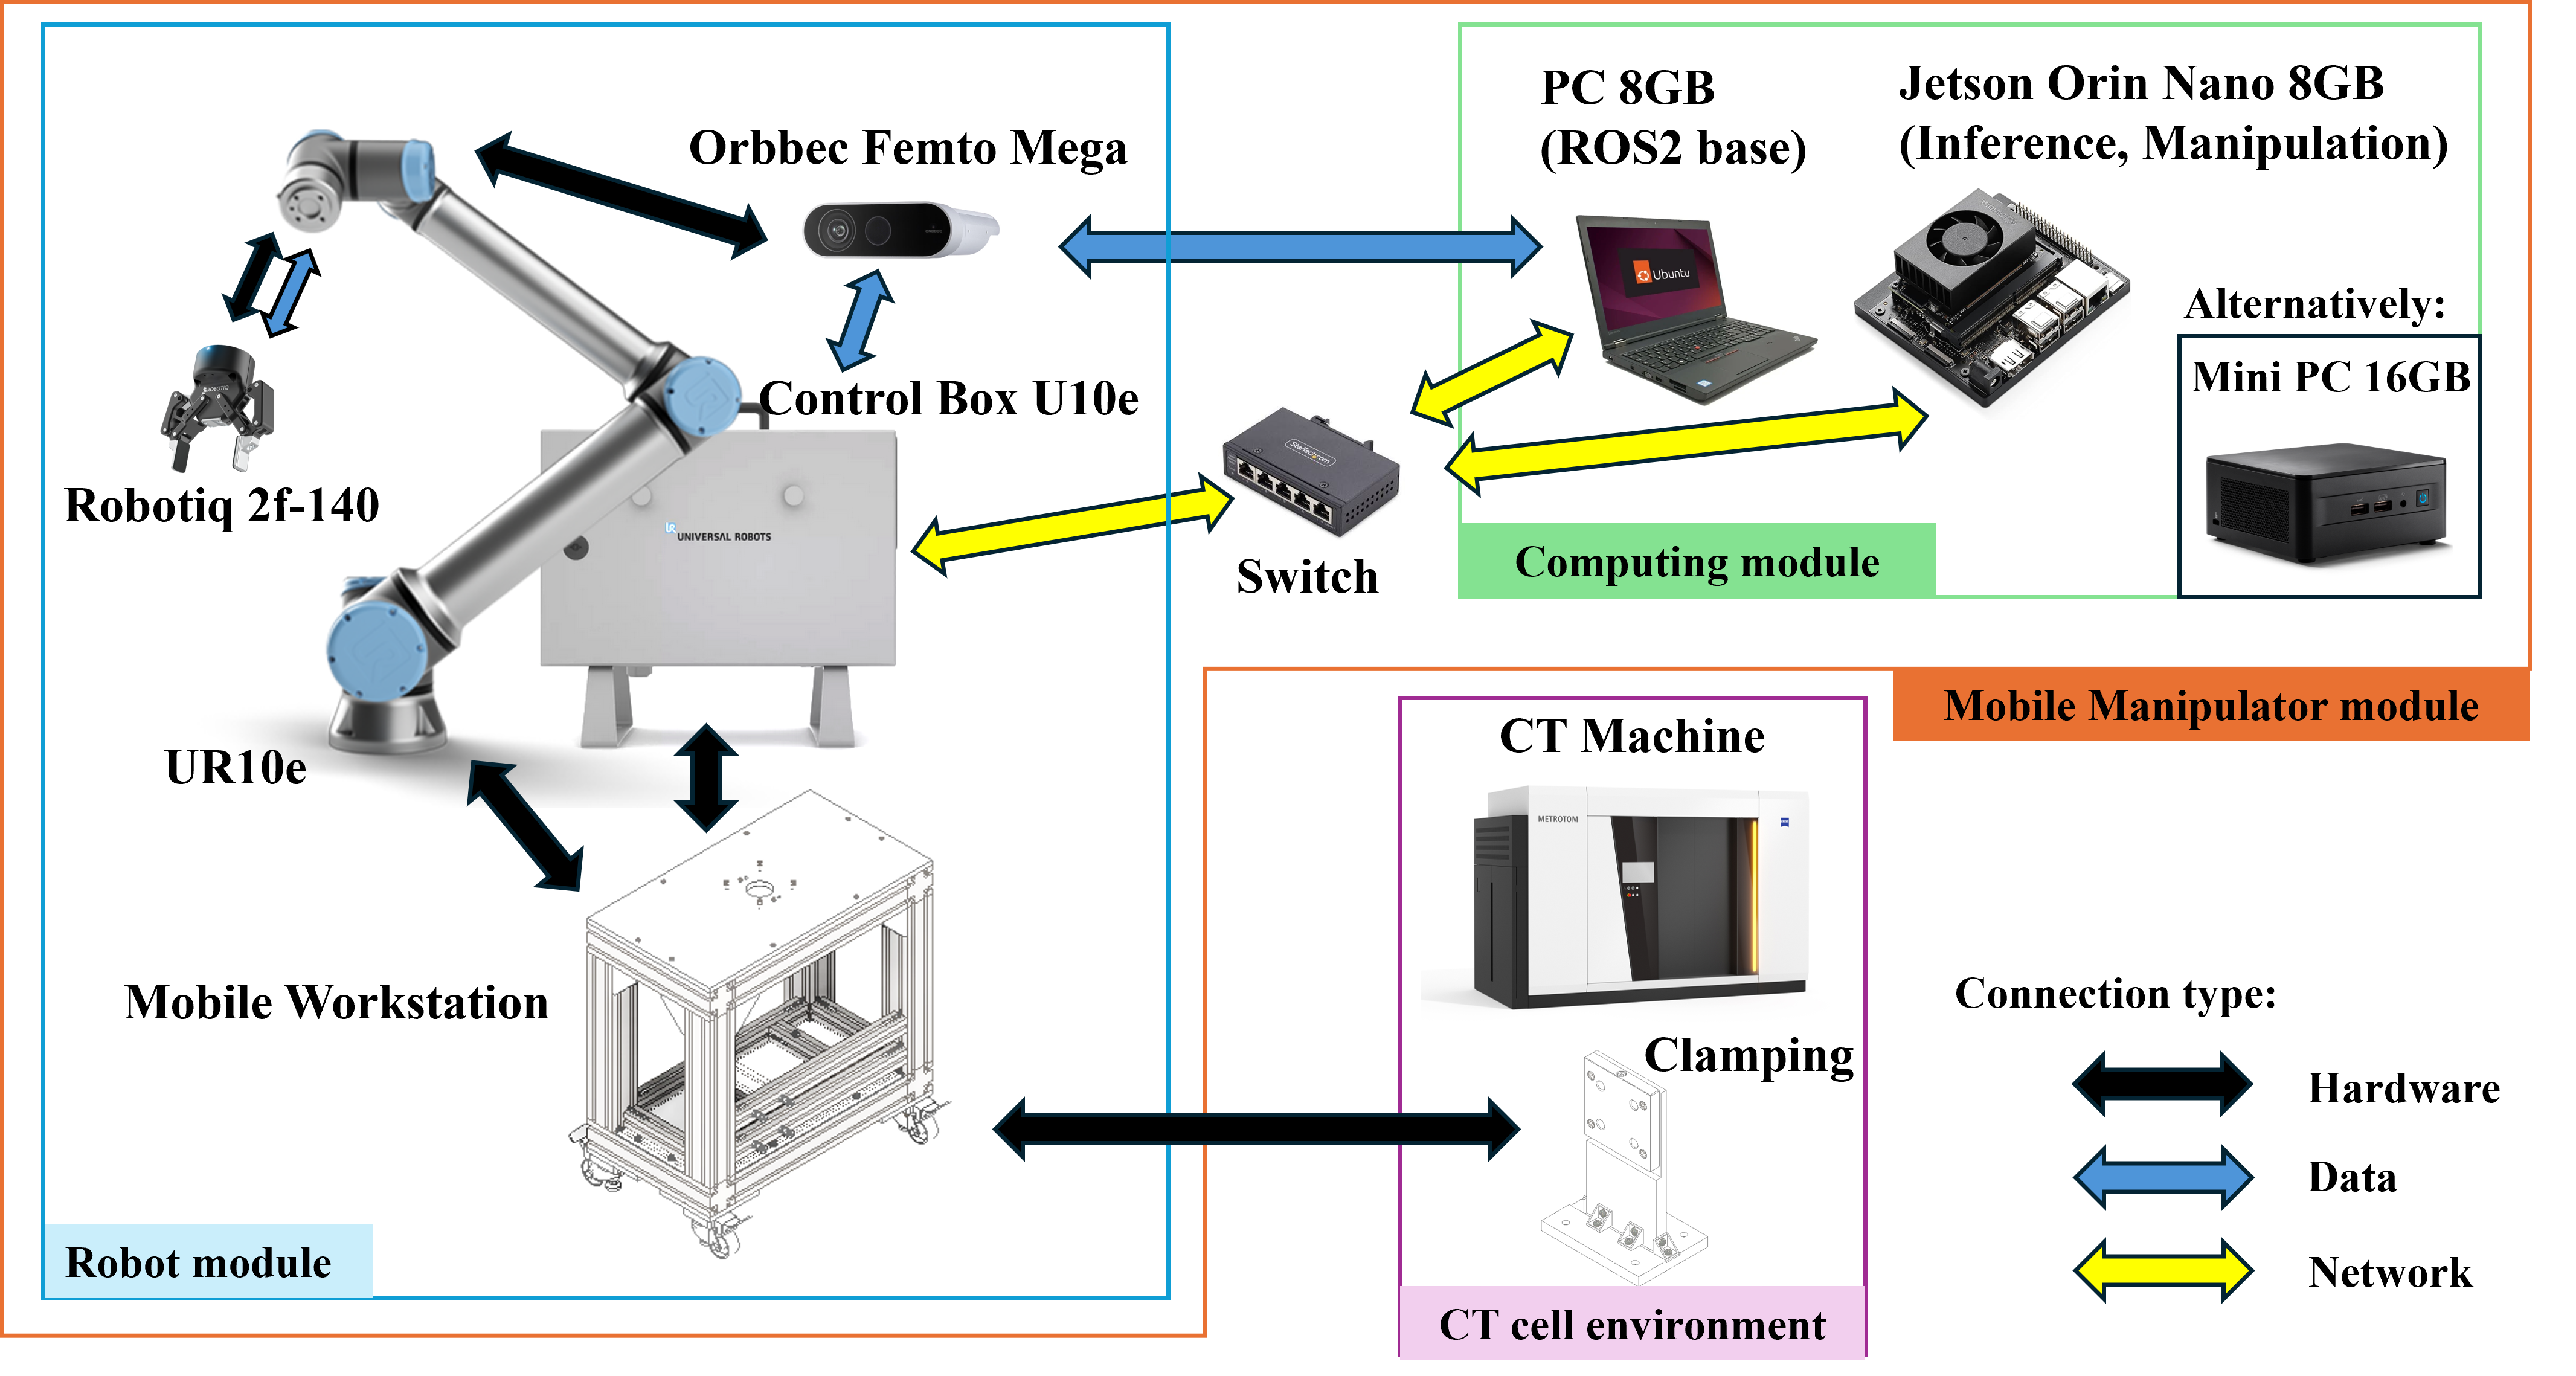
\includegraphics[width=1.0\textwidth]{hardware-config.png}
  \caption{Hardware overview. It describes the different connection types between the mobile manipulator module and the CT cell environment, as well as the internal connection between the robot module and computing module.}
  \label{fig:hardware-overview}
\end{figure}

A software stack running on the mobile manipulator module can be split into five stages and is shown in \cref{fig:software-overview}: Base (relies on ROS2), Perception (relies on Orbbec SDK), Inference (relies on vMF inference node), Planning (relies on Moveit~2) and Execution (relies on Arm API and URCaps). The used modules and nodes will be explained later in this chapter.

\begin{figure}[htbp]
  \centering
  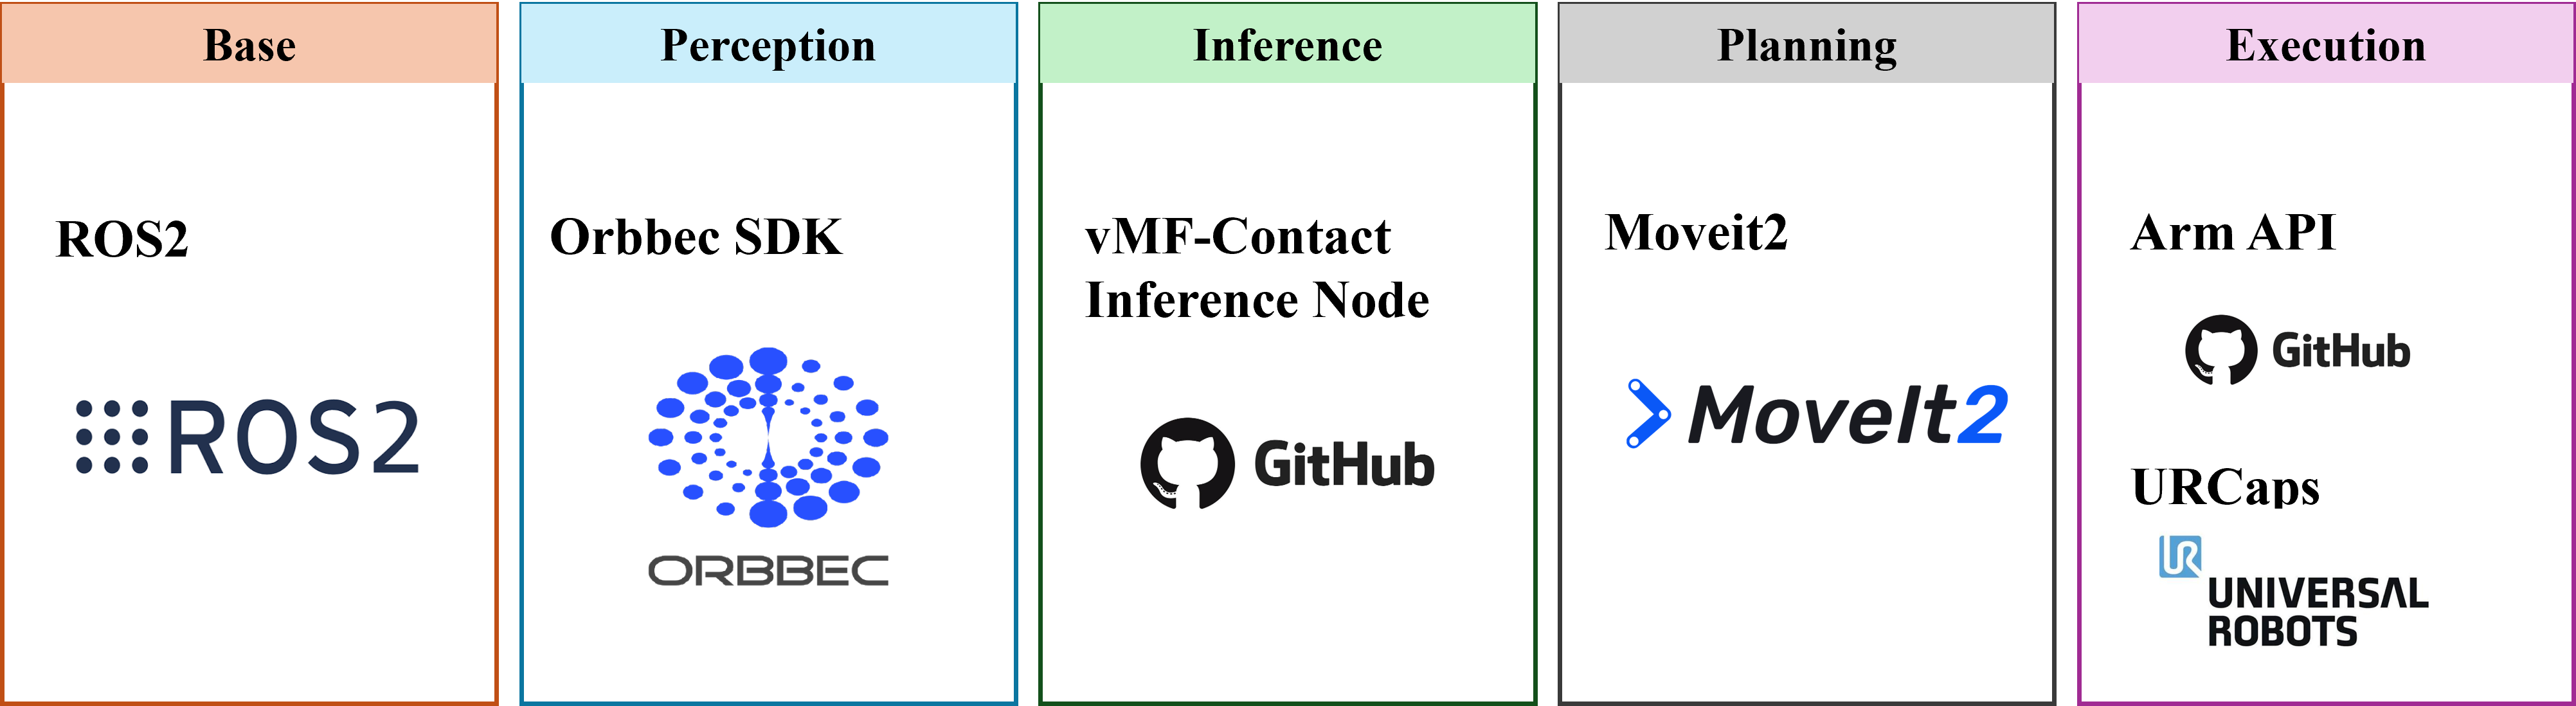
\includegraphics[width=1.0\textwidth]{software-config.png}
  \caption{Software stack overview. It describes the different modules and nodes used in all 5-stage pipeline: Base (relies on ROS2), Perception (relies on Orbbec SDK), Inference (relies on vMF inference node), Planning (relies on Moveit~2) and Execution (relies on Arm API and URCaps)}
  \label{fig:software-overview}
\end{figure}

\section{Hardware Fundamentals}
\label{sec:hardware-fundamental}

The target object evaluated throughout this thesis is an angle grinder, representative of the product class handled in the SFB-1574 cell. It has an elongated, asymmetric geometry with a cylindrical handle; its handle cross-section requires a jaw opening exceeding 85\,mm to achieve full gripper closure, which rules out the Robotiq 2F-85 and motivates the gripper selection described below.

\begin{figure}[htbp]
  \centering
  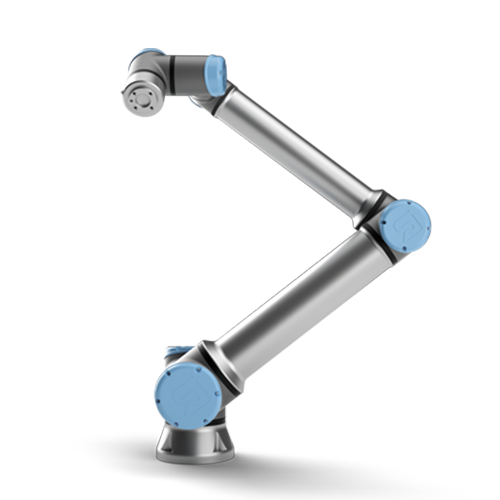
\includegraphics[width=0.5\textwidth]{ur10e.png}
  \caption{Image of Universal Robots UR10e.}
  \label{fig:ur10e}
\end{figure}

\textbf{UR10e Collaborative Robot.} The UR10e (Universal Robots, Odense, Denmark) is a 6-axis collaborative robot arm with a 1,300\,mm reach and a 12.5\,kg payload capacity. Its collaborative safety certification (ISO~10218-2) permits operation alongside an AGV delivery system without fixed physical separation. Positioning repeatability under nominal conditions is $\pm$0.05\,mm. The robot is controlled via the ROS2 Universal Robots driver, which exposes a MoveIt~2-compatible action interface for trajectory planning and execution. A product image is shown in \cref{fig:ur10e}

\begin{figure}[htbp]
  \centering
  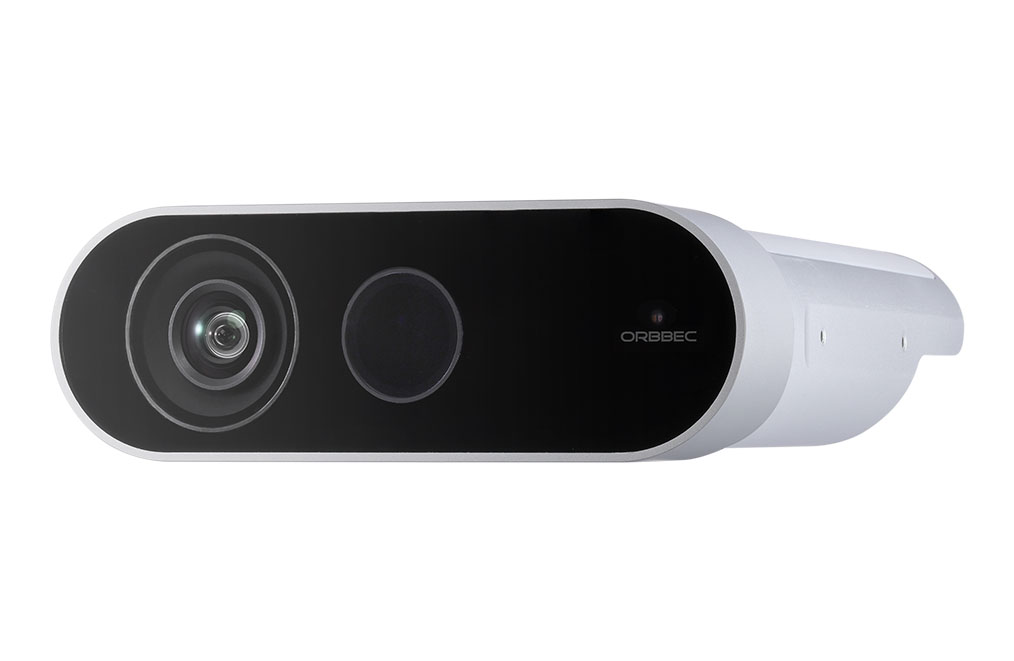
\includegraphics[width=0.3\textwidth]{orbbecfemtomega.jpg}
  \caption{Image of Orbbec Femto Mega Camera}
  \label{fig:orbbec-femto-mega}
\end{figure}

\textbf{Orbbec Femto Mega RGBD Camera.} The Orbbec Femto Mega provides structured-light depth sensing at up to 1280\,$\times$\,720 resolution over a depth range of 0.25--9.0\,m, with a nominal depth accuracy of 1--3\,mm within the operating range. The camera is mounted in a fixed eye-to-hand configuration, positioned above and lateral to the workspace to provide consistent coverage of the table surface across all object orientations. The ROS2 OrbbecSDK driver publishes registered point clouds in the camera optical frame; a calibrated static transform to the robot base frame is maintained in the TF2 tree. A product image is shown in \cref{fig:orbbec-femto-mega}

\begin{figure}[htbp]
  \centering
  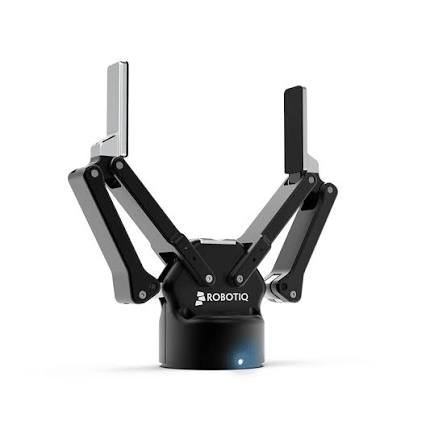
\includegraphics[width=0.3\textwidth]{robotiq.jpg}
  \caption{Image of Robotiq 2F-140 gripper.}
  \label{fig:robotiq}
\end{figure}

\textbf{Robotiq 2F-140 Gripper.} The Robotiq 2F-140 parallel-jaw gripper provides a maximum jaw opening of 140\,mm and a maximum grip force of 125\,N. The 2F-140 was selected over the Robotiq 2F-85 (85\,mm opening, 235\,N grip force) for the jaw-opening reason given above; this geometric compatibility requirement comes at the cost of lower maximum grip force, a trade-off that directly motivates the custom fingertip design described in \cref{sec:custom-fingertip-design}. The gripper communicates with the UR10e controller via Modbus TCP and is commanded from the ROS2 pipeline through a dedicated gripper driver node. A product image is shown in \cref{fig:robotiq}

\begin{figure}[htbp]
  \centering
  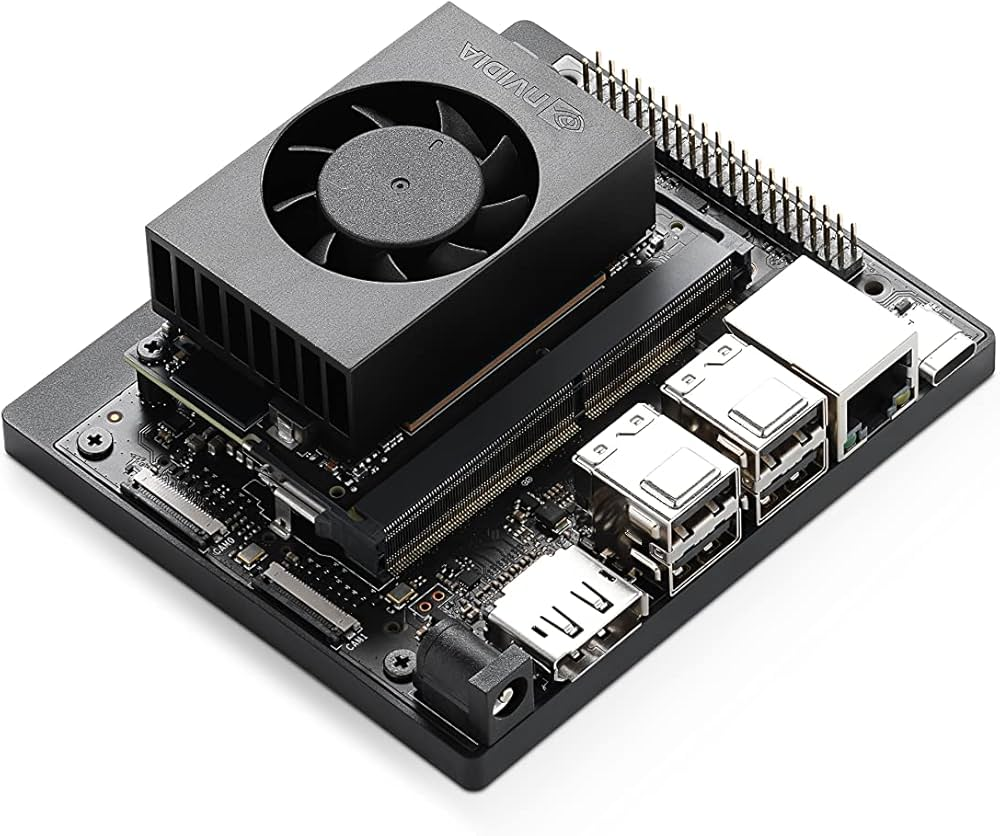
\includegraphics[width=0.4\textwidth]{jetson.jpg}
  \caption{Image of Jetson Orin Nano Super Developer Kit.}
  \label{fig:jetson}
\end{figure}

\textbf{Jetson Orin Nano Super Developer Kit.} The NVIDIA Jetson Orin Nano Super Developer Kit is a compact, high-performance edge AI platform designed for developers, researchers, and students building AI-powered applications. It delivers up to 67 INT8 TOPS of AI performance, making it suitable for demanding workloads such as computer vision, robotics, autonomous systems, and generative AI. Powered by a 6-core Arm Cortex-A78AE CPU, an NVIDIA Ampere GPU with 1,024 CUDA cores and 32 Tensor Cores, and 8 GB of LPDDR5 memory, the developer kit provides an excellent balance between performance, power efficiency and affordability. It is fully supported by the NVIDIA JetPack SDK, enabling developers to leverage CUDA, TensorRT, ROS 2, and other AI development tools for rapid prototyping and deployment of edge AI applications. A product image is shown in \cref{fig:jetson}.

\begin{figure}[htbp]
  \centering
  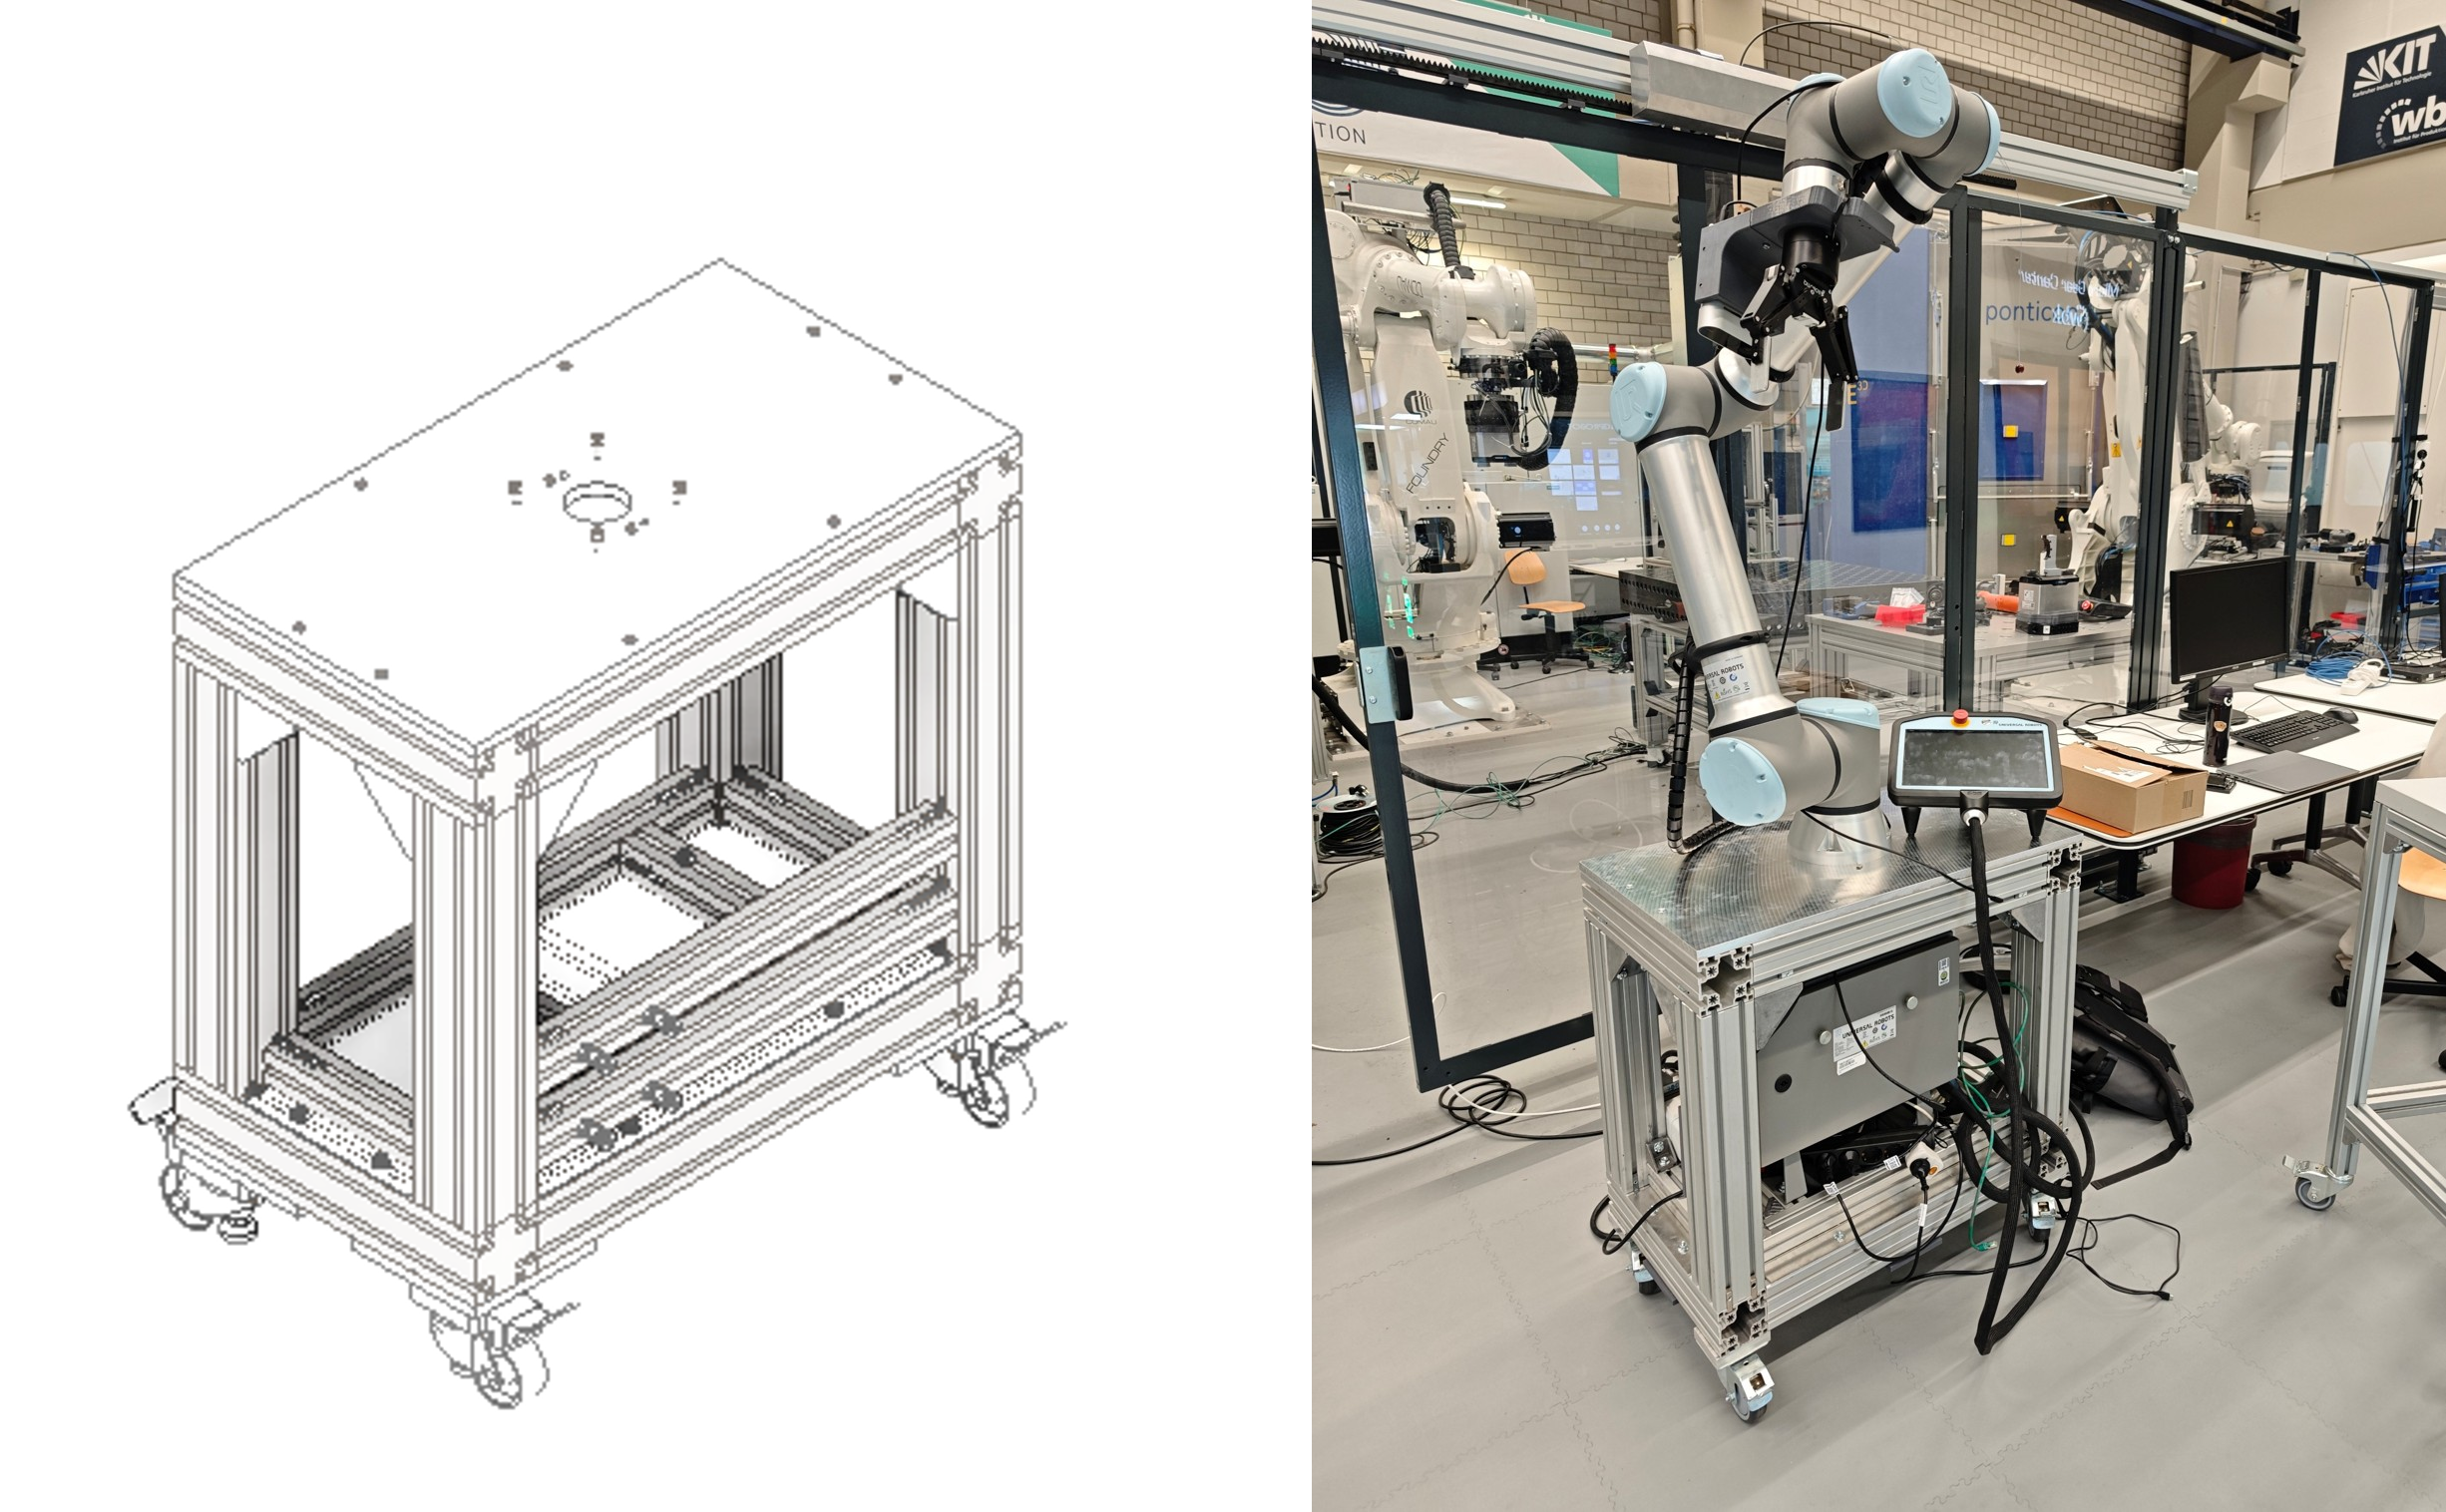
\includegraphics[width=0.5\textwidth]{robot-station-duo.png}
  \caption{Image of the robot workstation.}
  \label{fig:robot-workstation}
\end{figure}

\textbf{Robot workstation.} To enable the collaborative robot to move around in the circular factory, a workstation is designed specifically for this work. The workstation is made of Bosch Rexroth 90\,mm $\times$ 90\,mm and 45\,mm $\times$ 45\,mm aluminium profiles. It has a size of 800\,mm $\times$ 440\,mm $\times$ 850\,mm. The internal storage space can hold the control box, the network switch and other necessary IO devices. Its CAD model and actual photo is shown in \cref{fig:robot-workstation}.

\begin{figure}[htbp]
  \centering
  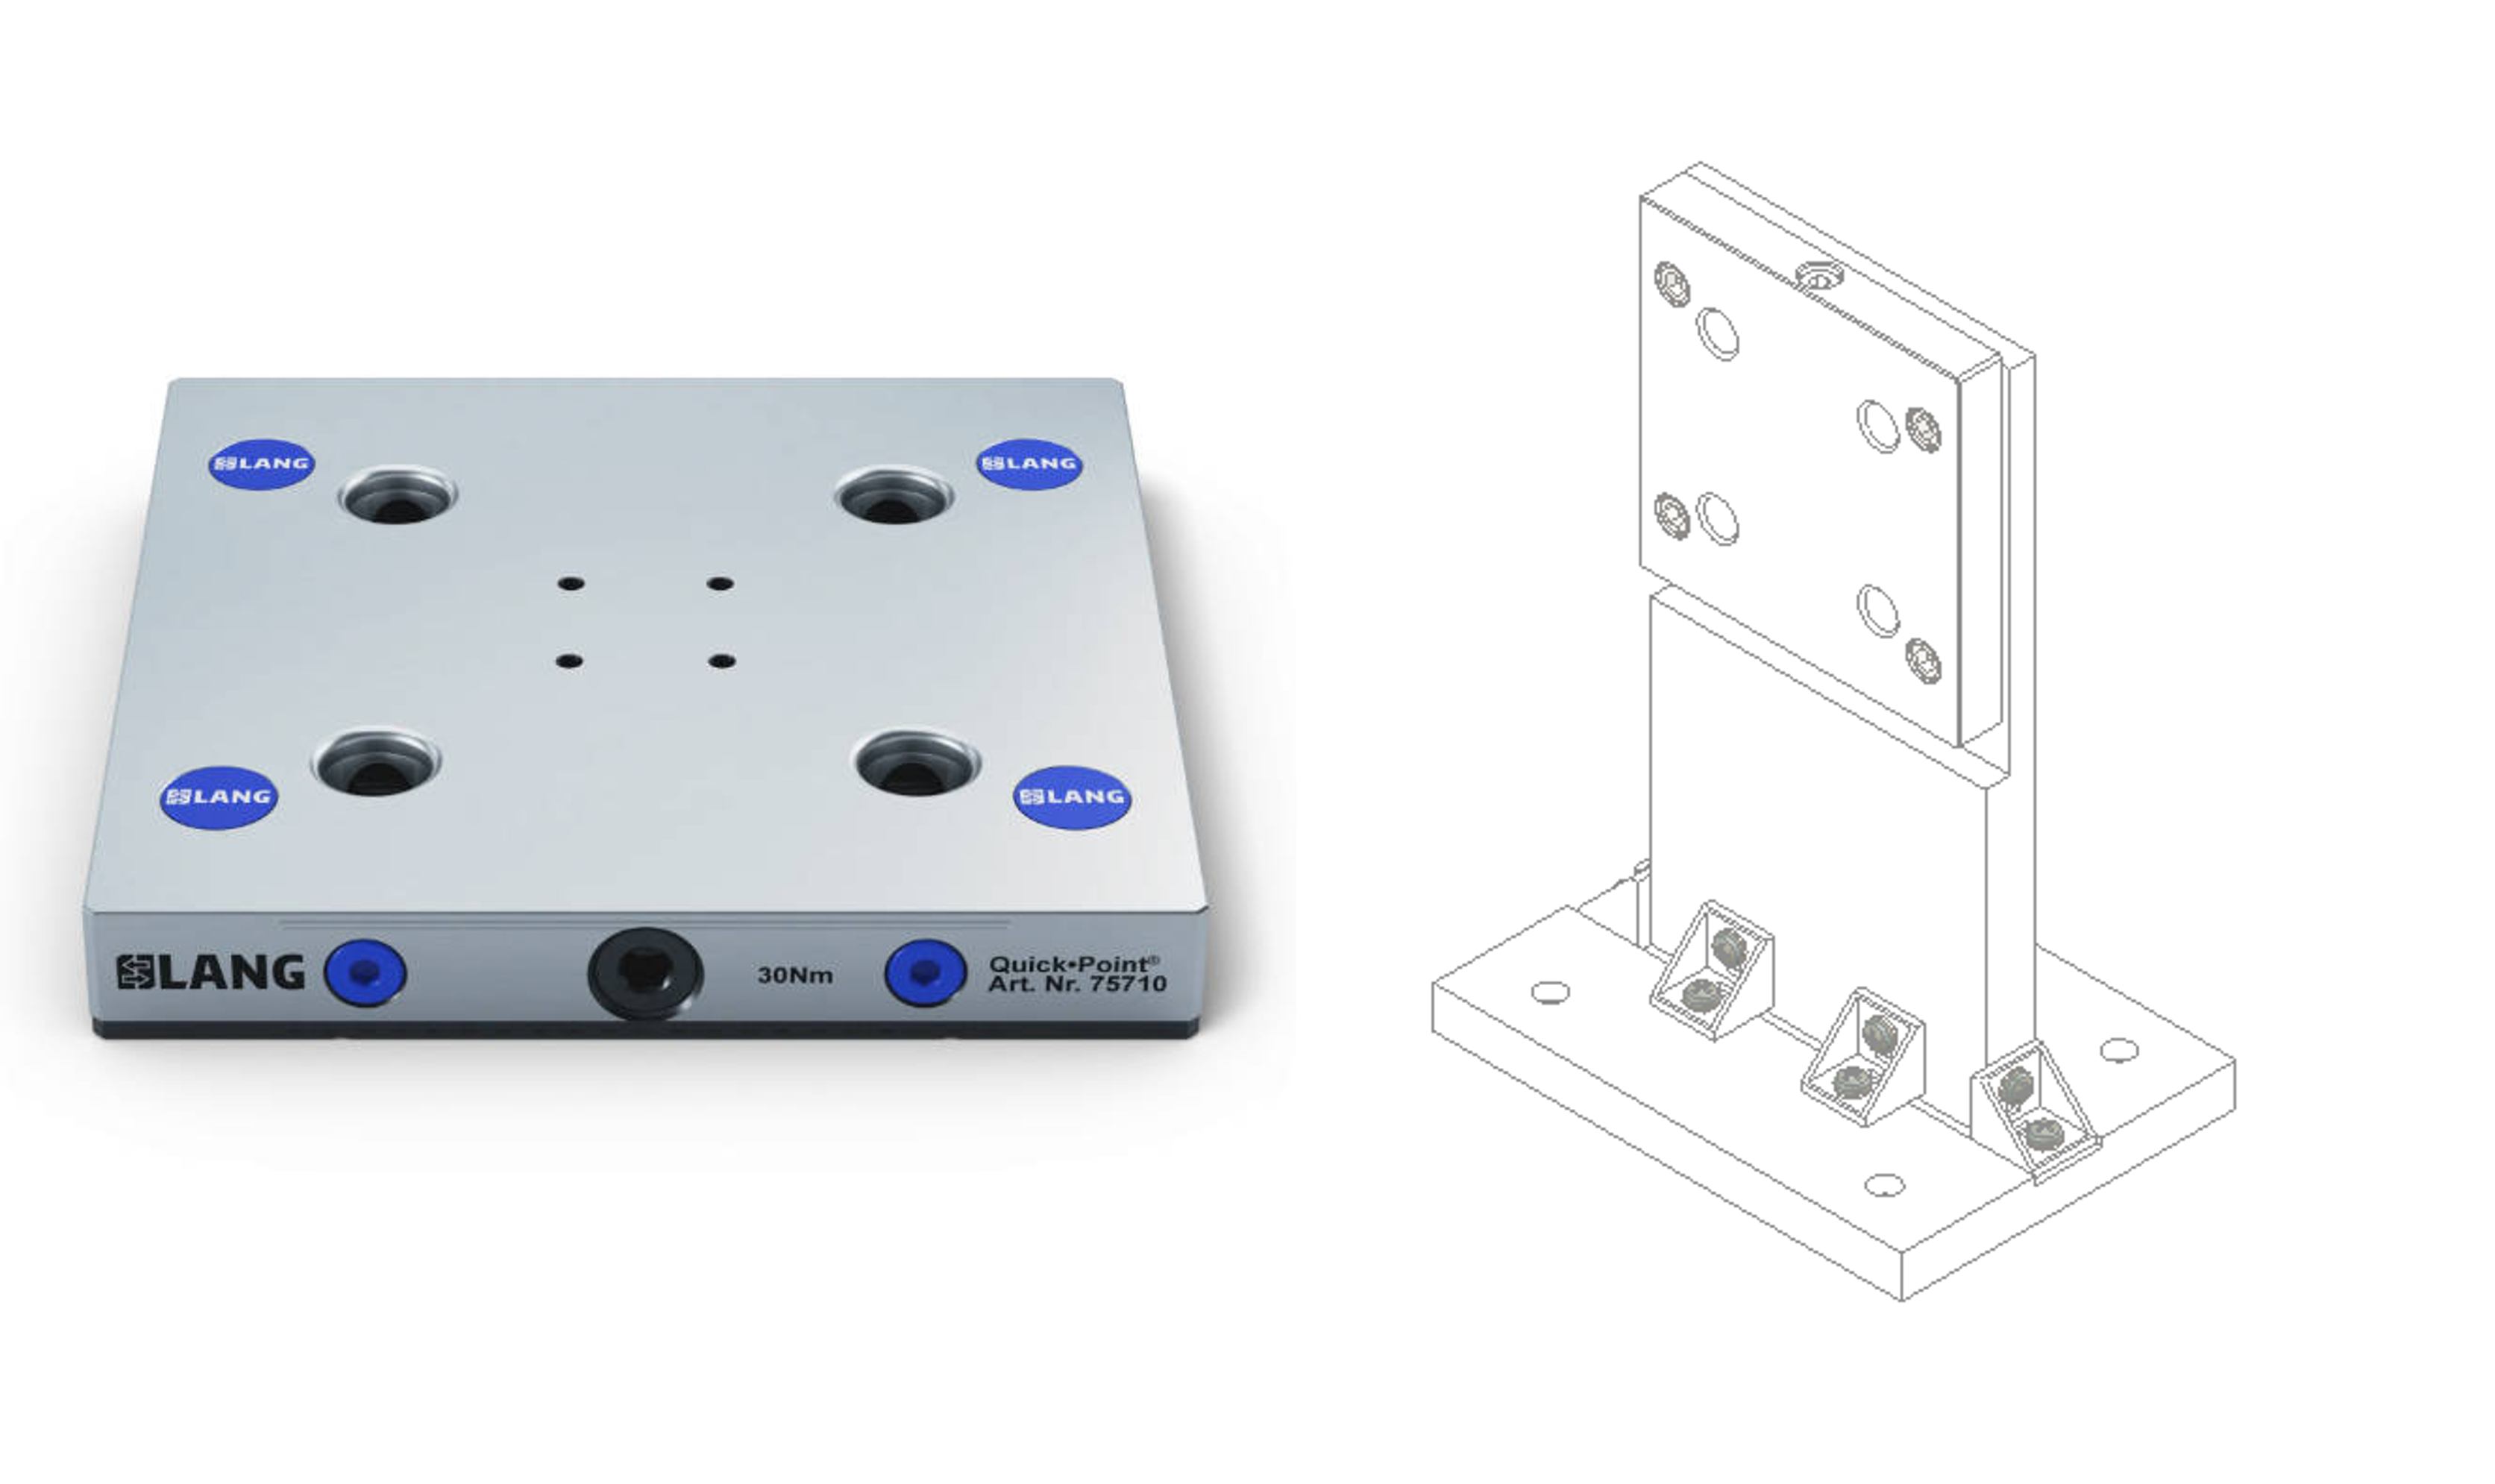
\includegraphics[width=0.5\textwidth]{clamping-duo.png}
  \caption{Image of the clamping module.}
  \label{fig:clamping}
\end{figure}

\textbf{Clamping.} To reduce the positional and orientational deviation of the mobile robot when it comes to the operating point, a clamping system which consists of a zero-point clamping module and two aluminium plates is designed. The model of the zero-point clamping module is LANG Technik Quick Point 96. It features four clamping screw holes. These holes are made to fasten the robot workstation, where 4 clamping screws are mounted on the frame of the workstation correspondingly. With this clamping mechanism, it ensures the robot always works at the same place. A product image of LANG Technik Quick Point 96 and a CAD model of the clamping system is shown in \cref{fig:clamping}. 

\section{Robot Kinematics Fundamentals}
\label{sec:robot-kinematics-fundamentals}

The UR10e is modelled as a serial kinematic chain: six revolute joints connect seven rigid links in an open chain from the base to the end-effector flange. Each link's pose relative to its neighbour is a rigid-body transformation in $SE(3)$, combining a rotation and a translation and represented as a $4\times4$ homogeneous transformation matrix. The Denavit--Hartenberg (DH) convention~\cite{denavit1955kinematic} parameterises each joint-to-joint transform with four quantities --- link length $a_i$, link twist $\alpha_i$, link offset $d_i$, and joint angle $\theta_i$ --- combined into a single homogeneous transform~\cite{siciliano2009robotics}:

\begin{equation}\label{eq:dh-transform}
  A_i(\theta_i) =
  \begin{bmatrix}
    \cos\theta_i & -\sin\theta_i\cos\alpha_i & \sin\theta_i\sin\alpha_i & a_i\cos\theta_i \\
    \sin\theta_i & \cos\theta_i\cos\alpha_i & -\cos\theta_i\sin\alpha_i & a_i\sin\theta_i \\
    0 & \sin\alpha_i & \cos\alpha_i & d_i \\
    0 & 0 & 0 & 1
  \end{bmatrix}
\end{equation}

The four parameters follow from a frame assignment rule applied at every joint: the $z_{i-1}$ axis is aligned with joint $i$'s axis of rotation, and the $x_i$ axis is aligned with the common normal between $z_{i-1}$ and $z_i$ --- the unique line perpendicular to both consecutive joint axes. This choice of frame gives each of the four DH parameters a direct geometric reading:

\begin{itemize}
  \item $a_i$ (link length) --- the distance between the $z_{i-1}$ and $z_i$ axes, measured along their common normal. It is fixed by the physical offset between two consecutive joints and is zero when consecutive joint axes intersect.
  \item $\alpha_i$ (link twist) --- the angle between the $z_{i-1}$ and $z_i$ axes, measured about the common normal. It is zero when consecutive joint axes are parallel, as is the case for several joint pairs in the UR10e's shoulder and elbow.
  \item $d_i$ (link offset) --- the distance along $z_{i-1}$ from frame $i-1$'s origin to the point where the common normal crosses $z_{i-1}$. For a prismatic joint this quantity is the joint variable; for the UR10e's revolute joints it is a fixed geometric constant.
  \item $\theta_i$ (joint angle) --- the angle about $z_{i-1}$ from the $x_{i-1}$ axis to the $x_i$ axis. For a revolute joint this is the joint variable read directly from the arm's encoders.
\end{itemize}

\begin{figure}[htbp]
  \centering
  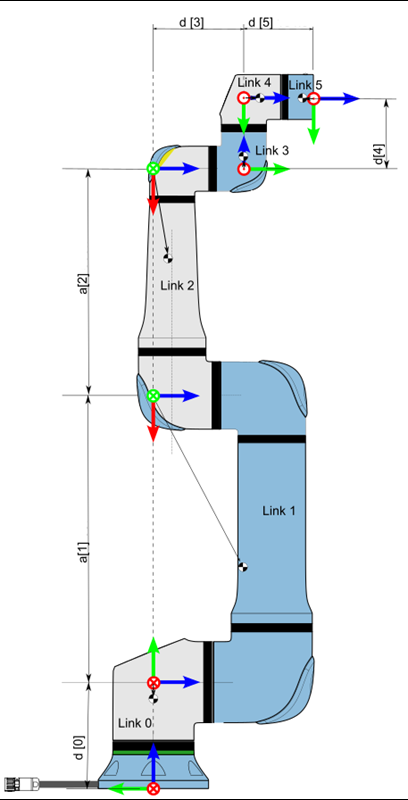
\includegraphics[width=0.6\textwidth]{ur-kinematcis.png}
  \caption{The Denavit-Hartenberg parameters of a UR robot. Adapted from~\cite{universalrobots2024dh}}
  \label{fig:ur-dh}
\end{figure}

\cref{fig:ur-dh} shows the Denavit-Hartenberg parameters of a 6-axis UR robot. Consequently, for the UR10e's all-revolute structure, $\theta_i$ is the only quantity that changes as the arm moves; $a_i$, $\alpha_i$, and $d_i$ are constants fixed by the manufacturer's link dimensions and are tabulated once per robot model. This factorisation is what makes a 6-axis arm tractable to reason about: each joint contributes one matrix of the form in \cref{eq:dh-transform}, built from one variable and three constants, and the chain composes these matrices in sequence from base to flange.

\cref{tab:ur10e-dh-parameters} lists the manufacturer-published values of $a_i$, $d_i$, and $\alpha_i$ for the UR10e~\cite{universalrobots2024dh}; the same parameter set is shared with the UR12e. The joint angles $\theta_i$ are omitted from the table because they are not fixed geometric constants: they are the joint variables read from the arm's encoders at run time.

\begin{table}[htbp]
  \centering
  \caption{Denavit--Hartenberg kinematic parameters for the UR10e, as published by the manufacturer~\cite{universalrobots2024dh}.}
  \label{tab:ur10e-dh-parameters}
  \begin{tabular}{crrr}
    \toprule
    Joint $i$ & $a_i$ [m] & $d_i$ [m] & $\alpha_i$ [rad] \\
    \midrule
    1 & 0        & 0.1807  & $\pi/2$  \\
    2 & -0.6127  & 0       & 0        \\
    3 & -0.57155 & 0       & 0        \\
    4 & 0        & 0.17415 & $\pi/2$  \\
    5 & 0        & 0.11985 & $-\pi/2$ \\
    6 & 0        & 0.11655 & 0        \\
    \bottomrule
  \end{tabular}
\end{table}

% TODO: insert figure of the UR10e frame assignment / DH parameter diagram here.

Substituting a table row's $a_i$, $d_i$, $\alpha_i$ together with the corresponding run-time $\theta_i$ into \cref{eq:dh-transform}, then chaining the six resulting matrices per \cref{eq:fk-chain}, gives the UR10e's forward kinematics in closed form.

\textbf{Forward kinematics.} Given the six joint angles $(\theta_1, \dots, \theta_6)$, forward kinematics computes the end-effector pose $T_6^0$ relative to the base frame as the product of the six per-joint DH transforms along the chain:

\begin{equation}\label{eq:fk-chain}
  T_6^0(\theta_1, \dots, \theta_6) = A_1(\theta_1)\,A_2(\theta_2)\,A_3(\theta_3)\,A_4(\theta_4)\,A_5(\theta_5)\,A_6(\theta_6)
\end{equation}

This mapping from joint space to task space is unique and always defined: every joint configuration produces exactly one end-effector pose via \cref{eq:fk-chain}, and evaluating it involves no search or iteration.

\textbf{Inverse kinematics.} The inverse problem, central to grasp execution, asks the opposite question: given a target end-effector pose, such as a grasp candidate surviving the constraint filters in \cref{sec:vmf-contact-inference}, which joint configuration reaches it, i.e.\ which $\theta = (\theta_1, \dots, \theta_6)$ satisfies $T_6^0(\theta) = T_{\mathrm{target}}$. Inverse kinematics (IK) lacks the forward problem's uniqueness. A 6-DoF non-redundant arm can admit several joint solutions for the same reachable pose (e.g.\ elbow-up and elbow-down configurations); some poses admit no solution because they lie outside the arm's reachable workspace or would require exceeding a joint limit; and the mapping becomes locally non-invertible at kinematic singularities.

Singularities and the local relationship between joint motion and end-effector motion are captured by the manipulator Jacobian $J(\theta) \in \mathbb{R}^{6\times6}$, which relates joint velocities $\dot{\theta}$ to end-effector linear velocity $v$ and angular velocity $\omega$:

\begin{equation}\label{eq:jacobian-velocity}
  \begin{bmatrix} v \\ \omega \end{bmatrix} = J(\theta)\,\dot{\theta}
\end{equation}

For an arm built entirely of revolute joints, the $i$-th column of $J(\theta)$ is

\begin{equation}\label{eq:jacobian-column}
  J_i(\theta) =
  \begin{bmatrix}
    z_{i-1} \times (o_6 - o_{i-1}) \\
    z_{i-1}
  \end{bmatrix}
\end{equation}

where $z_{i-1}$ is the axis of joint $i$ and $o_{i-1}$, $o_6$ are the origins of joint $i$ and the end-effector frame, respectively, all expressed in the base frame and obtained from the intermediate transforms in \cref{eq:fk-chain}. A configuration is singular when $\det J(\theta) = 0$, i.e.\ when $J(\theta)$ drops below full rank; at such configurations, \cref{eq:jacobian-velocity} cannot be inverted, and small task-space motions would require unboundedly large joint velocities.

Closed-form analytical solutions of $T_6^0(\theta) = T_{\mathrm{target}}$ exist for the six-revolute-joint structure common to industrial arms including the UR10e~\cite{siciliano2009robotics}; where collision geometry or joint-limit padding must additionally be respected, the motion planner instead solves IK numerically, iterating an update of the form

\begin{equation}\label{eq:jacobian-ik-update}
  \theta_{k+1} = \theta_k + J(\theta_k)^{+}\left(x_{\mathrm{target}} - f(\theta_k)\right)
\end{equation}

where $f(\theta_k)$ is the end-effector pose at the current iterate (\cref{eq:fk-chain}), $x_{\mathrm{target}}$ is the target pose, and $J(\theta_k)^{+}$ is the Jacobian pseudoinverse, until the iterate converges to a feasible joint configuration or the search is exhausted.

Reachable workspace, joint limits, and singularities are the three constraints that determine whether an otherwise valid grasp candidate is executable. \cref{sec:software-fundamentals} describes how MoveIt~2 embeds this IK step inside its collision-aware trajectory planning; failures of this planning step against these same three constraints are the kinematic infeasibility failure mode reported in \cref{sec:failure-mode-definitions}.

\section{Software Fundamentals}
\label{sec:software-fundamentals}

\textbf{ROS2.} The Robot Operating System~2 (ROS2) is the middleware framework underlying the software stack. It organises the system as a graph of independent nodes exchanging messages over topics, services, and actions, built on the Data Distribution Service (DDS) standard for inter-process communication. This thesis uses the Humble Hawksbill long-term support release running on Ubuntu 22.04. Nodes for perception, inference, motion planning, and robot control communicate through this framework; the specific containerised arrangement of these nodes is described in \cref{sec:docker-configuration}.

\textbf{Orbbec~SDK.} The Orbbec~SDK is a cross-platform software development kit for Orbbec 3~D depth cameras, providing a unified interface to access RGB, depth, IMU, and point cloud data. It enables developers to configure camera parameters, synchronize sensors, process depth images, and generate 3~D point clouds. With its high-level APIs, sample applications, and support for robotics frameworks such as ROS~2, the Orbbec~SDK simplifies the development of computer vision, robotics, and 3~D perception applications.

\textbf{vMF-Contact Inference Node.} The vMF-Contact inference node is the core of the manipulating process. It generates grasp candidates based on von Mises-Fisher distribution and assigns grasp confidence to every grasp candidate. It will be introduced in \cref{sec:uncertainty-aware-grasping} in detail.

\begin{figure}[htbp]
  \centering
  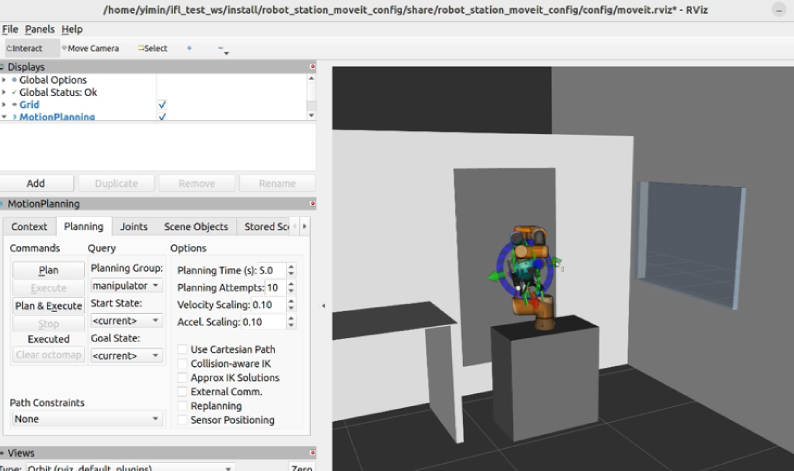
\includegraphics[width=0.6\textwidth]{moveit-screenshot.jpg}
  \caption{Screenshot of MoveIt~2.}
  \label{fig:moveit-screenshot}
\end{figure}

\textbf{MoveIt~2.} MoveIt~2 is the ROS~2 motion planning framework used to compute collision-aware joint trajectories for the UR10e. Given a target end-effector pose, MoveIt~2 samples and optimises a trajectory through the robot's configuration space that respects joint limits, self-collision constraints, and the collision geometry of the environment, using the UR10e's Unified Robot Description Format (URDF) model. The planned trajectory is then handed to the robot controller for execution. A screenshot of MoveIt~2 is shown in \cref{fig:moveit-screenshot}.

\textbf{Arm API~2.} Arm API2 is intended to provide interfacing support for robot manipulators for ROS~2 and MoveIt~2, enabling users to use one interface for multiple arms (Franka, Kinova, UR) and switch between planning and servo workflows without changing the app structure. With the ArmApi2Client class, user can control a robotic arm using ROS 2 actions and services. This client allows user to set velocity and acceleration scaling factors, change the arm's state, control the gripper, and move the arm to specified poses or joint positions.

\textbf{Cartesian Pose Interpolation.} For point-to-point Cartesian moves, the \texttt{ArmApi2Client} produces the intermediate trajectory itself, rather than routing every waypoint through MoveIt~2's joint-space planner. Each commanded move proceeds through the same six steps:

\begin{enumerate}
  \item \textbf{Read the start pose.} The current end-effector pose is read from the robot state. If the current pose and the target pose are not already expressed in the same frame, both are transformed into the MoveIt planning frame.
  \item \textbf{Check whether the move is reasonable.} The straight-line distance between the current and target positions and the rotation difference between the current and target orientations are computed. If either exceeds a configured threshold, the move is treated as too large for direct interpolation and the step is skipped.
  \item \textbf{Build a motion profile.} From the configured average velocity and acceleration, a time profile for the move is estimated: constant-speed for very short moves, triangular (accelerate then decelerate, no cruise phase) for moves too short to reach the target speed, or trapezoidal (accelerate, cruise, decelerate) otherwise.
  \item \textbf{Generate intermediate poses.} The motion profile is sampled at several time points between start and target. At each sample, the position is interpolated linearly between the start and target positions, and the orientation is interpolated with spherical linear interpolation (SLERP)~\cite{shoemake1985animating}, which follows the shortest arc between the two orientations on the unit-quaternion sphere rather than a linear blend of Euler angles.
  \item \textbf{Send the poses.} Each interpolated pose is published in sequence as a pose command, with a sleep interval between successive commands matched to the sampling interval of the motion profile, so the end-effector traces the interpolated path at the intended speed instead of jumping between waypoints.
  \item \textbf{Remember the end pose.} After the last sample is published, the final interpolated pose is stored as the client's current pose, so that the next commanded move starts its distance and profile calculations from this pose rather than re-reading a possibly stale robot state.
\end{enumerate}

In effect, this turns one large Cartesian move into a series of short, smoothly changing pose commands, so the end-effector appears to move continuously from the current pose to the target pose rather than snapping directly to it. The interpolator is a Cartesian-space complement to MoveIt~2's joint-space planning above: it is not collision-aware, and the distance and orientation check in step~2 is its only safeguard against an unreasonably large or discontinuous move; such moves are instead left to MoveIt~2's planner.

\textbf{URCaps and External Control.} The UR10e control box runs Universal Robots' proprietary control software, which is extended through URCaps, a plugin interface for installing additional applications on the robot controller. The ROS2 Universal Robots driver requires the External Control URCap to be installed and active on the controller: it hands trajectory execution authority from the robot's native teach-pendant programs to an external ROS2 client. In this work URCaps and external control is mainly used with Arm API~2.

% ============================================================
\chapter{Related Work}
\label{chap:related-work}
% ============================================================

\section{Model-Based Grasping}
\label{sec:model-based-grasping}

Robotic grasping relies on contact mechanics and force-closure analysis. \cite{bicchi2000robotic} built the analytical framework for grasp stability. It models contact forces, friction, and force-closure kinematics. These principles still underlie model-based grasp evaluation today. They also indirectly shape learning-based grasp evaluation methods. 

Model-based systems pair pose estimation with a pre-programmed grasp. They start with a CAD model and a depth-sensor point cloud. ICP~\cite{besl1992} aligns the scan to the stored model. This recovers the object's pose. A robot program then executes the matching grasp. \cite{rusu2009fast} added Fast Point Feature Histograms (FPFH) to the toolkit. FPFH encodes local surface curvature into compact feature vectors. This enables faster convergence than nearest-point search alone. It also improves ICP initialisation under partial occlusion. The Point Cloud Library (PCL)~\cite{rusu2011pcl} consolidated these point-cloud algorithms. PCL became a widely used open-source framework. It underpins most depth-sensor-based robotic perception pipelines.

Simulation tools like GraspIt!~\cite{miller2004graspit} enabled analytical grasp evaluation. They let researchers enumerate and score grasps before deployment. This accelerated model-based grasp system development. It also generated grasp databases for later data-driven methods. \cite{bohg2014data} surveyed data-driven grasp synthesis across both paradigms. They mapped object representations, grasp types, and end-effector morphology. Their survey names known geometry as the key limitation. This motivates the learning-based methods in \cref{sec:learning-based-grasping}.

Model-based grasping assumptions restrict its operating envelope. ICP needs the scanned object to match the model closely. Surface wear or deformation can break this match. A fixed line with one product variant meets this need. A return stream with varied products usually does not. No parameter tuning can fix this fundamental limitation. ICP always assumes a known, stable geometry. This motivates the shift to learning-based approaches.

\section{Learning-Based Grasping}
\label{sec:learning-based-grasping}

\subsection{2D Grasp Detection: Foundational Approaches}
\label{sec:2d-grasp-detection}

Early learning-based grasping treated the task as 2D prediction. \cite{jiang2011efficient} introduced a rectangle representation for two-finger grasps. It used RGBD data without needing a CAD model. This enabled efficient search over candidate grasp configurations. \cite{lenz2015deep} trained a two-stage network on labelled RGBD patches. It reliably scored grasp quality on novel household objects. This showed deep learning could replace hand-crafted grasp features. \cite{redmon2015realtime} ran single-pass convolutional networks at interactive frame rates. This enabled real-time, reactive grasp detection. \cite{kumra2017robotic} fine-tuned ImageNet-pretrained residual networks for grasp detection. Accuracy stayed strong despite this cross-domain transfer. This confirmed image-classification transfer learning helps grasp detection.

These 2D approaches share one key limitation. They output only planar position, orientation, and opening width. They cannot directly generate full 6-DoF grasp poses. So their use is limited to controlled table-top settings. The object must lie flat in these settings. The camera-to-robot transformation must also stay fixed.

\subsection{6-DoF Grasp Generation from Point Clouds}
\label{sec:6dof-grasping}

6-DoF grasp generation emerged to handle arbitrary orientations and clutter. Grasp Pose Detection (GPD)~\cite{tenPas2017} scored 6-DoF grasps from point-cloud patches. It needed no per-object programming to work. GPD learned geometric features tied to stable contact. It generalised to novel object geometries at test time. This showed grasp quality is a learnable geometric function.

Point-cloud architecture advances became the backbone for grasp networks. PointNet~\cite{qi2017pointnet} was the first network on raw point sets. It preserved sensor fidelity without voxelisation or projection loss. Symmetric aggregation gave it permutation-invariant, preprocessing-free design. PointNet++~\cite{qi2017pointnet2} added hierarchical, multi-scale set abstraction layers. \cite{wang2019dgcnn} introduced Dynamic Graph CNN (DGCNN) for point clouds. DGCNN builds a dynamic nearest-neighbour graph in feature space. Edge convolutions then capture higher-order surface relationships. \cite{zhao2021point} added self-attention with Point Transformer for point sets. Attention-weighted aggregation gave strong local feature discrimination. These architectures became standard grasp-network backbones. They enabled richer surface representations than 2D approaches.

Data collection and analytic metrics also drove progress. \cite{levine2018learning} learned hand-eye coordination from millions of real attempts. No explicit geometric model was needed for this. It improved continuously from grasp outcome feedback. \cite{mahler2017dexnet} (Dex-Net 2.0) combined simulated analytic metrics with deep learning. It trained on synthetic point clouds for robustness guarantees. \cite{mousavian2019grasp} (6-DOF GraspNet) generated diverse 6-DoF grasps variationally. This explored many candidates instead of a fixed set. \cite{morrison2020learning} (GG-CNN) traded accuracy for 50\,Hz reactive grasping speed. \cite{mahler2018dexnet3} extended Dex-Net to vacuum suction grasping (Dex-Net 3.0). This showed analytic-plus-learning hybrids transfer across end-effector types.

GraspNet-1Billion~\cite{fang2020} built a large systematic grasping benchmark. It has one billion annotated 6-DoF poses across 88 categories. A subset also received real-world evaluation. The dataset proved methods can transfer across object classes. This was a qualitative advance over per-object programming. It also standardised the protocol for comparing methods. Success rates above 70\,\% became the field's reference point.

Contact-GraspNet~\cite{sundermeyer2021} advanced grasping in cluttered scenes. It samples candidates directly from predicted surface contact points. This works well even under partial occlusion. \cite{breyer2021volumetric} used a volumetric network at interactive frame rates. It kept candidate quality while cutting inference latency. These systems mark the current ceiling for deterministic methods.

\cite{kroemer2021review} reviewed architectures, data needs, and task formulations broadly. They name one central unresolved challenge for real-world manipulation. It is the gap between benchmarks and unstructured deployment.

These benchmarks all assume controlled, consistent evaluation conditions. Lighting, placement, and object sets stay fixed and known. None of these works address the real-deployment gap. That gap simply falls outside their intended scope. Still, this gap matters a great deal. A 70\,\% laboratory success rate predicts nothing about deployment.

\section{Uncertainty-Aware Grasping and vMF-Contact}
\label{sec:uncertainty-aware-grasping}

Deterministic networks give each candidate one quality score. They encode no confidence about that prediction. For well-represented objects, this score reliably tracks grasp stability. For novel or occluded geometries, that correlation weakens. Yet the network still reports equally confident-looking scores. It gives no signal that the prediction is unreliable. A deterministic ranker cannot tell confidence from a guess.

\cite{gal2016dropout} formalised statistical uncertainty in neural network predictions. Monte Carlo dropout approximates Bayesian inference tractably. It estimates epistemic uncertainty without changing the training objective. \cite{kendall2017uncertainties} then split uncertainty into two distinct sources. Aleatoric uncertainty comes from observation noise and is irreducible. Epistemic uncertainty comes from limited data coverage and is reducible. \cite{lakshminarayanan2017simple} showed network ensembles give well-calibrated uncertainty estimates. This simple method became a common Bayesian-method baseline.

\begin{figure}[htbp]
  \centering
  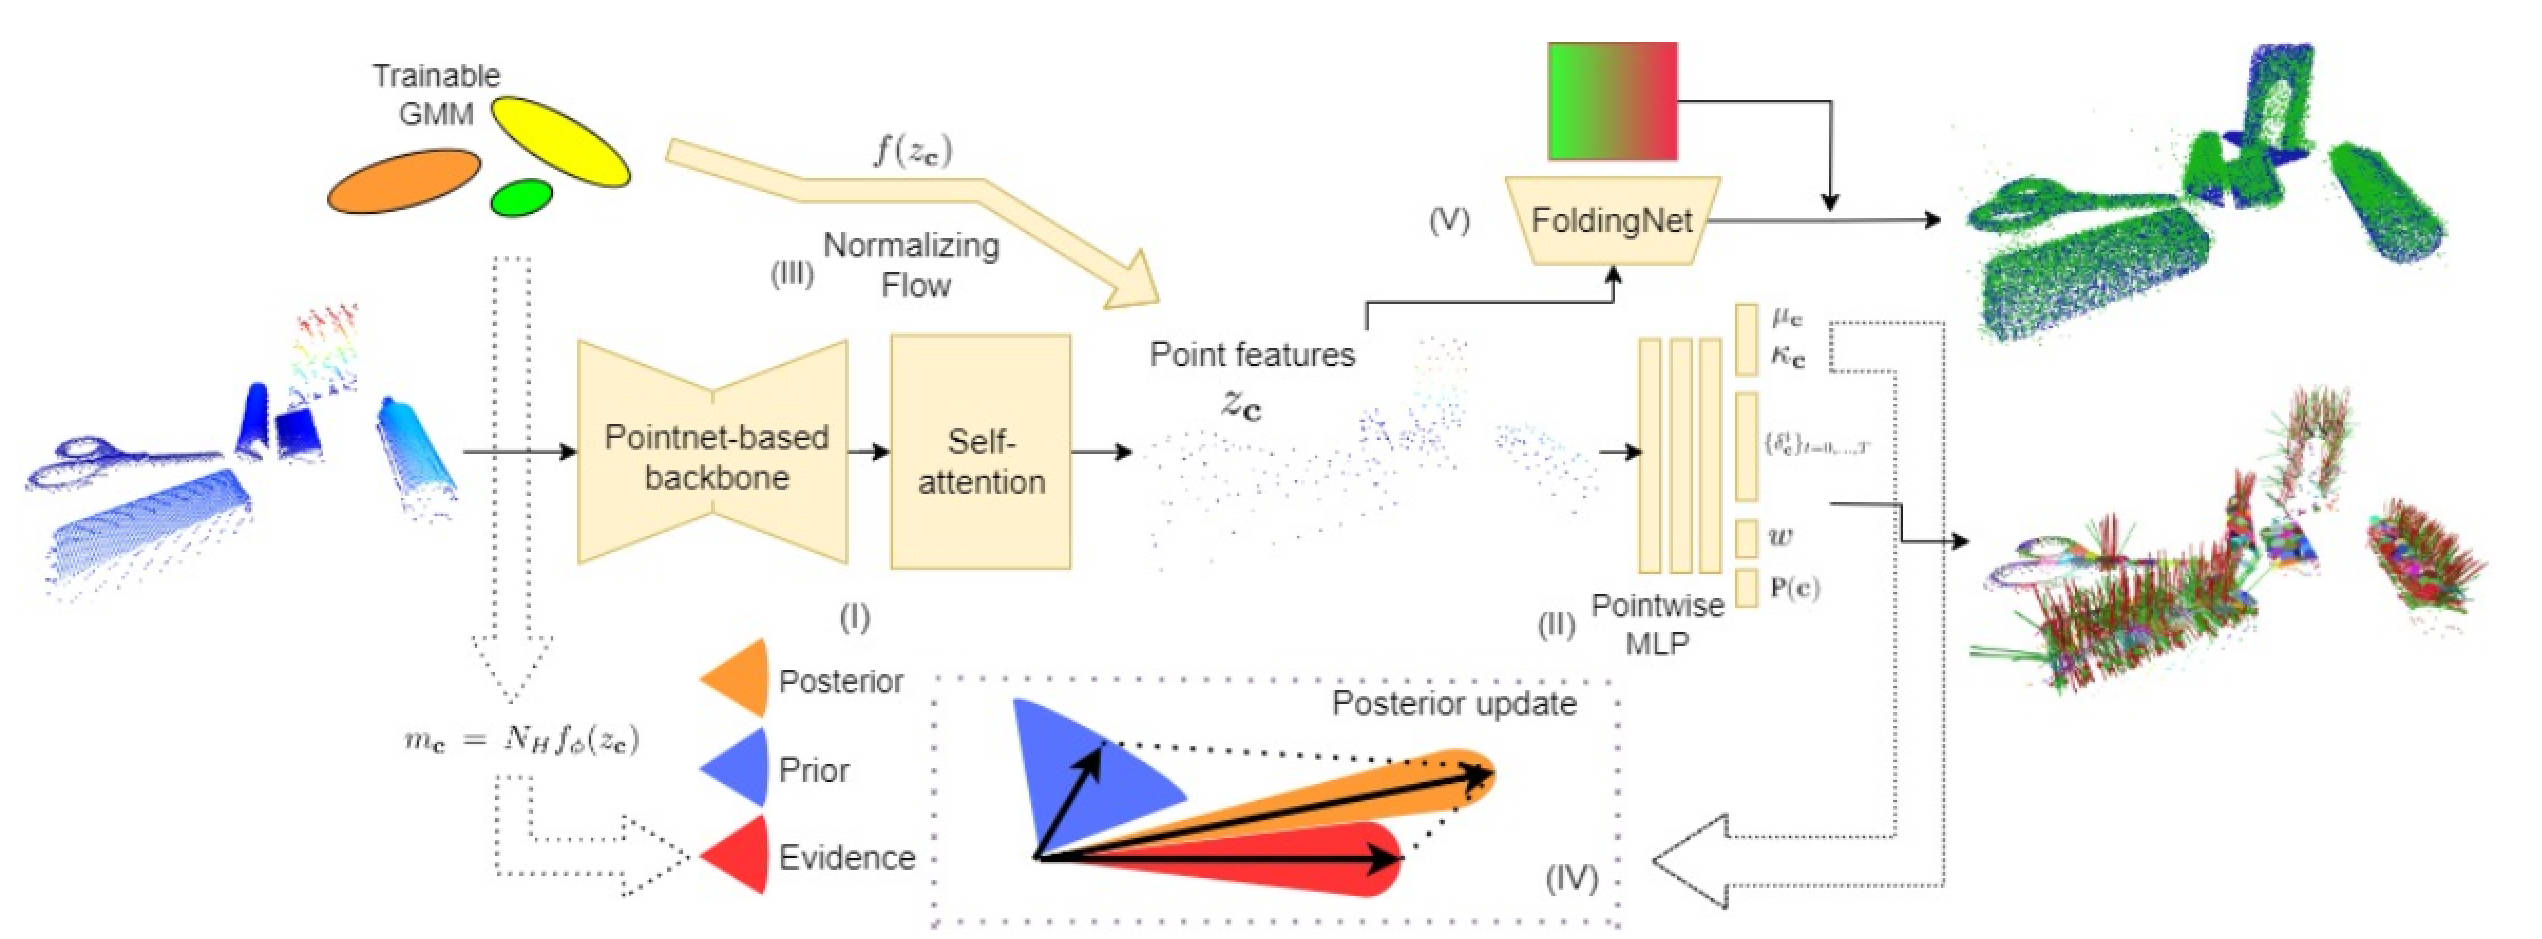
\includegraphics[width=1.0\textwidth]{vmf-architecture.jpg}
  \caption{An overview of the vMF-Contact architecture. Source: Adapted from \cite{shi2025}}
  \label{fig:vmf-architecture}
\end{figure}

vMF-Contact~\cite{shi2025} is this thesis's grasp generation component (\cref{sec:system-overview}). It embeds uncertainty directly into its generative model. An overview of its architecture is shown in \cref{fig:vmf-architecture}. It does not attach a post-hoc uncertainty estimator. Its foundation is the von Mises-Fisher distribution~\cite{fisher1953dispersion}. That distribution suits directional data on the unit hypersphere. vMF plays the role Gaussians play for scalar data. It gives a natural concentration parameter and max-entropy interpretation. This suits modelling contact normals, which are directional quantities.

% vMF-Contact models a distribution of contact normals, not one pose. Candidates are sampled from this distribution by probability mass. This captures aleatoric uncertainty from sensor noise and occlusion. It also captures epistemic uncertainty from limited training coverage. Low-density regions in the output mark low-confidence predictions.

% The result is a ranked candidate set with quantified confidence. 

% Rare training orientations occur in this thesis's 8-orientation matrix. For these, the predicted distribution turns broad and low-density. That signals high epistemic uncertainty at those orientations. Few or no candidates then survive post-processing filters (failure mode F2, \cref{chap:experimental-setup-and-results}). So the method fails detectably, never silently. This epistemic signal is vMF-Contact's most useful advantage.

\cite{shi2025} report 72.7\,\% success on a diverse-object benchmark. They used a Robotiq 2F-85 gripper and objects up to $\sim$1\,kg. Success there means isolated grasp detection only. It only checks whether the gripper closes stably. The benchmark excludes transport, placement, and downstream task success.

\section{The Industrial Deployment Gap}
\label{sec:industrial-deployment-gap}

Strong benchmarks do not guarantee reliable industrial deployment. The Amazon Picking Challenge~\cite{correll2016analysis} was an early structured real-world test. It involved picking from cluttered, variably lit shelves. Benchmark success did not always mean real-world reliability. This made deployment evaluation its own research concern.

The sim-to-real gap is a major contributor here. \cite{cai2024} flag real depth-sensor drift and deformation as key obstacles. Synthetic training data does not capture these sensor artefacts. Point-cloud quality then degrades in ways labs cannot see. This gap is systematic, not a fixable calibration error. \cite{tobin2017domain} used domain randomisation to narrow the sim-to-real gap. They randomised lighting, texture, and placement during training. This needs careful distribution design to work well. Real sensor artefacts still are not fully addressed.

\cite{kleeberger2020survey} surveyed deployment challenges for learning-based grasping broadly. They catalogue sensor noise, workspace limits, and force mismatch. Object variability is another recurring failure mode. They flag one recurring gap in the field. Most published work tests under easier-than-real conditions. Few papers offer failure analyses for specific hardware pairings.

Deployment success is more than just sensor noise. vMF-Contact's~\cite{shi2025} 72.7\,\% benchmark differs from this deployment in three ways. First, the benchmark's Robotiq 2F-85 gripper delivers 235\,N. This thesis's Robotiq 2F-140 delivers only 125\,N, a 47\,\% drop. It was chosen for its wider jaw opening. Second, benchmark objects weigh up to $\sim$1\,kg. The angle grinder here weighs about $\sim$2\,kg instead. Third, the benchmark measures only isolated grasp success. This thesis measures full pick-transport-place success instead. That metric adds trajectory execution and placement accuracy. Each difference independently lowers the expected success rate.

% A search of IEEE Xplore and Google Scholar using the terms (\texttt{``UR10'' OR ``UR10e''}) AND (\texttt{``ROS~2'' OR ``ROS2''}) AND (\texttt{``grasping'' OR ``pick-and-place''}) AND (\texttt{``deployment'' OR ``real-world''}) over 2020--2026 returned no peer-reviewed work reporting a structured real-deployment evaluation of a learning-based grasping method on a UR10/UR10e platform in a real industrial cell. To the best of the author's knowledge, no published study has conducted such an evaluation with results stratified across a controlled orientation-and-position trial matrix and a full pick-transport-place success criterion. The absence is informative: the field's evaluation standard does not yet demand what industrial deployment requires.


\textbf{Gap A --- Missing geometric priors in vMF-Contact.} Learning-based methods encode local contact geometry only. They ignore object-level spatial priors entirely. vMF-Contact does not constrain grasp-point-to-centroid distance. It also does not constrain gripper-axis alignment. Asymmetric objects then cause systematic failures. Extremity grasps far from centroid cause grip force insufficiency. Misaligned axis grasps cause orientation inconsistency.

\textbf{Gap B --- Absence of systematic deployment evaluation.} The literature offers isolated grasp benchmarks only. It lacks structured deployment studies with failure mode analysis. It also lacks real hardware-object constraints as criteria. Downstream task success is rarely the primary criterion.

% This thesis addresses Gap~A with two contributions. Contribution~A adds centroid-based and axis alignment constraints to vMF-Contact inference. Contribution~B adds a custom designed fingertip targeting the dominant failure mode. Contribution~D addresses Gap~B with structured deployment evaluation. It uses a 6-position $\times$ 8-orientation $\times$ 3-repetition trial matrix. This runs across three experimental conditions on a real UR10e cell.


% ============================================================
\chapter{System Design and Methodology}
\label{chap:system-design}
% ============================================================

The centroid-based constraints introduced in this thesis operate as a post-inference filter on the candidate set produced by vMF-Contact. Candidates that fail the spatial or axis alignment criteria are discarded before the highest-ranked remaining candidate is passed to the motion planner. The custom fingertip is a hardware modification to the Robotiq 2F-140 that operates independently of the algorithm. Both adaptations target specific, identifiable failure modes observed during baseline deployment, and are evaluated end-to-end in the full pipeline. Their individual contributions are isolated through the three-condition experimental design described in \cref{chap:experimental-setup-and-results}.

% This chapter builds on the hardware and software fundamentals introduced in \cref{chap:fundamentals} and describes the algorithmic and hardware contributions of this thesis. Section~4.1 describes the perception pipeline. Section~4.2 presents the centroid-based constraint formulation. Section~4.3 describes the custom fingertip design. Section~4.4 describes the ROS2 and Docker integration pipeline.

\section{Perception Pipeline}
\label{sec:perception-pipeline}

\begin{figure}[htbp]
  \centering
  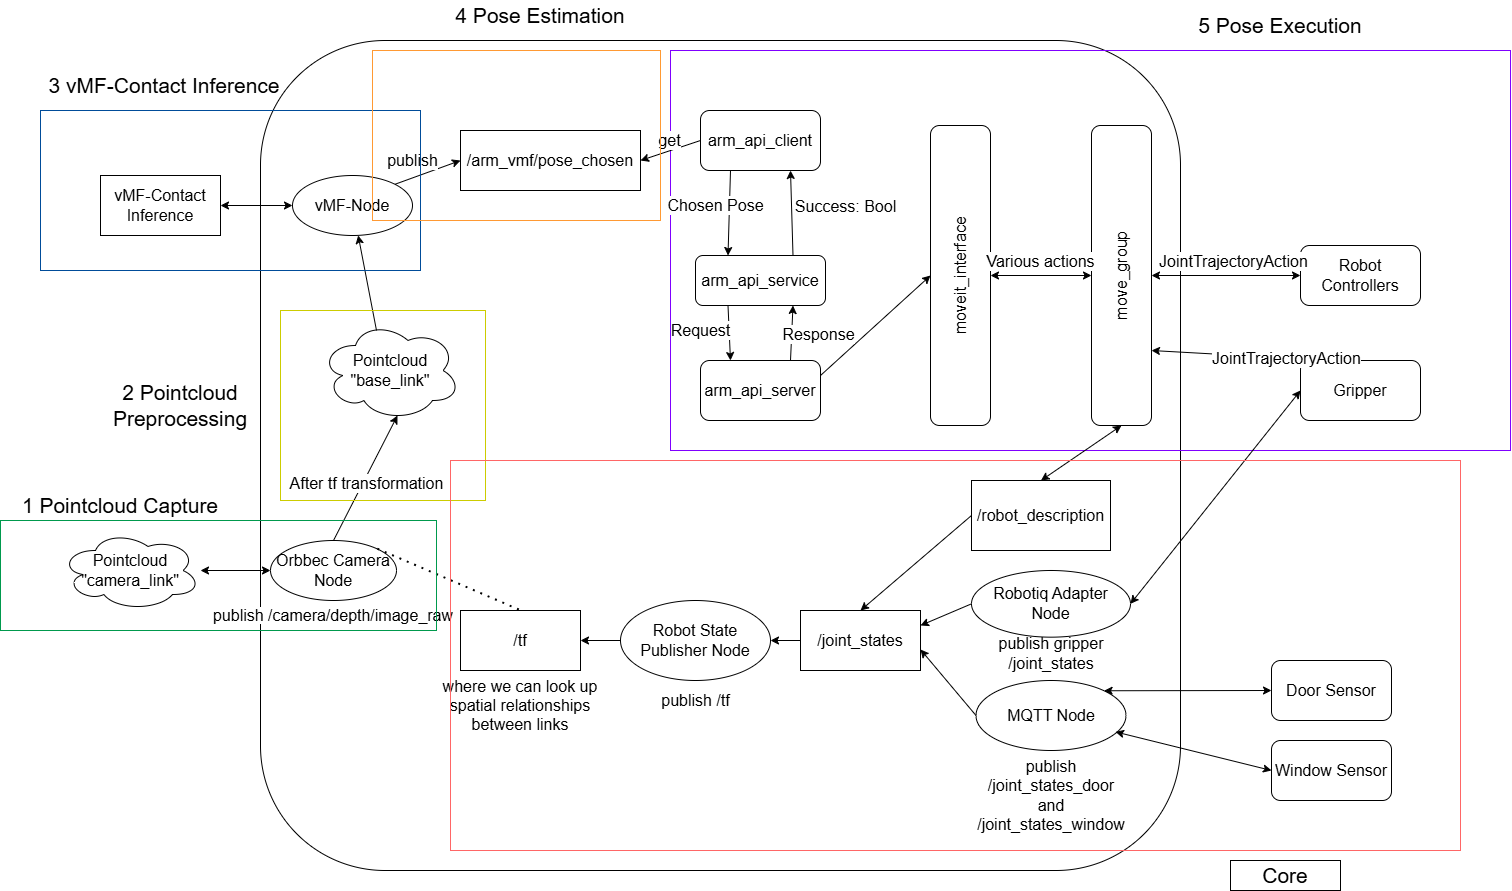
\includegraphics[width=1.0\textwidth]{vmf-pipeline.png}
  \caption{Inference-Perception-Execution pipeline overview. The pipeline proceeds from point cloud
    acquisition through centroid-filtered vMF-Contact inference, motion planning, and execution.}
  \label{fig:vmf-pipeline}
\end{figure}

The Orbbec Femto Mega streams RGBD frames at 10\,Hz. Each depth frame is converted to a point cloud in the camera optical frame and registered to the robot base frame using the calibrated static TF2 transform. The registered cloud is processed through a passthrough filter that restricts the sensing volume to the table surface region ($z$: -0.01--0.3\,m above base, $x$ and $y$: within the AGV delivery area). Point cloud noise is handled implicitly by the geometric centroid proxy (\cref{sec:centroid-distance-constraints}), With this kind of bounding-box limiting the observable point cloud, the algorithm can be more stable to sparse boundary noise. There is no separate outlier removal step in the pipeline.

The filtered point cloud is treated as a single-object scene. No instance segmentation step is applied before inference. This design reflects a constraint of the centroid-based filtering approach. The geometric centroid proxy used in the constraints (\cref{sec:centroid-distance-constraints}) is computed from the full filtered point cloud. In a multi-object scene, this operation would yield one average geometric centroid across all objects from the viewpoint, which would not be usable as filter criteria in further inference. Therefore, single-object placement within the delivery zone is a prerequisite of the current implementation. This scope boundary is discussed in \cref{sec:limitations}.

The preprocessed cloud is passed directly to the vMF-Contact inference module without additional voxelisation or surface normal pre-computation. The inference network handles these internally. It will publish the chosen grasp pose in ROS~2 topics after the inference. The Arm API client is always subscribed to this ROS~2 topic. Once a new grasp pose is published, it will send the request to the Arm API server. Ther Arm API server will then execute the target pose through moveit interface and UR robot. A "Gripper close/open" command will also be sent to the Robotiq 2f-140 gripper via URCaps. An overview of the inference-perception-execution pipeline is described in \cref{fig:vmf-pipeline}.

\section{vMF-Contact Inference and Centroid-Based Constraints}
\label{sec:vmf-contact-inference}

\subsection{Base Inference}
\label{sec:base-inference}

vMF-Contact~\cite{shi2025} takes the preprocessed point cloud as input and outputs a set of 6-DoF grasp candidates, each encoded as a $4\times4$ homogeneous transformation matrix in the camera frame. Candidates are generated by sampling contact normals from learned von Mises-Fisher distributions over the object surface and constructing gripper approach vectors accordingly. Each candidate carries a confidence score reflecting the probability mass of the underlying distribution at that contact location: high confidence indicates a contact normal consistent with the training distribution; low confidence indicates a contact geometry the model has limited exposure to.

In the unconstrained baseline (Baseline~1), the highest-confidence candidate is passed directly to the motion planner. No spatial or geometric post-processing is applied beyond the network's internal candidate ranking. This is the standard inference procedure as described in~\cite{shi2025}.

\subsection{Centroid Distance Constraints}
\label{sec:centroid-distance-constraints}

\begin{figure}[htbp]
  \centering
  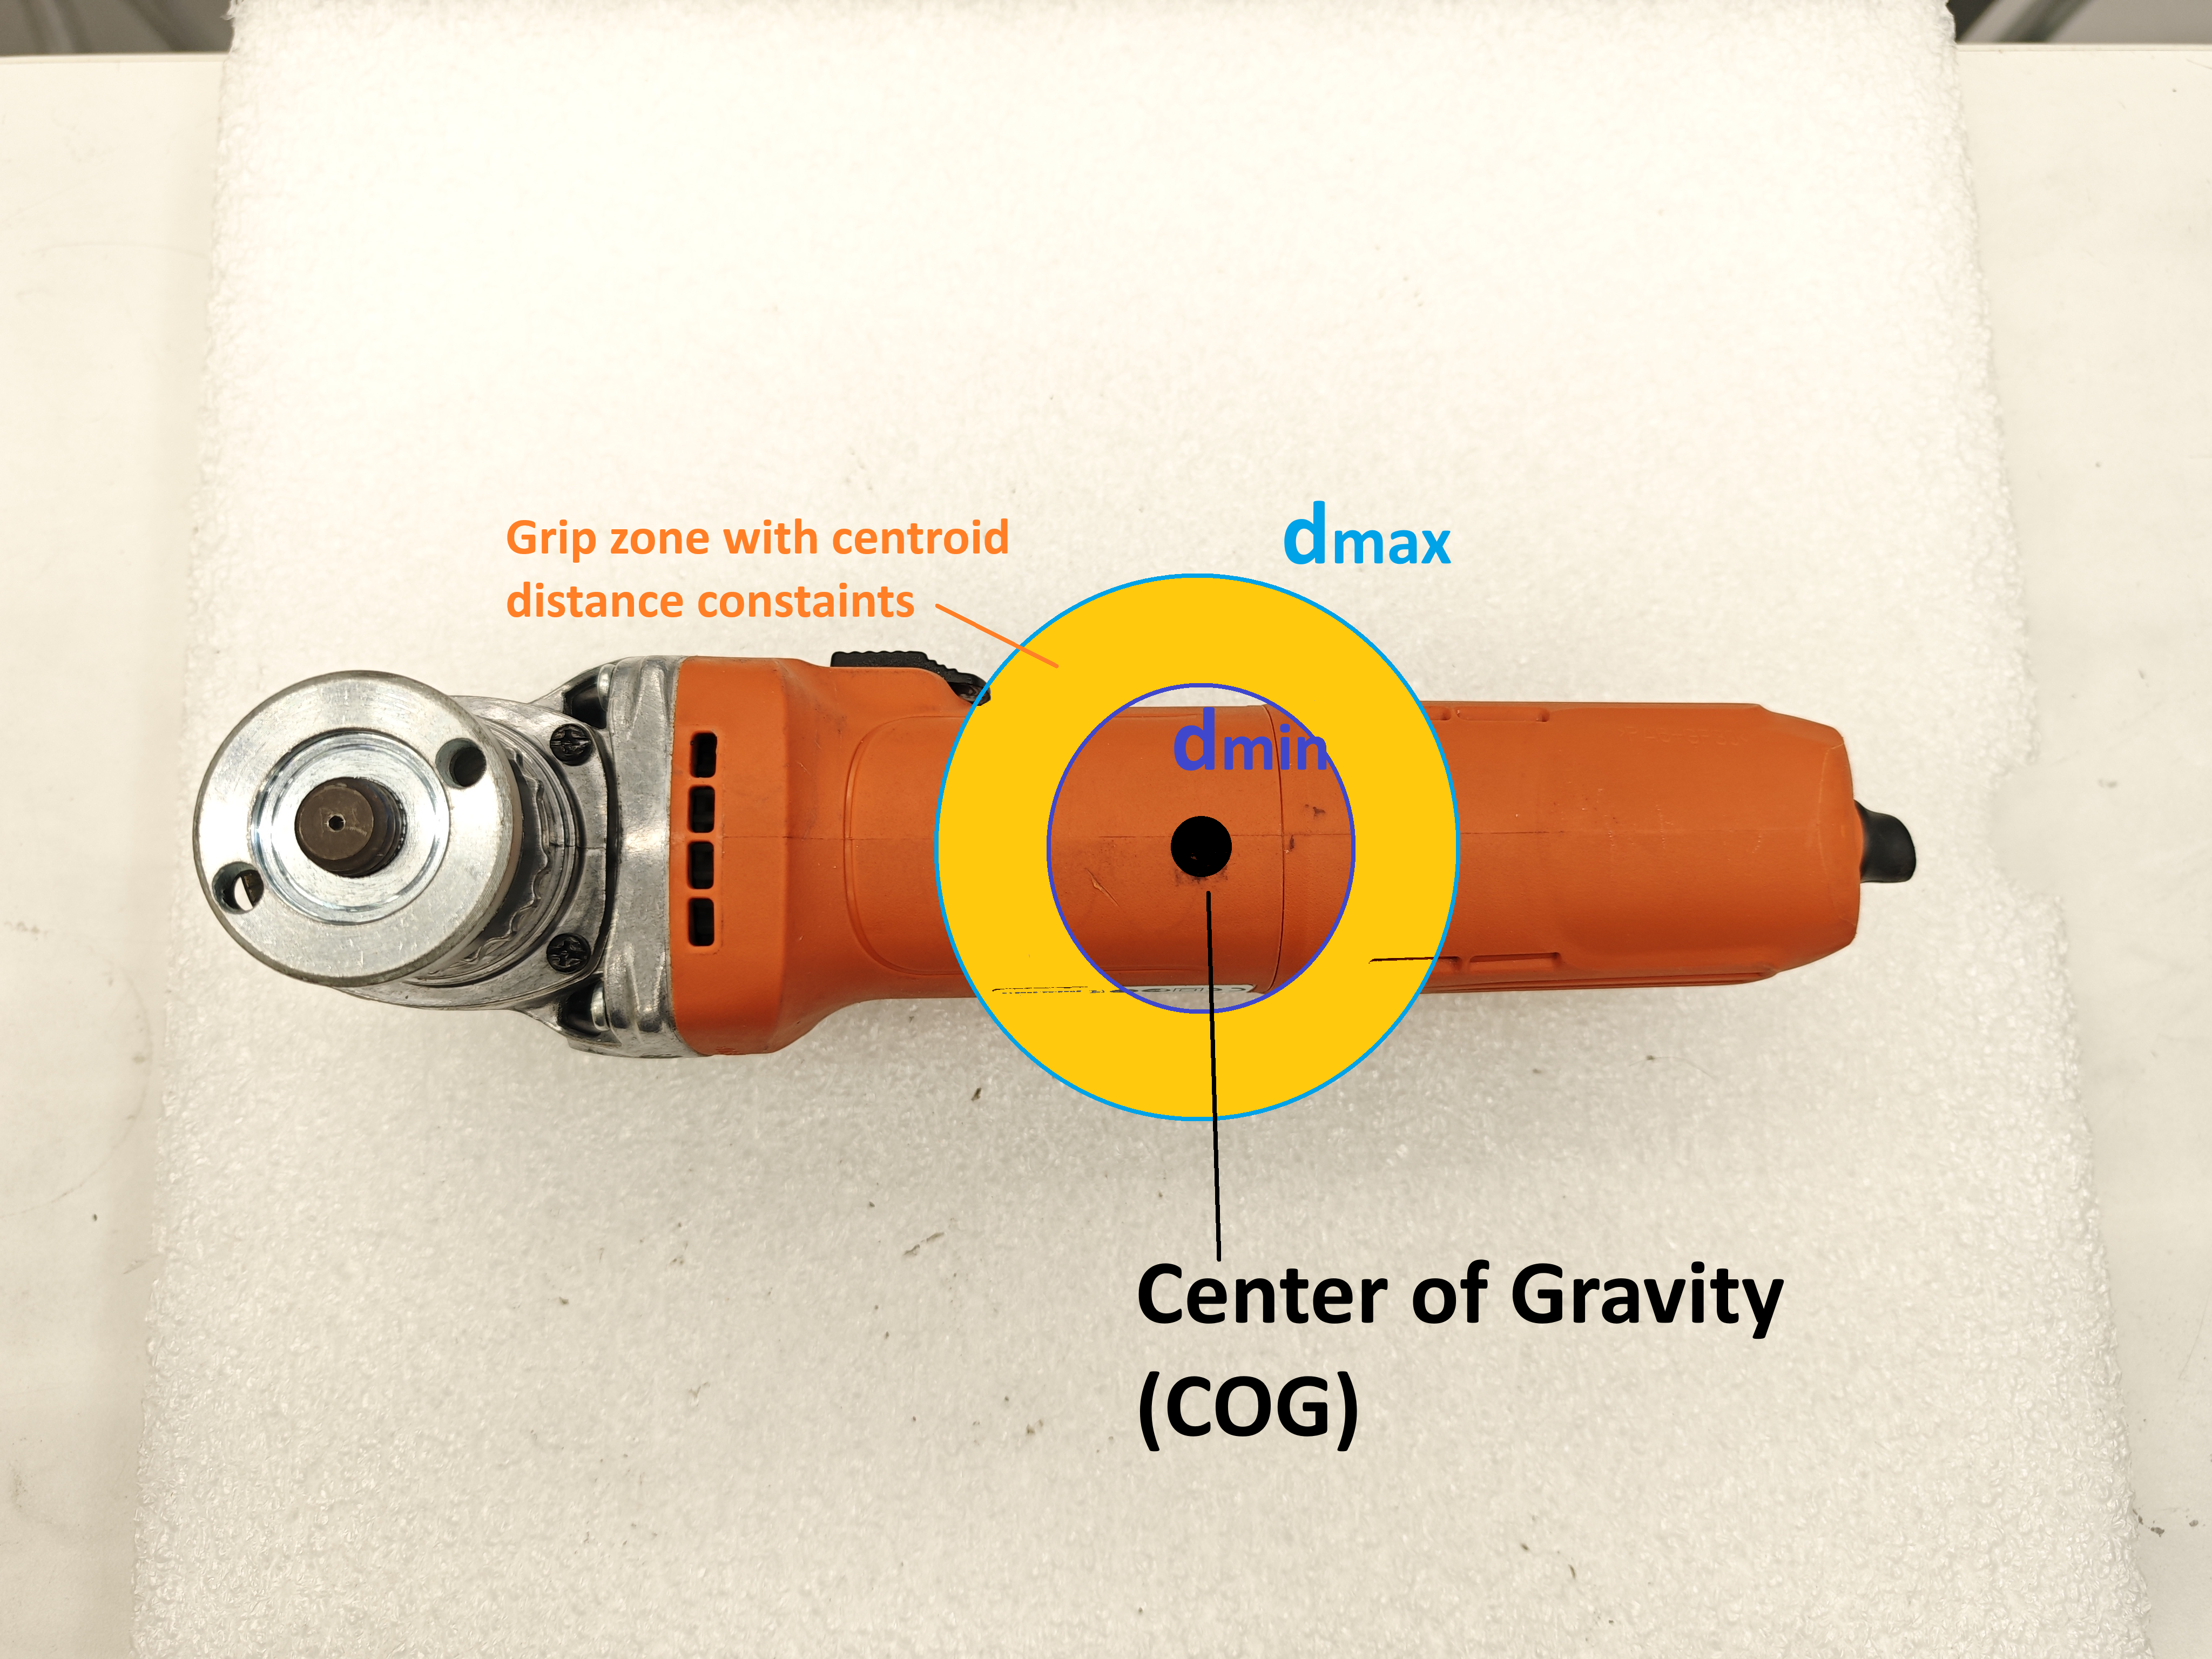
\includegraphics[width=0.6\textwidth]{angle-grinder-spherical-grip-zone-cog.png}
  \caption{Centroid-based grip zone (Equation~\ref{eq:cog}). Candidates
    within the shaded annulus are retained; candidates outside are discarded.}
  \label{fig:grip-zone}
\end{figure}

Two distance thresholds are applied to the candidate set following base inference. For each candidate, the Euclidean distance from the proposed grasp point to the object's geometric centroid proxy is computed. Candidates outside the interval $[d_{\min}, d_{\max}]$ are discarded.

The geometric centroid proxy is computed as a weighted sum of two point cloud statistics:

\begin{equation}\label{eq:cog}
  \hat{c} = 0.2 \cdot c_{\mathrm{obb}} + 0.8 \cdot c_{\mathrm{pcd}}
\end{equation}

where $\hat{c}$ is the geometric centroid proxy, $c_{\mathrm{obb}}$ is the centre of the object's oriented bounding box, and $c_{\mathrm{pcd}}$ is the centroid of the filtered point cloud. The 0.8 weighting towards the point cloud centroid reflects that the measured surface distribution provides a closer approximation to the object's mass distribution than the bounding box centre for an asymmetric object; the 0.2 bounding box contribution acts as a regulariser, stabilising the estimate against sparse or noisy boundary points where the raw point cloud centroid shifts toward the sensor-visible surface. This weighting was validated against the angle grinder's physical geometry by confirming that the resulting centroid proxy fell consistently within the mechanically stable grip zone across all five object positions. This approximation is a geometric proxy for the centre of gravity, not a physical measurement of it; it is referred to throughout this thesis as the \textit{geometric centroid proxy}.

The threshold values applied in this work are:
\begin{itemize}
  \item $d_{\max}$ = \param{grasp\_cog\_max\_dist\_th} = 0.025\,m (outer bound)
  \item $d_{\min}$ = \param{grasp\_cog\_min\_dist\_th} = 0.01\,m (inner bound)
\end{itemize}

These define a grip zone centred on the centroid proxy (\cref{fig:grip-zone}). Candidates beyond 0.025\,m or within 0.01\,m are rejected to prevent grip force insufficiency caused by excessive moment arm. The threshold values are geometrically motivated: the angle grinder's handle midpoint lies approximately 20\,mm from the centroid proxy, placing it within the $[0.01, 0.025]$\,m annulus. They were validated against the physical geometry of the object and are not the result of optimisation over trial outcomes. Their object-specificity is a stated limitation, discussed in \cref{sec:limitations}.

\subsection{Axis Alignment Constraint and Reachability}
\label{sec:axis-alignment-constraint}

A third filter enforces alignment between the gripper closing axis ($y$-axis in the gripper frame, projected into the object frame) and the object's principal axis (\cref{fig:axis-alignment}). The principal axis is the eigenvector corresponding to the largest eigenvalue of the point cloud covariance matrix. For each surviving candidate, the dot product between the projected gripper $y$-axis and the principal axis is computed; candidates below the threshold $th_{axis\_proj}$ (\param{cog\_axis\_projection\_th}) are discarded.

\begin{figure}[htbp]
  \centering
  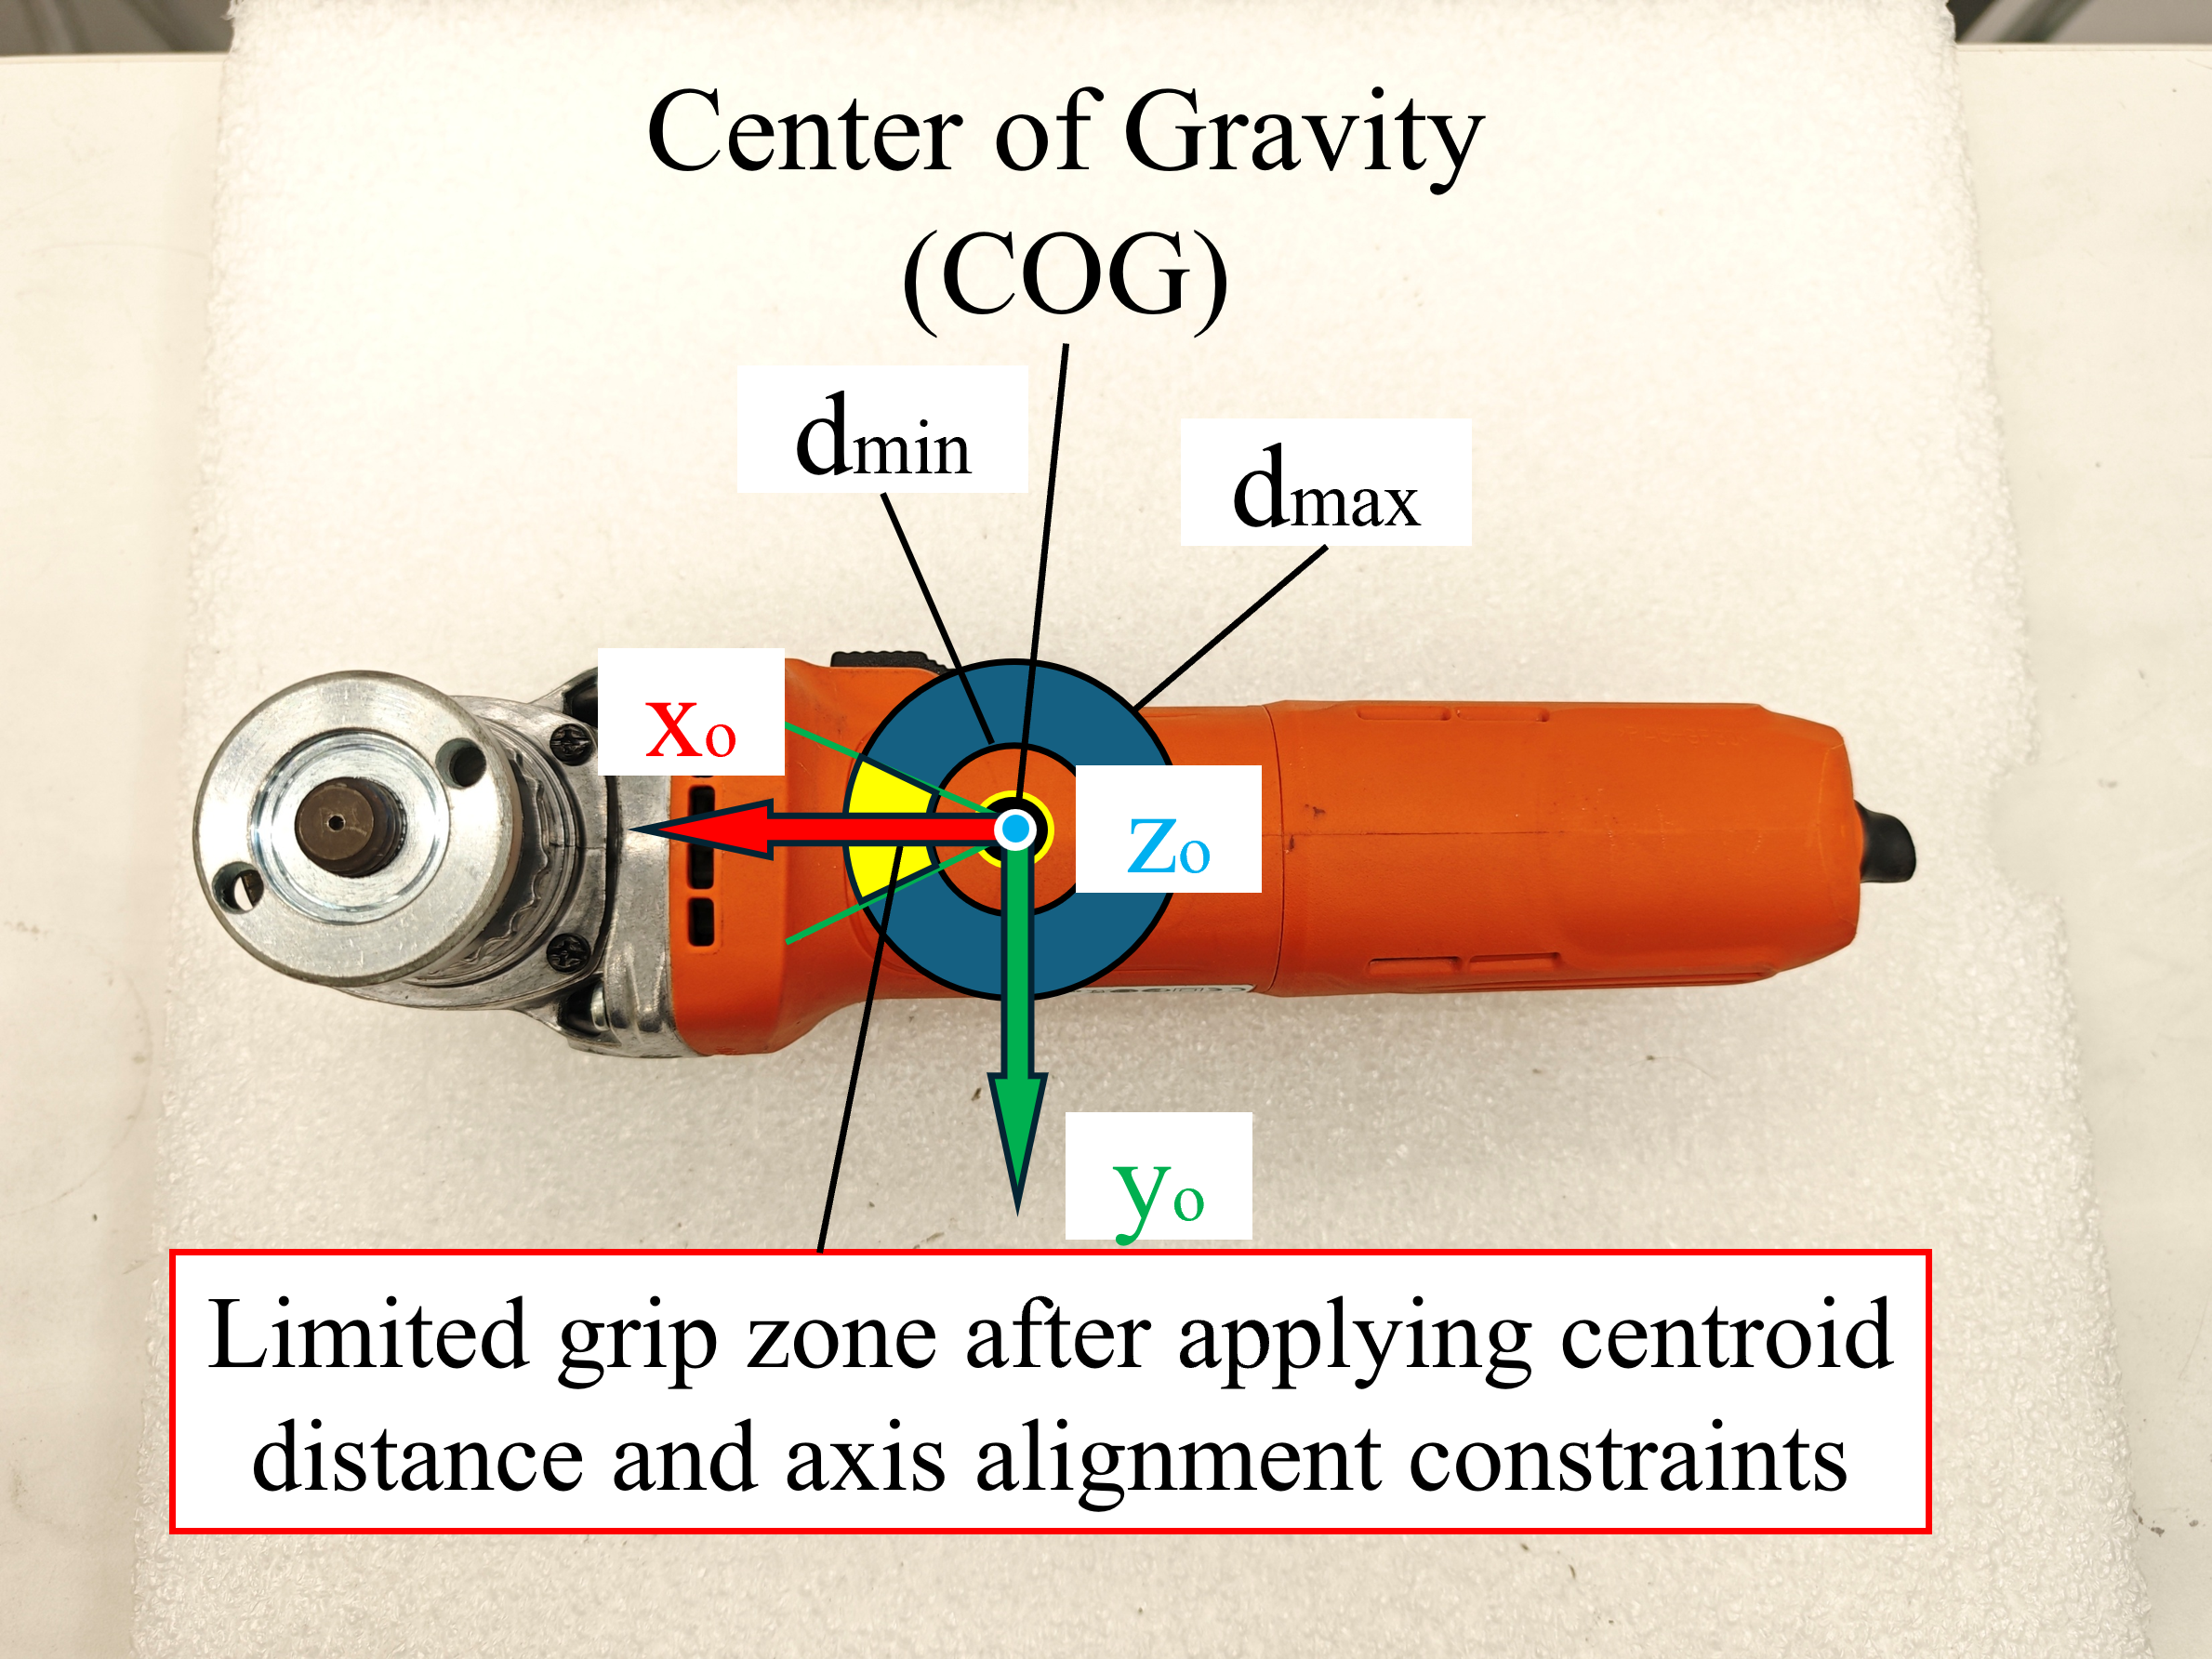
\includegraphics[width=0.6\textwidth]{angle-grinder-spherical-grip-zone-axis-caption.png}
  \caption{Axis alignment constraint. The gripper closing axis is
    constrained to align with the object's principal axis to avoid orientation errors.}
  \label{fig:axis-alignment}
\end{figure}

The three-filter cascade --- centroid distance inner bound, centroid distance outer bound, and axis projection --- constrains candidates to positions that are mechanically sufficient and orientationally consistent, addressing grip force insufficiency and orientation errors. It does not evaluate whether the selected candidate is kinematically reachable by the UR10e before committing to execution. A candidate that satisfies all three filters may still fail if the corresponding robot configuration falls outside the reachable workspace or violates joint limits. A fourth filter that evaluates kinematic reachability prior to final candidate selection --- pre-emptively discarding unreachable poses and selecting the next viable candidate --- is identified as a direction for future work (\cref{sec:future-work}) and implemented in Appendix \cref{sec:appendix-filter-design}.

\section{Custom Fingertip Design}
\label{sec:custom-fingertip-design}

The custom fingertip targets grip force insufficiency. It aims to address the problem, in which the gripper closes on a mechanically valid candidate within the centroid zone but releases the object during transport. The standard Robotiq flat fingertip contacts the angle grinder's cylindrical handle geometry at a single line of contact, producing minimal friction area and a low effective holding force relative to the object's weight.

The custom fingertip increases effective contact area through two design features. A curved contact surface, with a radius of curvature matched to the handle's cross-section ($\sim$20\,mm), converts the line contact of the flat fingertip to a surface contact, distributing grip force over a wider arc. A silicone friction layer (Shore~A~20 hardness, 8\,mm thickness) is bonded to the curved surface. The silicone is able to conform to surface irregularities on the handle. It can increase effective contact area and add additional gripping force to it. Together, these features raise the grip-to-weight margin at the same actuator force setting, without requiring any modification to the gripper controller or force parameters.

The fingertip improvement is isolated from the algorithm adaptation. It applies regardless of which algorithm generates the grasp candidate, provided the candidate is placed on the handle region. It is presented here as a necessary response to a hardware-object mismatch, not as a contribution specific to vMF-Contact or to learning-based grasping. The contribution of the thesis is the combined system, including the constrained algorithm and adapted hardware, evaluated end-to-end.

Fingertip bodies were fabricated by fused deposition modelling (FDM) in polyactic acid (PLA). Silicone was cast using a mold designed to fit in the recessed channel in the custom fingertip. The completed fingertips replace the standard pads on both jaws of the Robotiq 2F-140 without modification to the gripper's mechanical interface (\cref{fig:fingertip}).

\begin{figure}[htbp]
  \centering
  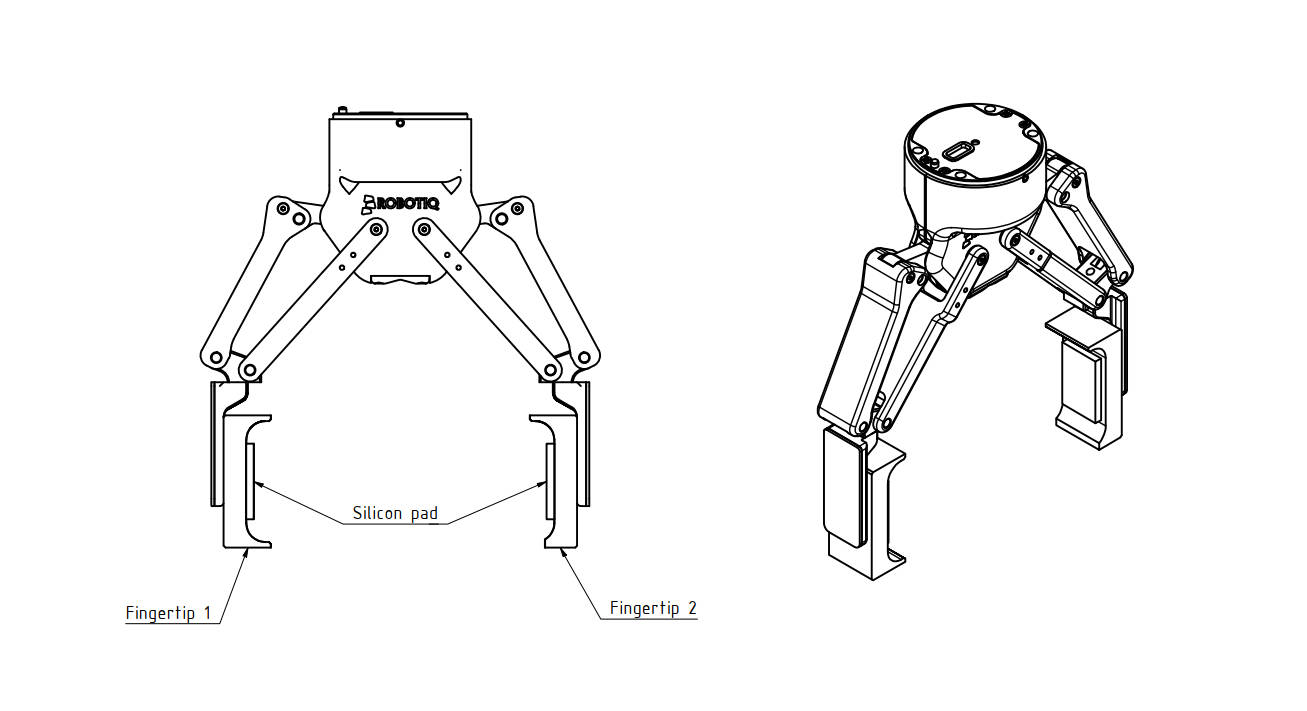
\includegraphics[width=0.95\linewidth]{fingertips.jpg}
  \caption{Custom fingertip. Left: design drawing. Right: installed on
    the Robotiq 2F-140.}
  \label{fig:fingertip}
\end{figure}

\section{ROS2 and Docker Integration Pipeline}
\label{sec:docker-configuration}

\begin{figure}[htbp]
  \centering
  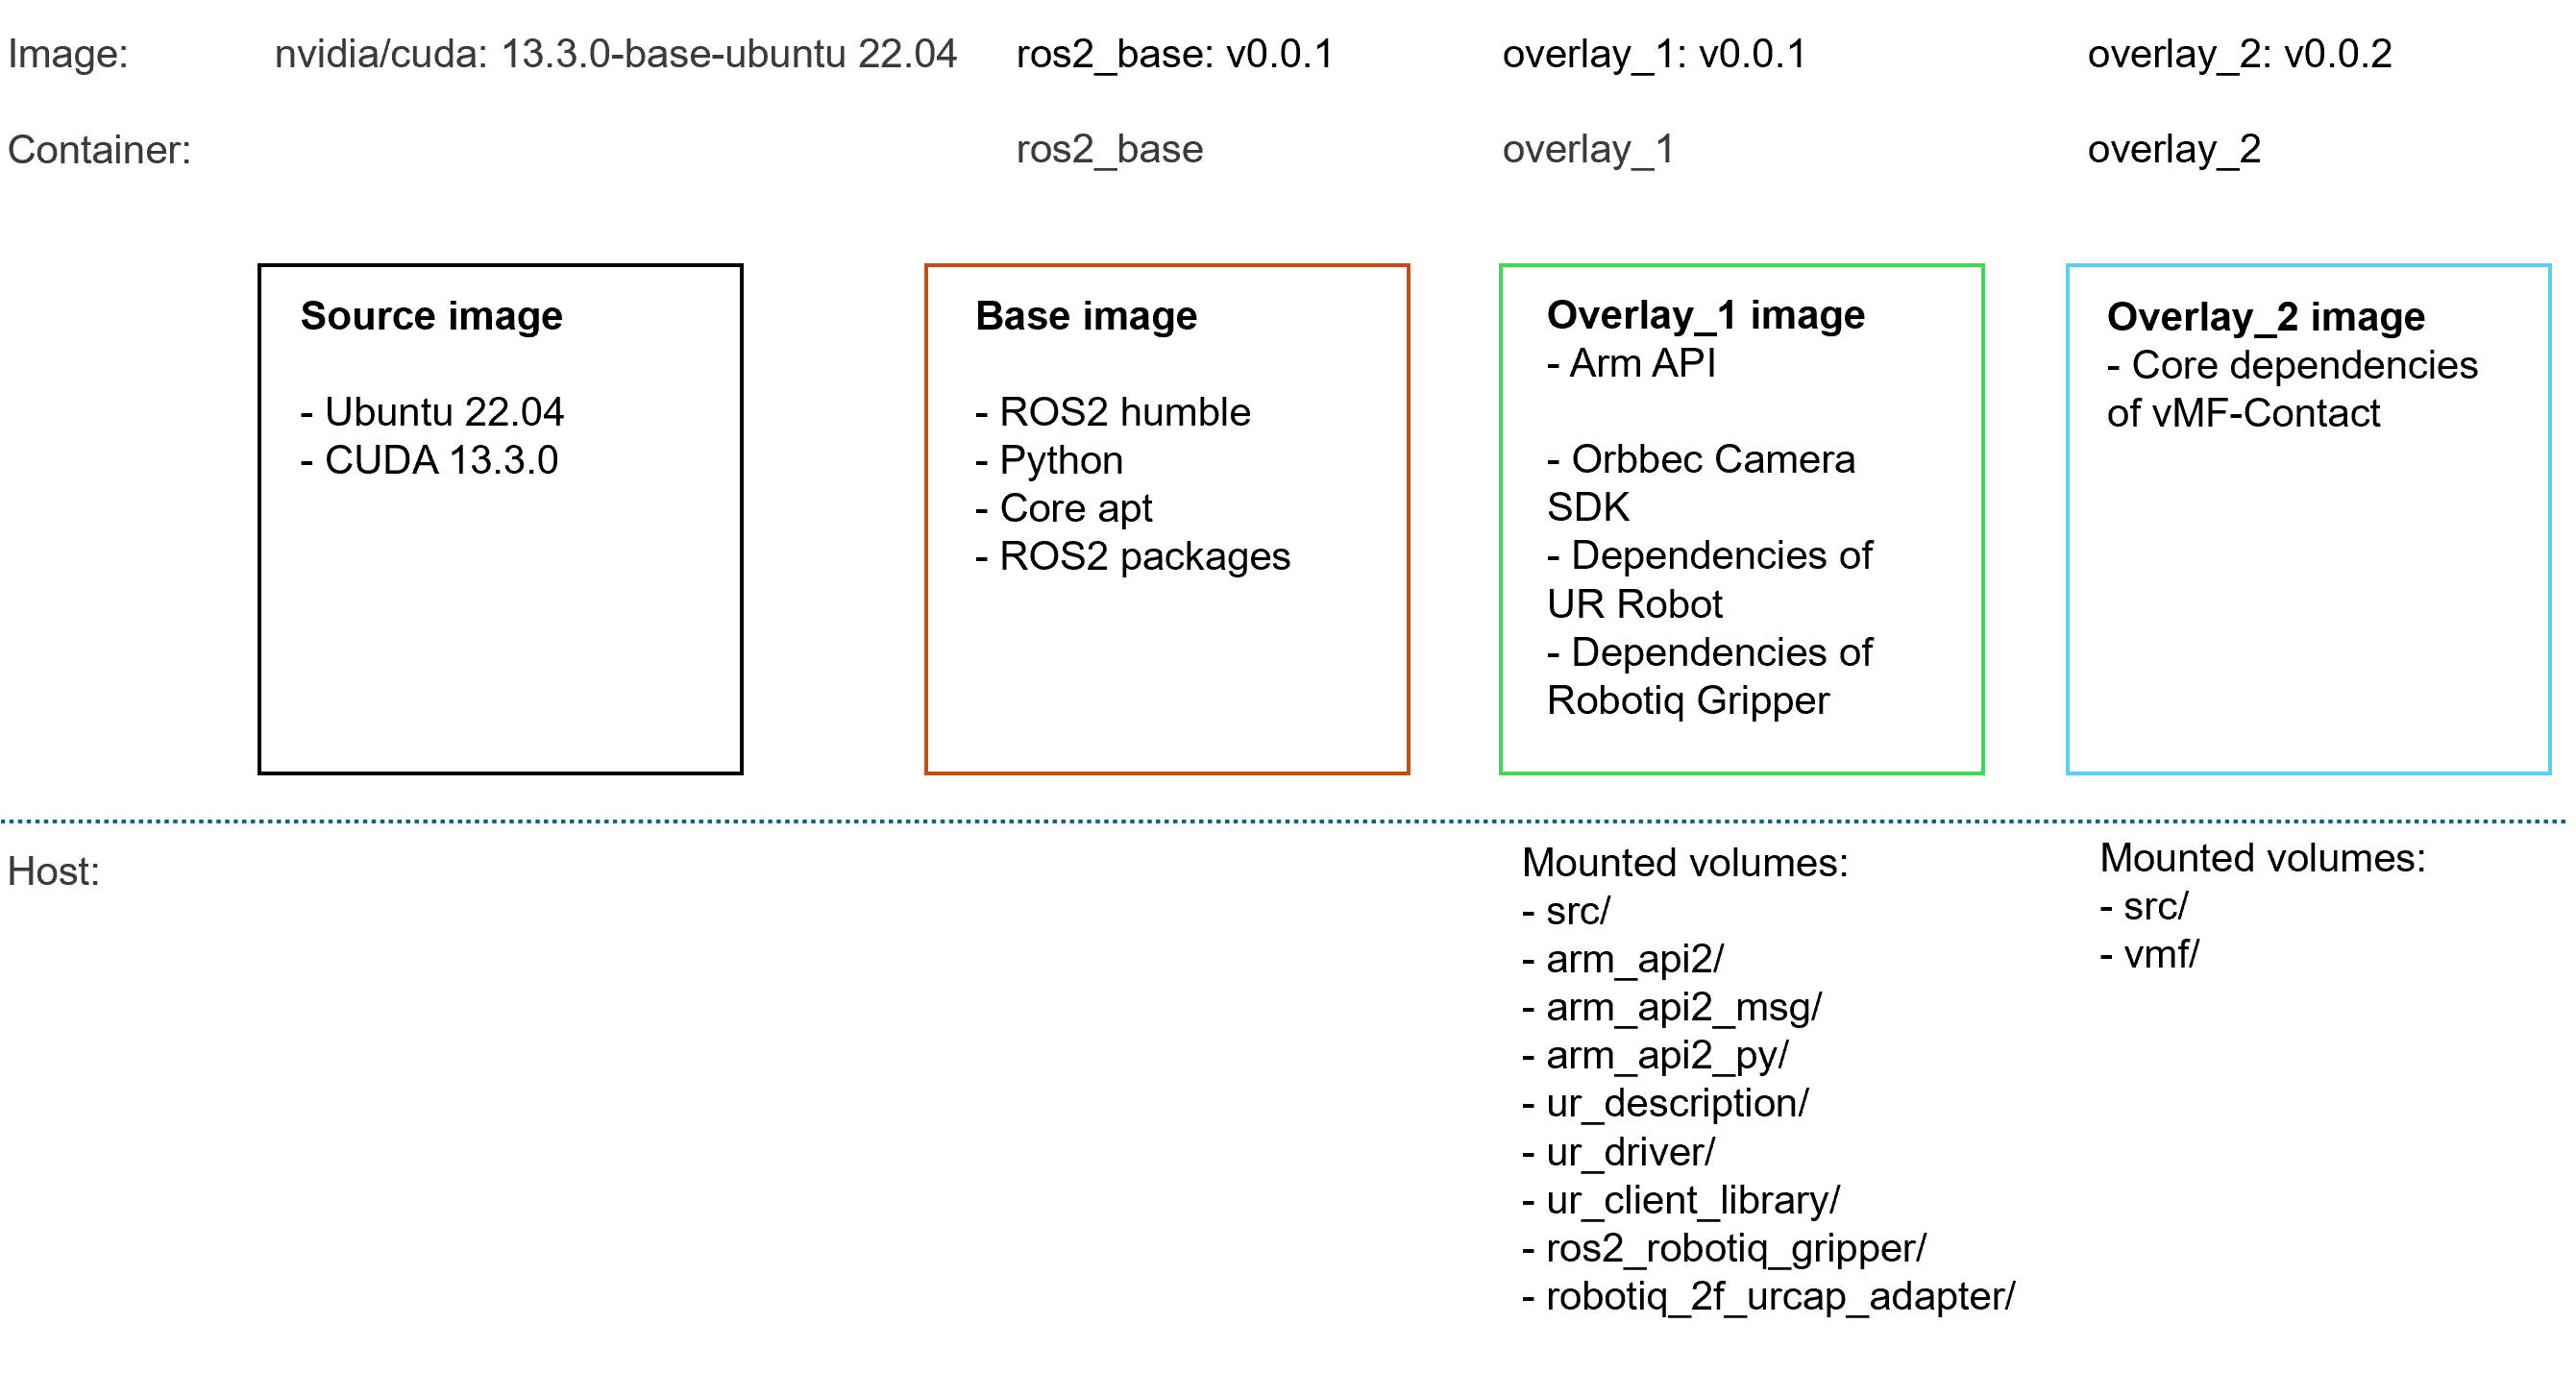
\includegraphics[width=0.95\linewidth]{docker-structure-full.png}
  \caption{Multi-layer docker container structure }
  \label{fig:docker-container-structure}
\end{figure}

The software stack runs on ROS2 Humble (Ubuntu 22.04) and is structured as 2 Docker containers managed by Docker Compose: perception (Orbbec ROS2 driver), inference (vMF-Contact, GPU-accelerated), motion planning (MoveIt~2 with UR10e model), and robot control (UR ROS2 driver), as shown in \cref{fig:docker-container-structure}. Containerisation includes all dependencies and environment in a single docker image, enabling fast deployment across development workstations with a simple "docker compose up" command.

Containers communicate over ROS2's DDS middleware (FastDDS) on a shared host network namespace, maintaining ROS2 node discovery without inter-container bridging. It serves as the software fundamentals for the perception-inference-execution pipeline shown in \cref{fig:vmf-pipeline}. 

The perception node processes and passes the original point cloud to the subsequent preprocessing node. The preprocessing node converts the point cloud in to the robot base frame via TF-transformation and passes it down. The inference node subscribes, runs inference and constraint filtering, and publishes the selected grasp pose in the robot base frame. The motion planning node computes a collision-aware trajectory using the UR10e URDF. The robot control node executes the trajectory and reports execution status. A logging node, co-located in the inference node, records per-trial metadata for each attempt: inference time, geometric centroid proxy, grasp pose, candidate count before and after filtering and point cloud logging.

The total pipeline latency from point cloud acquisition to robot motion onset is 3--5\,seconds under nominal conditions, dominated by vMF-Contact inference and MoveIt~2 trajectory planning. End-to-end cycle time (from point cloud acquisition through robot motion completion and return to the home position) is approximately 2\,minutes. This is acceptable for the CT-cell's operational throughput of one part per inspection cycle. Higher-throughput applications would require inference optimisation (e.g., model quantisation or TensorRT conversion) or pipelined execution of inference and planning.

% The complete pipeline is available at: \url{https://github.com/SFB-Circular-Factory-WG-C/docker\_vmf\_ur10e}


% ============================================================
\chapter{Experimental Setup and Results}
\label{chap:experimental-setup-and-results}
% ============================================================

\section{Experimental Protocol}
\label{sec:experimental-protocol}

\begin{figure}[htbp]
  \centering
  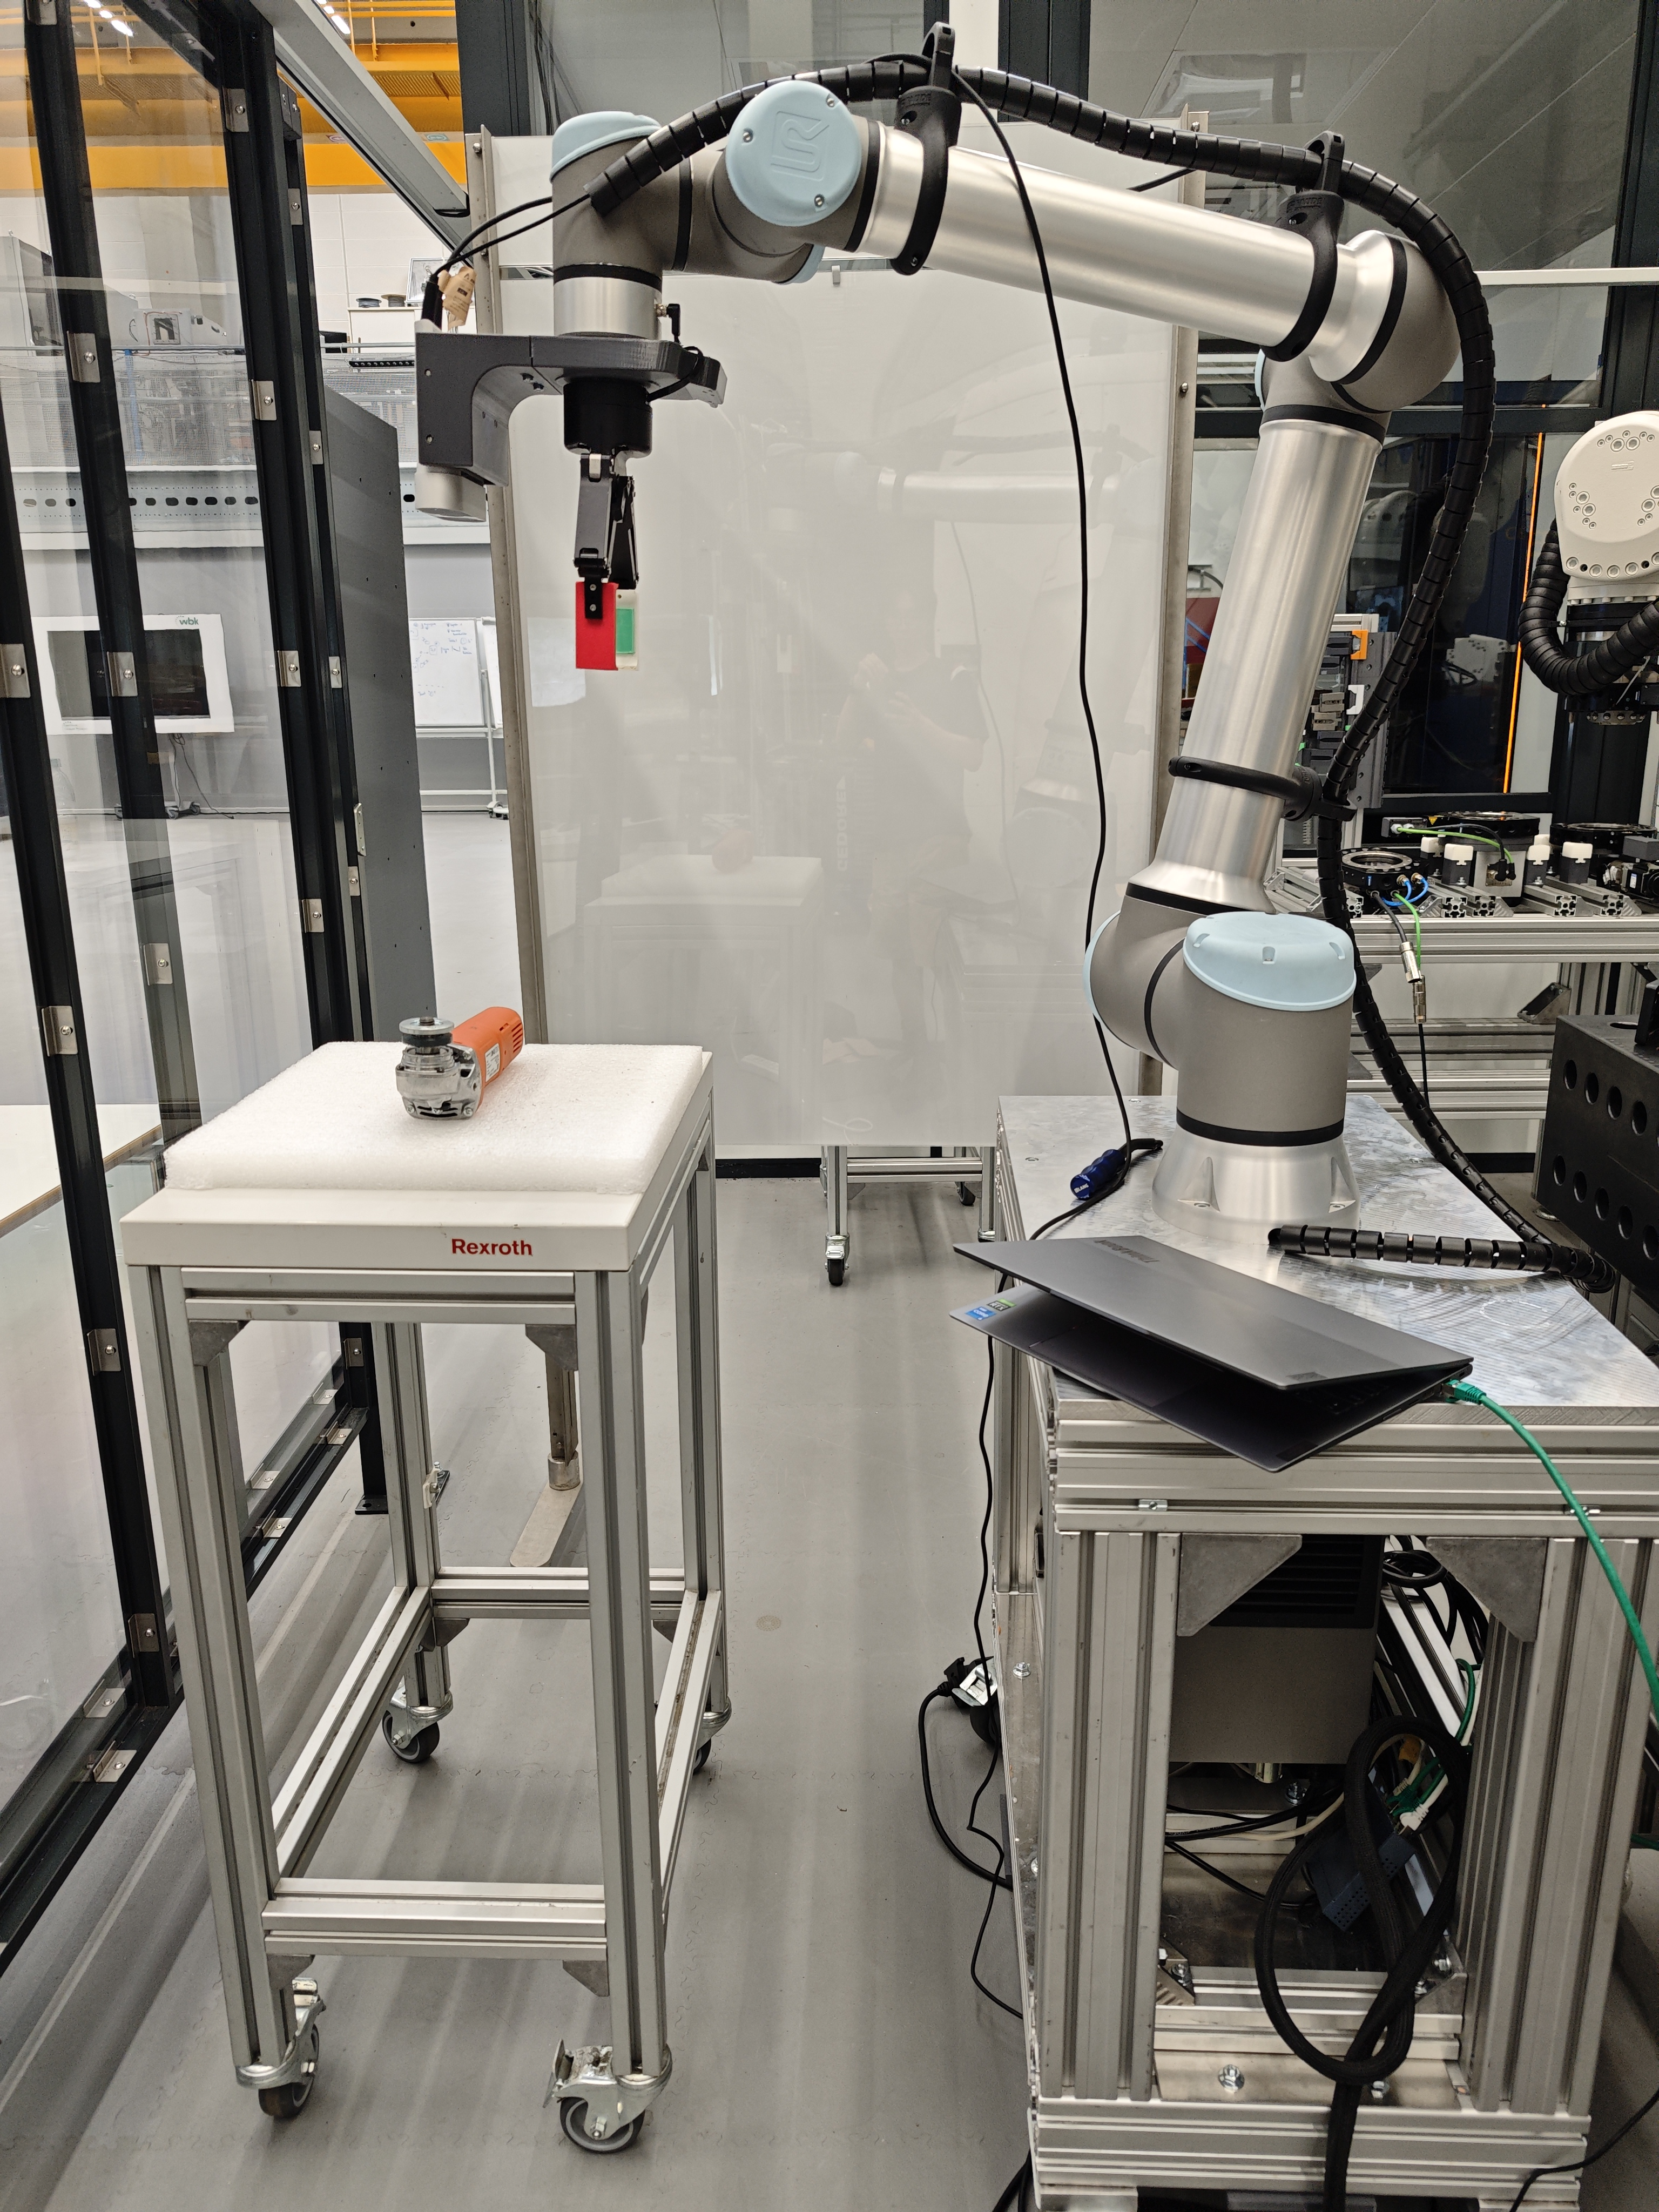
\includegraphics[width=0.8\textwidth]{robot-setup-1.jpg}
  \caption{Experimental setup. The UR10e is positioned to reach the
    AGV delivery zone, with the Orbbec Femto Mega mounted overhead. The angle grinder is placed at one of six positions and one of eight orientations for each trial.}
  \label{fig:exprimental-setup}
\end{figure}

\subsection{Trial Matrix}
\label{sec:trial-matrix}

\begin{figure}[htbp]
  \centering
  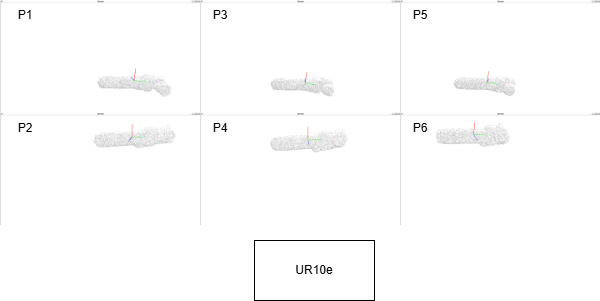
\includegraphics[width=0.95\linewidth]{pos-1-markup.png}
  \caption{6 object positions P1--P6 used in the evaluation.}
  \label{fig:pos-overview}
\end{figure}

\begin{figure}[htbp]
  \centering
  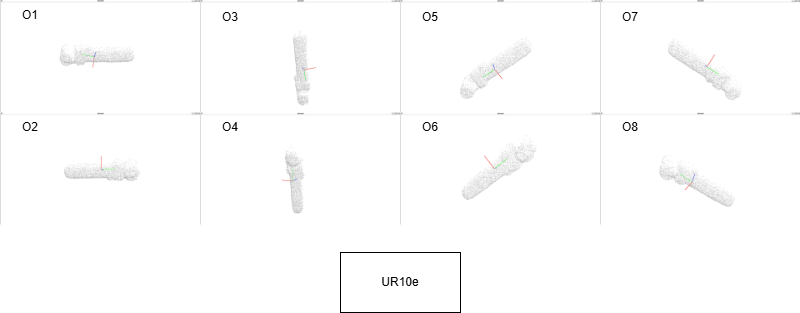
\includegraphics[width=0.95\linewidth]{orientation-D-markup.png}
  \caption{8 object orientations O1--O8 used in the evaluation.}
  \label{fig:orient-overview}
\end{figure}

The evaluation is structured as a $6 \times 8 \times 3$ factorial matrix: six object positions, eight object orientations, and three repetitions per cell, yielding 144 trials per experimental condition. All trials are conducted on the UR10e + Orbbec Femto Mega + Robotiq 2F-140 cell described in \cref{chap:fundamentals} and shown in \cref{fig:exprimental-setup}, under three conditions:

\begin{itemize}
  \item \textbf{Baseline~1:} vMF-Contact inference without centroid-based constraints, with the original Robotiq flat fingertip.
  \item \textbf{Baseline~2:} vMF-Contact inference with centroid-based and axis alignment constraints $d_{\max}$ = 0.025\,m, $d_{\min}$ = 0.01\,m, $th_{axis\_proj}$ = 0.5, with the original Robotiq flat fingertip.
  \item \textbf{Final:} vMF-Contact inference with the same centroid-based and axis alignment constraints as Baseline~2, with custom curved silicone fingertips as described in \cref{sec:custom-fingertip-design}.
\end{itemize}

Baseline~1 versus Baseline~2 isolates the software contribution, holding hardware constant. Baseline~2 versus Final isolates the hardware contribution, holding the algorithm constant. This factorial structure ensures that each contribution is attributable to a single changed variable.

% Statistical inference is conducted at the condition level (144 trials per condition); cell-level success rates (3 repetitions per position-orientation cell) carry a 95\,\% confidence interval width of approximately $\pm$26 percentage points and should be interpreted as descriptive rather than inferential.

\subsection{Object Positions and Orientations}

The six object positions (P1--P6, \cref{fig:pos-overview}) span the AGV delivery zone reachable by the UR10e, distributed to cover the range of expected delivery offsets encountered in the circular factory cell. The eight orientations (O1--O8, \cref{fig:orient-overview}) sample the angle grinder's rotational space at approximately 45$^\circ$ intervals around the vertical axis, probing the full range of top-down approach angles available to the parallel-jaw gripper. These orientations include configurations in which the tool head faces toward and away from the robot, and intermediate diagonal angles. They were selected without exclusion of orientations suspected to be kinematically difficult, to ensure that the reported success rates reflect realistic deployment conditions rather than a curated subset.

For each (position, orientation) cell, the angle grinder is manually placed to the target configuration before each of the three repetitions by the experimenter. This ensures that each repetition reflects an independent sensing and inference cycle rather than repeated planning on a fixed input.

\subsection{Success Criterion}
\label{sec:success-criterion}

A trial is recorded as a success if the angle grinder is lifted from the delivery position and transported to the CT scanner placement zone without being dropped (\cref{fig:success-grasp}). Minor manual intervention is recorded as partial success and is also counted as success in the final success rate, providing that the object is not released during the transport and placed in the placement zone within the orientation and position tolerance(\cref{fig:partially-success-grasp}). The placement zone is an angle grinder holder as shown in \cref{fig:angle-grinder-holder-tolerance}.

\begin{figure}[htbp]
  \centering
  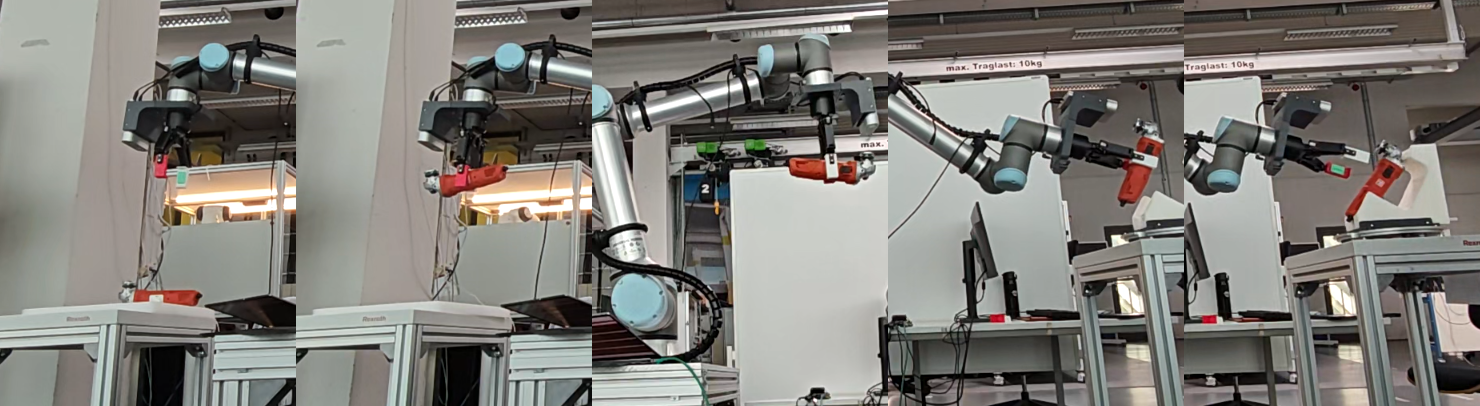
\includegraphics[width=0.95\linewidth]{success-grasp.png}
  \caption{Successful grasp. A grasp is counted as successful when the object is not released during the transport and placed in the holder within the orientation and position tolerance.}
  \label{fig:success-grasp}
\end{figure}

\begin{figure}[htbp]
  \centering
  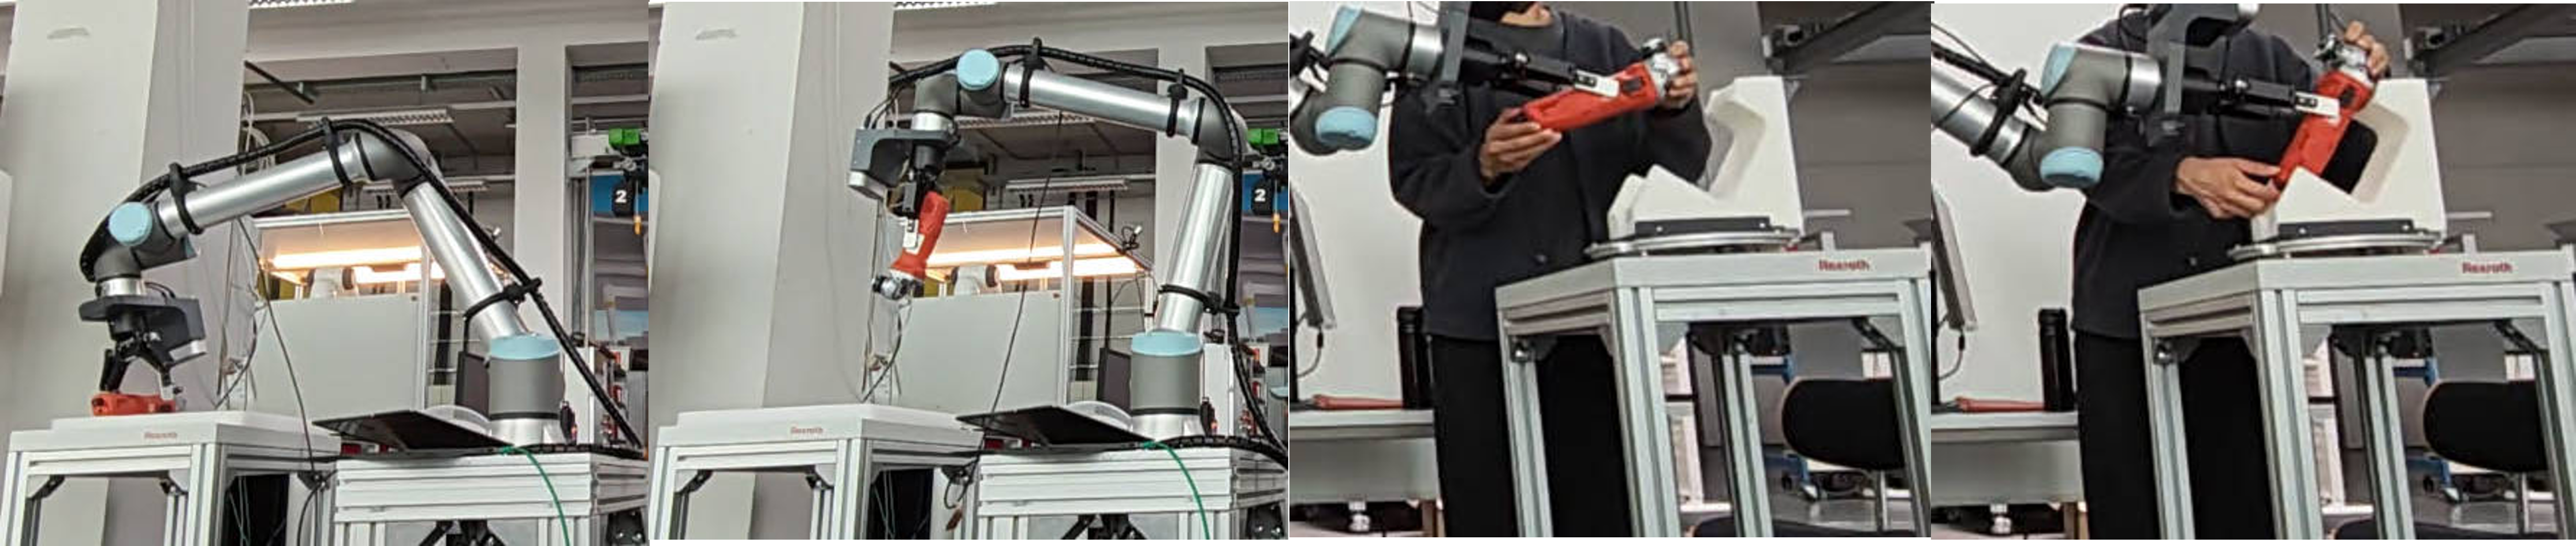
\includegraphics[width=0.95\linewidth]{partially-success-grasp.png}
  \caption{Partially successful grasp. Due to insufficient grip force,
    manual intervention is required during placement.}
  \label{fig:partially-success-grasp}
\end{figure}

\begin{figure}[htbp]
  \centering
  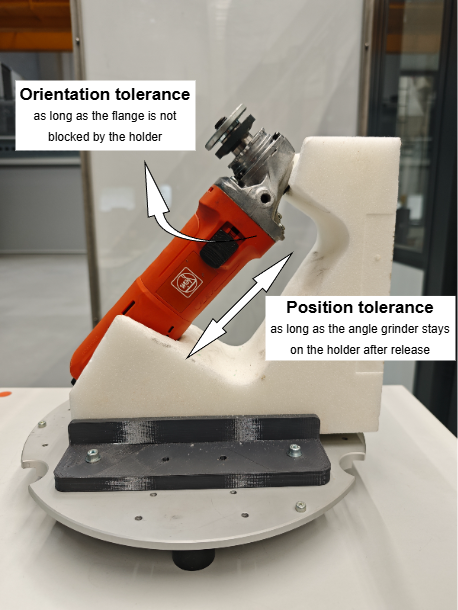
\includegraphics[width=0.4\linewidth]{angle-grinder-holder-tolerance.png}
  \caption{An angle grinder holder with the description of tolerance of placement.}
  \label{fig:angle-grinder-holder-tolerance}
\end{figure}

Trials in which the gripper closes but the object is released during transport (F1), in which no valid candidate is selected after filtering (F2), in which the motion planner does not find a feasible trajectory or the robot hits its joint limit during motion (F3), or in which the object arrives at the placement zone with an inverted orientation (F4) are recorded as failures. F1, F2, F3, and F4 are classified by failure mode in \cref{sec:failure-mode-definitions}. All 144 trials per condition are included in the reported success rate. No trials are excluded after data collection.

\section{Results by Condition}

\subsection{Condition Success Rates}
\label{sec:condition-success-rates}

Table~\ref{tab:success-rates} summarises the overall success rates for each condition across all 144 trials.

\begin{table}[htbp]
  \centering
  \caption{Overall success rates per condition (144 trials each).}
  \label{tab:success-rates}
  \begin{tabular}{llllr}
    \toprule
    Condition & Algorithm & Fingertip & Successes & Rate \\
    \midrule
    Baseline~1 & vMF-Contact (unconstrained) & Robotiq original &
      20 / 144 & 13.9\,\% \\
    Baseline~2 & vMF-Contact + CoG constraints & Robotiq original &
      58 / 144 & 40.3\,\% \\
    Final & vMF-Contact + CoG constraints & Custom silicone &
      111 / 144 & 77.1\,\% \\
    \bottomrule
  \end{tabular}
\end{table}

All three pairwise differences between conditions are statistically significant. $\chi^2$ tests of proportions ($df = 1$) yield: Baseline~1 vs.\ Baseline~2: $\chi^2 = 25.39$, $p < 0.001$; Baseline~2 vs.\ Final: $\chi^2 = 40.22$, $p < 0.001$; Baseline~1 vs.\ Final: $\chi^2 = 115.96$, $p < 0.001$. Using the confirmed approximate rates (13.9\,\%, 40.3\,\%, 77.1\,\%) as working estimates yields $\chi^2$ values of $\approx$14, $\approx$40, and $\approx$77 respectively, each far exceeding the $\chi^2(1)$ critical value of 10.83 at $\alpha = 0.001$.

This confirms that the observed improvements are not attributable to random chance and that both the algorithmic and hardware contributions are independently significant.

\subsection{Factorial Decomposition}
\label{sec:factorial-decomposition}

The Baseline~1 success rate of 13.9\,\% establishes that unconstrained vMF-Contact inference is not viable for this deployment. The algorithm generates geometrically plausible candidates that are mechanically or orientationally incompatible with the task at the large majority of tested conditions.

The transition from Baseline~1 to Baseline~2, which shows an improvement of 26.4 percentage points, represents the software contribution. Centroid-based constraints filter out candidates at object extremities and enforce axis alignment, directly addressing both dominant Baseline~1 failure modes. This improvement is attributable entirely to the algorithmic modification; hardware is held constant.

The transition from Baseline~2 to Final, which shows an improvement of 36.8 percentage points, represents the hardware contribution. The custom fingertip increases effective contact area and friction on the angle grinder handle, recovering grip failures on candidates that are algorithmically valid but mechanically marginal with the flat fingertip. This improvement is attributable entirely to the hardware modification; the algorithm is held constant.

Both contributions are independently load-bearing. As shown, the Baseline~2 result (40.3\,\%) is insufficient for reliable industrial operation. It shows that algorithmic contribution alone does not solve the deployment problem. A hypothetical custom-fingertip-only deployment without centroid constraints was not evaluated. The hardware contribution measured here (Baseline~2 to Final, showing an improvement of 36.8\,\%) is therefore conditional on the centroid-based constraints being active. It shows that both hardware and software contributions are necessary to achieve the Final condition's 77.1\,\% success rate. More implications of this result are discussed in \cref{sec:results-summary}.

\subsection{Benchmark Comparison}
\label{sec:benchmark-comparison}

The Final condition result of 77.1\,\% demonstrates viability under conditions more demanding than those of the vMF-Contact benchmark~\cite{shi2025} along three independently measurable axes:

(1)~the Robotiq 2F-140 grip force (125\,N) is 47\,\% lower than the 2F-85 (235\,N) used in the benchmark;

(2)~the angle grinder ($\sim$2\,kg) is approximately twice the weight of benchmark objects;

(3)~the success criterion encompasses the full pick-transport-place sequence, whereas the benchmark measures isolated grasp detection.

Each factor independently depresses the achievable success rate relative to the benchmark setting. That the Final condition achieves 77.1\,\% despite these three compounding disadvantages indicates that the centroid-based constraints and custom fingertip are sufficient to maintain above-benchmark performance even under substantially harder deployment conditions, not that the adapted system is intrinsically superior to the base algorithm on the benchmark task itself.

\section{Failure Mode Analysis}
\label{sec:failure-mode-analysis}

\subsection{Failure Mode Definitions}
\label{sec:failure-mode-definitions}

Four failure modes are defined:

\subsubsection{F1 (Grip force failure)}
The gripper closes and the trajectory executes, but the object is dropped during transport (\cref{fig:failure-mode-F1}). Detected by visual inspection.

The angle grinder weighs approximately 2\,kg and has an asymmetric elongated geometry. Grasps placed at the extremities of the object, either the tool head or the rear handle end, generate a torque about the gripper contact line proportional to the moment arm between the grasp point and the object's centre of gravity. At the Robotiq 2F-140's maximum grip force of 125\,N, this moment arm exceeds the stable holding threshold when the grasp is placed beyond approximately 50\,mm from the centroid.

The vMF-Contact network assigns candidate confidence based on local surface geometry (curvature, contact normal direction, antipodal compatibility) without reference to where on the object the candidate lies relative to its mass distribution. A geometrically valid contact normal at the tool head is assigned the same score basis as one near the handle centre. The base inference pipeline therefore offers no mechanism to preferentially select candidates in the mechanically stable region.

\begin{figure}[htbp]
  \centering
  \includegraphics[width=0.95\linewidth]{F1.png}
  \caption{Failure mode F1. Gripper failed to grasp the object.}
  \label{fig:failure-mode-F1}
\end{figure}

\subsubsection{F2 (No valid pose)}
No valid candidate is selected after filtering (\cref{fig:failure-mode-F2}). Detected by the inference node.

Following all three filters introduced in \cref{sec:centroid-distance-constraints} and \cref{sec:axis-alignment-constraint}, the remaining candidates are ranked by the original vMF-Contact confidence scores and the top-ranked candidate is passed to the motion planner. If no candidates survive, the inference node reports a no-valid-pose F2 failure without executing.

\begin{figure}[htbp]
  \centering
  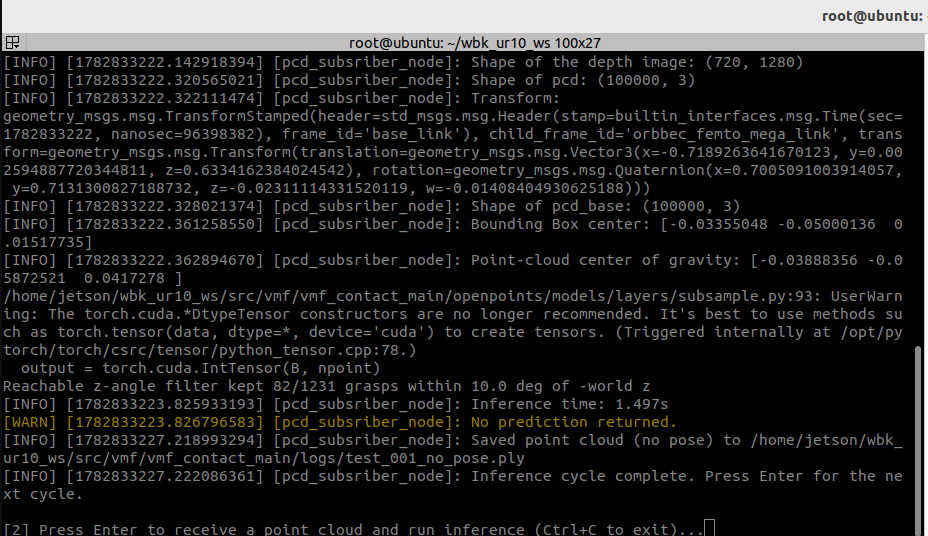
\includegraphics[width=0.95\linewidth]{F2.png}
  \caption{Failure mode F2: No valid candidate after filtering.}
  \label{fig:failure-mode-F2}
\end{figure}

\subsubsection{F3 (Kinematic infeasibility)}
A valid candidate is selected, but the MoveIt~2 planner fails to find a collision-free trajectory or certain joints exceed their limits (\cref{fig:failure-mode-F3}). Reported by the planning node or robot controller.

The robot cannot reach a pose that is orientationally valid, because the required joint configuration falls outside the UR10e's reachable workspace or violates joint limits. F3 failures are independent of the object's geometry or the algorithm's candidate quality; they are a function of the spatial relationship between the candidate pose and the robot's kinematic envelope.

\begin{figure}[htbp]
  \centering
  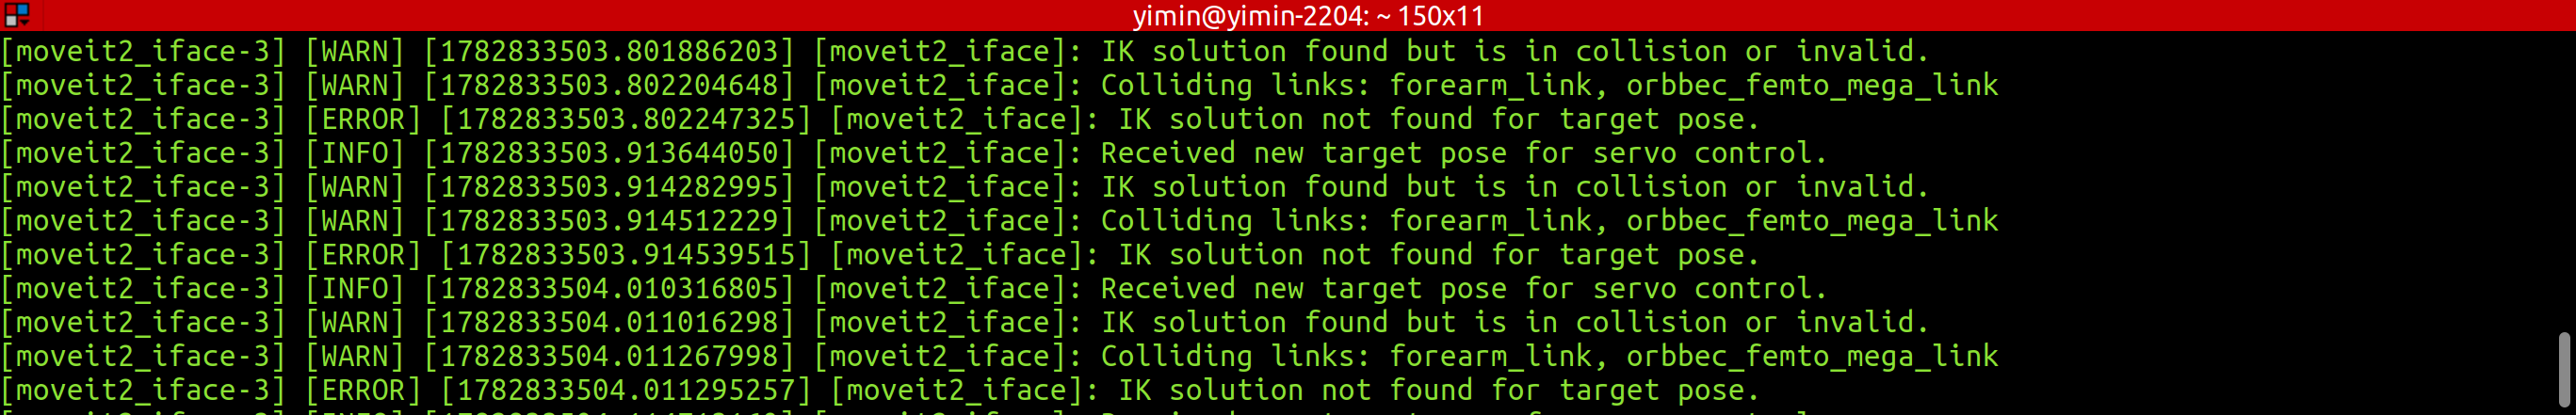
\includegraphics[width=0.95\linewidth]{F3.png}
  \caption{Failure mode F3: Kinematic infeasibility. Target pose is
    received, but the motion planner fails to find a collision-free trajectory or certain joints exceed their limits.}
  \label{fig:failure-mode-F3}
\end{figure}

\subsubsection{F4 (Orientation error)}
The pick-and-place sequence completes without a drop, but the object is placed at an inverted orientation (\cref{fig:failure-mode-F4-1} and \cref{fig:failure-mode-F4-2}). Detected by visual inspection at the placement zone.

The angle grinder is strongly asymmetric along its principal axis. A grasp that closes the Robotiq 2F-140 perpendicular to the principal axis may seat the object with its head pointing in either direction relative to the approach, producing an inverted placement.

In practice, an inverted placement does not always cause a complete pick-and-place failure: the gripper may still transport the object successfully, with the error manifesting only at placement, where the object lands in the wrong orientation for the CT scanner. F4 is therefore a downstream task failure rather than a mechanical failure, and its impact on the success metric depends on how strictly placement orientation is enforced in the trial protocol.

By introducing a new grasp axis alignment constraint, vMF-Contact assigns equal confidence to contact normals on opposite sides of the object's principal axis, which could expand the candidate set at critical positions to address F3. This would come with inverted placement as a trade-off. It is defined as future work in \cref{sec:future-work} and implemented in Appendix \cref{sec:appendix-filter-design}.


% Without an alignment constraint, the selected candidate may produce correct or inverted placement depending on which surface the top-ranked contact falls on, with no algorithm-level signal that the orientation is inconsistent. With the new grasp axis alignment constraint, this inconsistency can be detected and tolerated. This new constraintis defined as future work in \cref{sec:future-work}.

\begin{figure}[htbp]
  \centering
  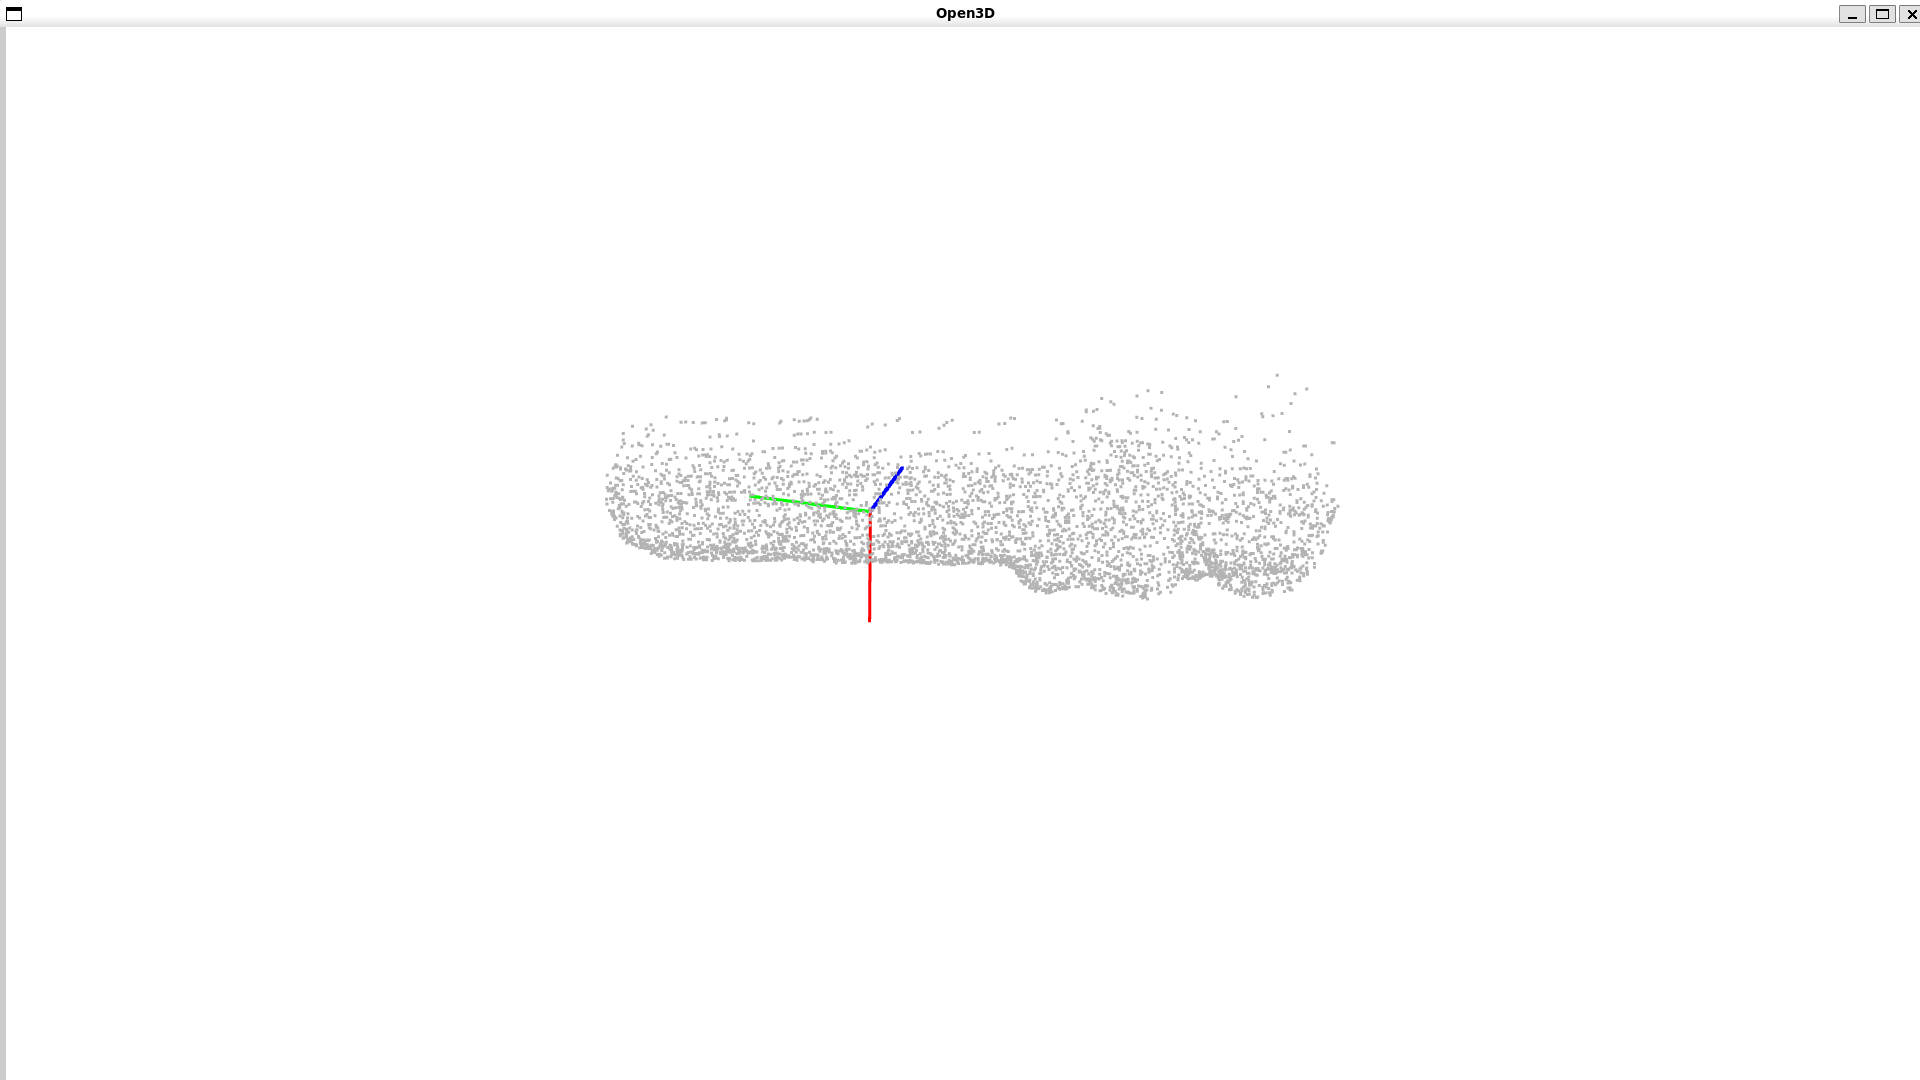
\includegraphics[width=0.6\linewidth]{F4-grasp-opp.jpg}
  \caption{Failure mode F4 in visualization. Object grasped at incorrect orientation.}
  \label{fig:failure-mode-F4-1}
\end{figure}

\begin{figure}[htbp]
  \centering
  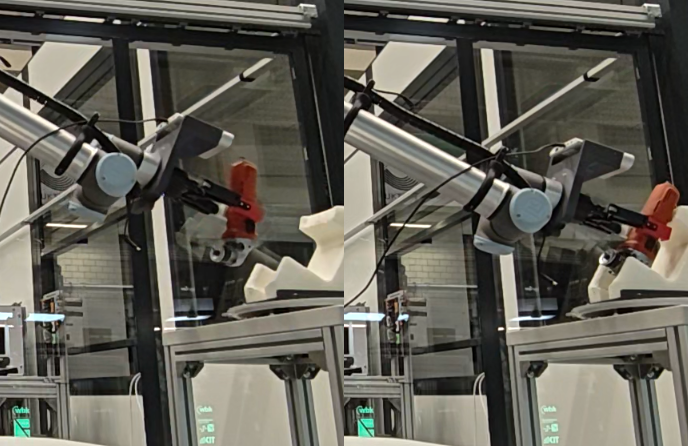
\includegraphics[width=0.6\linewidth]{F4-grasp-scene.png}
  \caption{Failure mode F4 in real scene. Object placed at incorrect orientation.}
  \label{fig:failure-mode-F4-2}
\end{figure}

\subsection{Failure Distribution by Condition}
\label{sec:failure-distribution-by-condition}

Table~\ref{tab:failure-modes} reports the failure mode distribution per condition.

\begin{table}[htbp]
  \centering
  \caption{Failure mode counts per condition (144 trials each).}
  \label{tab:failure-modes}
  \begin{tabular}{llllll}
    \toprule
    Condition & F1 (grip) & F2 (no pose) & F3 (kinematic) &
      F4 (orient.) & Success \\
    \midrule
    Baseline~1 & 103 & 0 & 11 & 10 & 20 \\
    Baseline~2 & 71  & 1 & 14 &  0 & 58 \\
    Final      &   1 & 7 & 25 &  0 & 111 \\
    \bottomrule
  \end{tabular}
\end{table}

\textbf{Baseline~1 (13.9\,\%).} F1 dominates with 103 failures (71.5\,\%): unconstrained candidate selection places grasps at object extremities remote from the centroid, producing insufficient grip force during transport. F2 does not occur (0\,\%), because no filter is active. F3 accounts for 11 failures (7.6\,\%), concentrated at orientations that require joint configurations near the UR10e workspace boundary. F4 accounts for 10 failures (6.9\,\%): without an axis alignment constraint, off-axis candidates generate placement orientation errors at delivery.

\textbf{Baseline~2 (40.3\,\%).} F1 falls from 103 to 71 (49.3\,\% of trials): centroid distance constraints concentrate candidate selection in the stable handle region, eliminating the majority of extremity grasps. Residual F1 occurs where the flat fingertip contacts the cylindrical handle surface at a marginal line-contact point insufficient to sustain grip during transport. F2 appears at 1 trial (0.7\,\%), where point cloud degradation at the handle region causes all candidates to be rejected after centroid filtering. F3 increases marginally from 11 to 14 (9.7\,\%): constraint-selected candidates at certain orientations require slightly harder joint configurations than the unconstrained top-ranked candidate, expanding the planning failure set. F4 is eliminated (0\,\%): the axis projection constraint rejects candidates whose gripper axis does not align with the object's principal axis.

\textbf{Final (77.1\,\%).} F1 falls to 1 (0.7\,\%): the custom silicone fingertip eliminates nearly all residual grip failures. F2 increases from 1 to 7 (4.9\,\%): the increment reflects inter-session point cloud variability. Final condition trials were conducted in a separate experimental session in which minor object placement offsets caused transient reductions in handle-region candidate density. No algorithmic change causes this increase. F3 increases from 14 to 25 (17.4\,\%): driven by O3 ($12\to15$) and O7 ($1\to9$). The orientation-specific F3 pattern is examined in \cref{sec:failure-distribution-by-orientation}. F4 remains 0 (0\,\%): orientation compliance is maintained at Baseline~2 level; the fingertip modification does not interact with the axis alignment constraint.

\subsection{Failure Distribution by Orientation}
\label{sec:failure-distribution-by-orientation}

\begin{table}[htbp]
  \centering
  \caption{Baseline~1 orientation cluster classification (O1--O8).}
  \label{tab:baseline1-orientation-clusters}
  \begin{tabular}{lllll}
    \toprule
    Orientation & F1 & F2 & F3 & F4 \\
    \midrule
    O1 & 10 & 0 &  0 & 2 \\
    O2 & 14 & 0 &  0 & 2 \\
    O3 & 18 & 0 &  0 & 0 \\
    O4 & 14 & 0 &  0 & 0 \\
    O5 & 15 & 0 &  0 & 2 \\
    O6 & 13 & 0 &  0 & 1 \\
    O7 &  5 & 0 & 11 & 0 \\
    O8 & 14 & 0 &  0 & 3 \\
    \bottomrule
  \end{tabular}
\end{table}

\begin{table}[htbp]
  \centering
  \caption{Baseline~2 orientation cluster classification (O1--O8).}
  \label{tab:baseline2-orientation-clusters}
  \begin{tabular}{lllll}
    \toprule
    Orientation & F1 & F2 & F3 & F4 \\
    \midrule
    O1 &  9 & 0 &  0 & 0 \\
    O2 & 16 & 0 &  0 & 0 \\
    O3 &  5 & 1 & 12 & 0 \\
    O4 &  2 & 0 &  0 & 0 \\
    O5 & 10 & 0 &  1 & 0 \\
    O6 & 11 & 0 &  0 & 0 \\
    O7 & 13 & 0 &  1 & 0 \\
    O8 &  5 & 0 &  0 & 0 \\
    \bottomrule
  \end{tabular}
\end{table}

\begin{table}[htbp]
  \centering
  \caption{Final orientation cluster classification (O1--O8).}
  \label{tab:final-orientation-clusters}
  \begin{tabular}{lllll}
    \toprule
    Orientation & F1 & F2 & F3 & F4 \\
    \midrule
    O1 & 1 & 0 &  0 & 0 \\
    O2 & 0 & 0 &  0 & 0 \\
    O3 & 0 & 3 & 15 & 0 \\
    O4 & 0 & 2 &  1 & 0 \\
    O5 & 0 & 1 &  0 & 0 \\
    O6 & 0 & 0 &  0 & 0 \\
    O7 & 0 & 0 &  9 & 0 \\
    O8 & 0 & 1 &  0 & 0 \\
    \bottomrule
  \end{tabular}
\end{table}

The 8-orientation matrix reveals structured failure patterns. Three clusters emerge from per-orientation success rate analysis in the 3 conditions.

\textbf{Epistemic uncertainty and low-confidence orientations lead to F1.} In Baseline~2 (\cref{tab:baseline2-orientation-clusters}), orientations O1, O2, O5, O6, and O7 produce elevated F1 rates (9--16 failures per orientation out of 18 trials). These orientations yield few surviving candidates after centroid filtering(typically one to two candidates) compared to five to ten at well-represented orientations. The sparse pool is consistent with high epistemic uncertainty. The vMF-Contact model has limited training coverage of these viewpoints, producing a low-density distribution that generates few high-confidence candidates within the centroid zone. The system selects from a small, low-confidence pool, increasing the probability of selecting a candidate at a marginal contact position where the flat fingertip provides insufficient grip.

\textbf{F2 elevates and F1 almost eliminates in the Final condition.} In the Final condition, F2 failures occur at a small number of orientation cells (O3\,=\,3, O4\,=\,2, O5\,=\,1, O8\,=\,1). This may be because the hardware was repositioned between sessions, causing minor variations in object placement and point cloud coverage. The F2 failures are concentrated at orientations where the handle region is partially occluded or where sensor noise degrades point cloud coverage, reducing the number of candidates that survive the centroid distance filter. In all observed F2 cases, a minor object repositioning resolved the failure in a subsequent attempt. F2 failures are recorded as failures in the trial protocol, with no repositioning permitted between delivery and execution. In a production deployment, the environment in which the object is placed should avoid scenes with complex lighting conditions, and a reposition of the object would recover the majority of these cases at negligible operational cost.

The custom silicone fingertip substantially resolves the F1 failures in the Final condition. The single residual F1 at O1 remains the only orientation-specific F1.

\textbf{F3 dominates failure at critical orientations O3 and O7 in the Final condition.} O3 and O7 account for 24 of the 25 F3 failures in the Final condition and constitute the primary F3 cluster (\cref{tab:baseline1-orientation-clusters}--\cref{tab:final-orientation-clusters}).

The F3 pattern at O3 is mostly caused by the newly introduced constaints rather than an intrinsic property of the kinematic envelope. In Baseline~1, unconstrained candidate selection produces kinematically accessible poses at O3. All 18 trials proceed to motion planning, but all fail through grip force insufficiency (F1\,=\,18, F3\,=\,0). Once centroid distance constraints restrict candidate selection in Baseline~2, the feasible candidate set at O3 is confined to approach angles near the UR10e workspace boundary, producing F3\,=\,12. The pattern intensifies in the Final condition (F3\,=\,15, F2\,=\,3). O3 achieves zero successes across all three conditions.

At O7, F3 rates vary across conditions (Baseline~1: 11, Baseline~2: 1, Final: 9). The anomalously low Baseline~2 rate likely reflects session-level sampling variance: centroid-constrained candidate selection at O7 happened to favour kinematically accessible poses in the Baseline~2 session, while both the Baseline~1 and Final sessions encountered workspace boundary more frequently due to minor inter-session differences in object placement.

Both orientations are included in the full-matrix success rate denominator, as they represent real failure conditions in the deployment. If we exclude O3 and O7 from the final result, the success rate over the six kinematically productive orientations (O1, O2, O4, O5, O6, O8) is \textbf{94.4\,\%}. It is actually a satisfactory considering the complexity of the task case.

Therefore, one practical solution to this failure mode could be to avoid the critical orientations O3 and O7 in deployment, either by instructing the AGV to deliver the object in a different orientation or by rotating the object in situ before grasping. This is a simple operational mitigation that does not require any algorithmic change.

Another practical solution to this failure mode would be to substitute the object axis alignment constraint at these critical orientations (O3, O7 and possibly O5) with a new reachability filter. It only limits candidates to those whose gripper axis is limited to the frontal direction of the robot station, rather than enforcing a strict orientation or alignment to the object principle axis. This would expand the candidate set at O3 and O7, allowing the planner to select kinematically feasible poses. But it comes with inverted placement at these orientations as a trade-off. It is defined as future work in \cref{sec:future-work}.

\subsection{Failure Distribution by Position}
\label{sec:failure-distribution-by-position}

\begin{table}[htbp]
  \centering
  \caption{Baseline~1 position cluster classification (P1--P6).}
  \label{tab:baseline1-position-clusters}
  \begin{tabular}{lllll}
    \toprule
    Position & F1 & F2 & F3 & F4 \\
    \midrule
    P1 & 16 & 0 & 2 & 3 \\
    P2 & 17 & 0 & 3 & 3 \\
    P3 & 16 & 0 & 3 & 1 \\
    P4 & 15 & 0 & 3 & 0 \\
    P5 & 20 & 0 & 0 & 2 \\
    P6 & 19 & 0 & 0 & 1 \\
    \bottomrule
  \end{tabular}
\end{table}

\begin{table}[htbp]
  \centering
  \caption{Baseline~2 position cluster classification (P1--P6).}
  \label{tab:baseline2-position-clusters}
  \begin{tabular}{lllll}
    \toprule
    Position & F1 & F2 & F3 & F4 \\
    \midrule
    P1 & 11 & 0 & 2 & 0 \\
    P2 & 14 & 1 & 1 & 0 \\
    P3 & 12 & 0 & 3 & 0 \\
    P4 & 11 & 0 & 1 & 0 \\
    P5 & 13 & 0 & 3 & 0 \\
    P6 & 10 & 0 & 4 & 0 \\
    \bottomrule
  \end{tabular}
\end{table}

\begin{table}[htbp]
  \centering
  \caption{Final position cluster classification (P1--P6).}
  \label{tab:final-position-clusters}
  \begin{tabular}{lllll}
    \toprule
    Position & F1 & F2 & F3 & F4 \\
    \midrule
    P1 & 0 & 0 & 5 & 0 \\
    P2 & 0 & 3 & 0 & 0 \\
    P3 & 0 & 0 & 5 & 0 \\
    P4 & 0 & 0 & 4 & 0 \\
    P5 & 1 & 1 & 6 & 0 \\
    P6 & 0 & 3 & 5 & 0 \\
    \bottomrule
  \end{tabular}
\end{table}

Position effects are secondary to orientation effects. Success rate variation across the six positions within any given orientation is small relative to the inter-orientation variation.

\textbf{F1 and F3 show no clear pattern across positions.} In Baseline~1 (\cref{tab:baseline1-position-clusters}), F1 is the dominant failure mode and is distributed across all six positions (P1--P6) with no clear pattern. In Baseline~2 (\cref{tab:baseline2-position-clusters}), F1 is reduced but remains evenly distributed across positions. In the Final condition, F1 is nearly eliminated and does not show any position-specific clustering. F3 is also mostly evenly distributed across positions. The position effect on F3 is likely a secondary consequence of the orientation effect. Certain orientations produce kinematically challenging poses that are more likely to occur at specific positions due to the robot's reachability envelope.

\textbf{F2 is concentrated at P2 and P6.} P2 and P6 have higher F2 incidence compared to other positions (\cref{tab:final-position-clusters}). P2 and P6 are positions where the object is placed closer to the robot. This may lead to partial occlusion, reducing the number of contact candidates that survive the centroid distance filter. A minor object repositioning would resolve the failure in a subsequent attempt as described in \cref{sec:failure-distribution-by-orientation}.

\section{Summary}
\label{sec:results-summary}

\subsection{Interpreting the Three-Condition Results}

The three-condition design gives us two measurements of how things are affected, and it is clear what is causing these effects.

The change from Baseline~1 to Baseline~2, which is from 13.9\,\% to 40.3\,\%, shows us how much the software is contributing to the results when the hardware is not changing. The change from Baseline~2 to the Final result, which is from 40.3\,\% to 77.1\,\%, shows us how much the custom fingertip is contributing to the results when the algorithm is not changing. 

We should pay attention to the Baseline~1 result. When the success rate is 13.9\,\% out of 144 tries, it means the algorithm without any changes only works in fewer than one out of six attempts. If we compare this to the vMF-Contact algorithm, which gets 72.7\,\% right in a controlled test~\cite{shi2025}, we can see that the basic algorithm is not good enough to use without some changes in this situation. The two changes we made to the algorithm, which are based on the shape of the objects, are necessary for this to work and not just a way to make up for things in the environment.

The Baseline~2 result, which is 40.3\,\%, shows that even when we limit the grasp zone to a certain area which tends to have a higher grasp success rate, it still fails half the time because the gripper does not have enough grasp force when it lifts and moves the objects. The custom fingertip is fixing a problem with the hardware that we cannot fix by changing the algorithm. When we use both the algorithm and the custom fingertip together, we get a better result, which is 77.1\,\%.

Final results showed that our system performed well in the harder test case compared to the test case used in the~\cite{shi2025} paper. We used less force to grasp the objects compared to the test case (125\,N vs 235\,N) and the objects were much heavier (approximately 2\,kg vs 1\,kg) and we were testing a complete task of picking, transport and grasping of objects. Therefore, the test case was much hard than the test cases used in the paper, but the system performed well. This shows that the modifications made to the system worked well.

This does not mean that our changed system is better than the algorithm in all situations. It just shows that the changes we made are working for this certain longitudinal and asymmetric geometry.

\subsection{Failure Mode Analysis: Causes and Implications}
\label{sec:failure-mode-analysis-discussion}

Understanding the causes of residual failures in the Final condition is more useful for guiding future work than the top-line success rate.

\textbf{Epistemic uncertainty and the low-confidence orientation cluster.} The orientation-dependent F1 cluster identified in \cref{sec:failure-distribution-by-orientation} reflects the epistemic uncertainty property of the vMF-Contact model discussed in \cref{sec:industrial-deployment-gap}. At orientations underrepresented in the training distribution, the model produces low-density vMF distribution. Fewer grasp candidates fall within the centroid zone. 

% Even though the system selects the highest-ranked surviving candidate, this candidate is still likely to fall at the boundary of the mechanically stable grip zone, where the flat fingertip provides insufficient friction to hold a 2\,kg object through a full transport trajectory.

% The failure sequence --- high epistemic uncertainty $\rightarrow$ sparse centroid-filtered candidates $\rightarrow$ boundary contact selection $\rightarrow$ F1 --- validates the theoretical motivation for probabilistic uncertainty modelling introduced in \cref{sec:uncertainty-aware-grasping}.

It also identifies the appropriate intervention. (1) \textbf{A custom designed silicone fingertip}, which is introduced in \cref{sec:custom-fingertip-design} and implemented in the Final condition shows substantial improvement in grasp performance. (2) \textbf{Orientation pre-screening at delivery time.} By placing the object on the AGV toward orientations and in positions with known high success rate, it is less likely that we will come with low coverage problems of the point cloud. (3) \textbf{Additional viewpoints.} Another solution to occlusion or low coverage point cloud is to fuse several point cloud from multiple viewpoints to a more complete one. This would inevitably come with longer processing time as a trade-off. 

\textbf{Positional sensitivity.} F2 failures usually occur at certain positions and certain lighting environment. In all observed cases, a minor repositioning of the object resolved the failure in a subsequent attempt. It is suggested not to put the object too close to the robot, or under a straight downlight, where the reflexion from the object surface may cause noise in the point cloud.

\textbf{Kinematic infeasibility.} F3 failures at specific orientations reflect the UR10e workspace boundary, not algorithm or hardware behaviour. The appropriate solution is a pre-execution reachability check that aligns the grip axis with the object principal axis (in both directions) before final selection. Integrating and validating this filter on the current trial matrix is the most direct path to reducing F3 failures and improving the full-matrix success rate beyond 77.1\,\%. It is defined as future work in \cref{sec:future-work} and analyzed in Appendix \cref{sec:appendix-results}.

\section{Deployment Recommendations}
\label{sec:deployment-recommendations}

The results and limitations define a specific operating envelope. The current system is suited to some industrial contexts and not others, and the boundary between them follows directly from the failure mode analysis.

\textbf{Suitable contexts.} The system is suitable for a circular factory return stream of \textbf{single objects} of \textbf{known type} that are delivered by an AGV to a variable position and orientation. The stream has a moderate throughput that can be processed within a 3--5\,s latency period of the down-stream pipeline. The system should be deployed in work environment with \textbf{soft lighting condition}. Operationally the system can run with a 77.1\% first-attempt success rate with a retry path or manual intervention. In the current cell F1 failures can be visually detected. F2 and F3 failures are reported by the inference and planning nodes. This \textbf{detection and feedback machanism} is a prerequisite for any automated retry and deployments without it cannot safely run a retry loop.


% The system is well-matched to circular factory return streams: single objects of a known class delivered by AGV at variable position and orientation, moderate throughput compatible with a 3--5\,second pipeline latency, and an operational tolerance for a 77.1\,\% first-attempt success rate with a retry path for failed attempts. In the current cell, F1 failures (object dropped mid-trajectory) are detected via visual inspection. F2 and F3 failures are reported by the inference and planning nodes respectively. This detection infrastructure is a prerequisite for any retry loop. Deployments without it cannot safely implement automated retry. The broader class of circular manufacturing scenarios shares the cell's operating properties and fits the system's envelope for the same reasons.

\textbf{Unsuitable contexts.} \textbf{High-takt automated assembly lines} are outside the current operating envelope: the inference-and-planning latency is incompatible with short cycle times, and a single F3 or F1 failure interrupts the line. \textbf{Multi-object cluttered scenes} require an instance segmentation module before the centroid constraints become applicable. \textbf{Safety-critical applications} requiring reliability above 95\,\% would need the F3 reachability filter, epistemic uncertainty mitigation, and additional validation before deployment. \textbf{Novel object geometries} require re-parameterisation of the centroid constraints and fingertip contact validation because the current parameters are specific to the angle grinder and should not be applied to other object classes without verification.

Each unsuitability is addressable through specific future work. The work from my thesis could be a validated starting point for industrial learning-based grasping. 


% ============================================================
\chapter{Conclusion}
\label{chap:conclusion}
% ============================================================

\section{Summary}
\label{sec:conclusion-summary}
A factorial evaluation across 432 trials under three conditions, (1) unconstrained baseline~1, (2) constrained algorithm baseline~2, and (3) constrained algorithm with custom fingertip final, isolates the contribution of each adaptation. 

Baseline~1 achieves 13.9\,\% success. Baseline~2 raises this to 40.3\,\%. Final condition raises it further to 77.1\,\%. The 77.1\,\% result exceeds the published vMF-Contact benchmark of 72.7\,\% despite three compounding deployment disadvantages: 47\,\% lower grip force, twice the object weight, and a stricter full pick-transport-place success criterion. Failure mode analysis identifies constraint-induced kinematic infeasibility as the dominant residual failure mechanism.

% This thesis asked: to what extent can the pick-and-place with unconstrained vMF-Contact algorithm work in a real production scenario? What other constraints can be applied to improve the grasping success rate of an angle grinder compared to unconstrained vMF-Contact inference?

% The answer is unambiguous. Unconstrained vMF-Contact inference achieves a success rate of 13.9\,\% on the $3 \times 8 \times 6$ trial matrix. Centroid-based constraints raise this to 40.3\,\%. The addition of a custom curved silicone fingertip raises it further to 77.1\,\%. The improvement from constraints alone (approximately 26.4 percentage points) demonstrates that the algorithmic adaptation is both necessary and effective. The further improvement from the fingertip (approximately 36.8 percentage points) demonstrates that hardware-object compatibility is an independent, load-bearing factor that no algorithm modification can substitute for.

Four contributions realise these results.

\textbf{Contribution~A} introduces two centroid-based constraints into the vMF-Contact inference pipeline. An annular grip zone defined relative to the object's geometric centroid proxy, and a gripper-axis alignment constraint with the object's principal axis. These aim to address grip force insufficiency and orientation error, which are the two dominant failure modes of unconstrained inference on this task. 

\textbf{Contribution~B} is a custom fingertip for the Robotiq 2F-140, incorporating a curved contact surface matched to the angle grinder handle and a silicone friction layer, which addresses the grip force with a broader contact area and additional friction force.

\textbf{Contribution~C} is the ROS2 and Docker integration pipeline that enables reproducible deployment of the full system on the UR10e cell.

\textbf{Contribution~D} is the structured deployment evaluation, which isolates the effects of algorithmic and hardware adaptation, stratifies failure modes by orientation and position, and identifies residual failure clusters for future work. The evaluation gives us a better insight of different failure modes and their causes, as well as potential solution to them.

\section{Research Gaps Addressed}
\label{sec:research-gaps-addressed}

\textbf{Gap A --- Missing geometric priors.} Prior learning-based grasping methods, including vMF-Contact, encode local contact geometry but not object-level spatial relationships. The centroid-based constraints introduced in Contribution~A directly address this omission. The Baseline~1 to Baseline~2 result provides quantitative evidence that these priors are necessary for this task class: without them, the algorithm fails on nearly every trial.

\textbf{Gap B --- Absence of systematic deployment evaluation.} Prior work provides benchmark comparisons but not structured deployment studies with failure mode analysis, real hardware-object constraints, and a full pick-transport-place success criterion. The 432-trial evaluation across three conditions, eight orientations, and six positions fills this gap for the specific deployment studied here. The failure mode analysis demonstrates what this style of evaluation reveals that isolated benchmarks do not: the specific conditions under which a validated method succeeds and fails in a real industrial cell.

\section{Limitations}
\label{sec:limitations}

\textbf{Object-specificity of centroid parameters.} The centroid distance thresholds ($d_{\max}$ = 0.025\,m, $d_{\min}$ = 0.01\,m) and $th_{axis\_proj}$ are calibrated to the angle grinder's geometry. Extending the system to a second class requires repeating the parameter validation procedure. Whether a unified parameter set generalises across a family of elongated asymmetric objects remains an open question.

\textbf{Single-object scene requirement.} The centroid proxy is computed from the full filtered point cloud without instance segmentation. In a multi-object scene, the computed centroid averages across all objects present, making the spatial filter inevitably unsuitable. The system therefore requires single-object placement in the delivery zone. This is a constraint of the centroid approach, not of vMF-Contact itself. 

\textbf{Residual F3 failures.} The F3 failure cluster at specific orientations is unaddressed in the current experimental system. These failures are primarily a function of the UR10e workspace geometry and the induced by the constraints. F3 rates rise across conditions as constraints progressively restrict candidate selection toward workspace-boundary poses. The pre-emptive reachability filter is the appropriate solution. It will be introduced in Appendix \cref{sec:appendix-motivation}.

\textbf{Model coverage at specific orientations.} The epistemic uncertainty cluster identifies orientations at which the vMF-Contact model has limited training coverage of the angle grinder. This cannot be resolved through the constraint modifications alone. Additional viewpoints would address the potential F2 failures in this cluster.

\textbf{Gripper selection trade-off.} The Robotiq 2F-140 was chosen for geometric compatibility with the angle grinder handle at the cost of a 47\,\% reduction in grip force relative to the 2F-85 (125\,N versus 235\,N). The custom fingertip partially compensates for this, but does not restore grip force to 2F-85 levels. A gripper offering both wide jaw opening and higher force would likely improve performance further while preserving geometric compatibility.

\section{Future Work}
\label{sec:future-work}

Four directions follow directly from the limitations identified in \cref{sec:limitations}.

\textbf{Kinematic reachability filter.} F3 failures at specific orientations are the most directly addressable residual failure mode. A prototype reachability filter that evaluates kinematic feasibility before candidate selection is implemented in Appendix \cref{sec:appendix-filter-design}. Integrating and validating this filter on the current trial matrix is the most immediate path to improving the full-matrix success rate beyond 77.1\,\%, without changes to the algorithm or hardware.

\textbf{Instance segmentation for multi-object scenes.} The current system requires single-object placement because the centroid proxy is computed from the full point cloud. Adding an instance segmentation module, e.g. a PointNet++~\cite{qi2017pointnet2} segmentation head or a dedicated 3D network would restore the ability to handle cluttered multi-object scenes while preserving the centroid constraint logic. 

\textbf{Parameter generalisation.} The centroid distance and axis projection thresholds are calibrated to the angle grinder's geometry. Validating whether a common parameter set applies across a family of elongated asymmetric objects, or deriving the thresholds analytically from measurable object properties (handle length, centroid offset, gripper jaw width), would reduce the per-class calibration overhead and extend the system's practical range.

\textbf{Mobile robot station.} The current robot system still requires external power supply and Ethernet connection, which makes it hard to move as a unit between different cells in the circular factory. Designing a more mobile platform for it would improve its applicability in the future.

% \section{Closing}
% \label{sec:closing}

% Learning-based grasping methods achieve strong benchmark performance. The central finding of this thesis is an answer to why industrial deployment consistently falls short: algorithms encode no object-level geometric priors, hardware-object compatibility is absent from evaluation protocols, and benchmark success criteria measure a narrow proxy for the system-level outcome that deployment requires.

% The adaptations introduced here, including centroid-based constraints and a purpose-designed fingertip, are not patches on a broken method. They are the minimum necessary engineering to connect a laboratory-validated algorithm to a specific deployment context. That connection required understanding what the algorithm could not do, why the hardware was insufficient, and how to measure both in a way that separates their contributions. The result --- 77.1\,\% success on a task the base algorithm failed at 13.9\,\% --- is evidence that the gap between benchmark and deployment is structured and closeable. Closing it systematically, across object classes and deployment contexts, is the work that remains.


% ============================================================
% BACK MATTER (Roman page numbers resume)
% ============================================================
\backmatter
\listoffigures
\newpage
\listoftables
\tocloftpagestyle{scrheadings}

% Bibliography
% Note: \bibliographystyle is set to 'wbk' by wbk.cls — do NOT call
% \bibliographystyle here or it will override the class setting.
% The wbk style uses author-year (natbib) formatting.
% If you need IEEE numbered citations, switch to \documentclass[...]{report}
% and restore \usepackage{cite} + \bibliographystyle{IEEEtran}.
\cleardoublepage
\phantomsection \addcontentsline{toc}{chapter}{\bibname}
% Uncomment the next line if BibTeX reports errors about '_' in URLs/DOIs:
% \newcommand_[1]{\text{\_#1}}
\bibliography{references}

\clearpage{\pagestyle{scrheadings}\cleardoublepage}

% Appendix — figure/table counters restart as A.1, A.2 ...
\renewcommand{\thefigure}{A.\arabic{figure}}
\renewcommand{\thetable}{A.\arabic{table}}
\newcommand_[1]{\ensuremath{\sb{\scriptscriptstyle #1}}} \setcounter{figure}{0}
\chapter{Appendix}
\label{chap:appendix}
\thispagestyle{empty}
\quad \addtocounter{page}{-1}
% \newpage

% \chapter{Kinematic Reachability Filter}
% \label{chap:appendix-reachability}

\section{Motivation}
\label{sec:appendix-motivation}

In the Final condition (\cref{sec:failure-mode-analysis}), kinematic infeasibility (F3) is the dominant residual failure mode: 25 of 144 trials (17.4\,\%) end in motion-planner failure. Two orientations account for 96\,\% of these failures: O3 (15 of 18 trials) and O7 (9 of 18 trials). O3 achieves zero successes across all three experimental conditions.

% The F3 pattern is constraint-induced rather than intrinsic to the robot's workspace. In Baseline~1, unconstrained vMF-Contact inference selects kinematically accessible candidates at O3 and O7 — all 18 O3 trials reach the motion planner, but all fail through grip force insufficiency (F1\,=\,18, F3\,=\,0). The centroid distance constraints introduced in Contribution~A confine candidate selection to the handle region, but handle-region candidates at O3 and O7 systematically require approach angles near the UR10e workspace boundary. The motion planner then fails to find collision-free joint trajectories, producing F3 failures.

Two operational mitigations were identified in \cref{sec:failure-mode-analysis-discussion}: restricting AGV delivery to orientations outside the F3 cluster, or adding a pre-execution reachability check that filters candidates with approach geometries unlikely to be kinematically feasible before the motion planner is invoked. This appendix describes the second approach, implemented and evaluated after the main controlled experiment reported in \cref{chap:experimental-setup-and-results}.

\section{Filter Design}
\label{sec:appendix-filter-design}
\begin{figure}
  \centering
  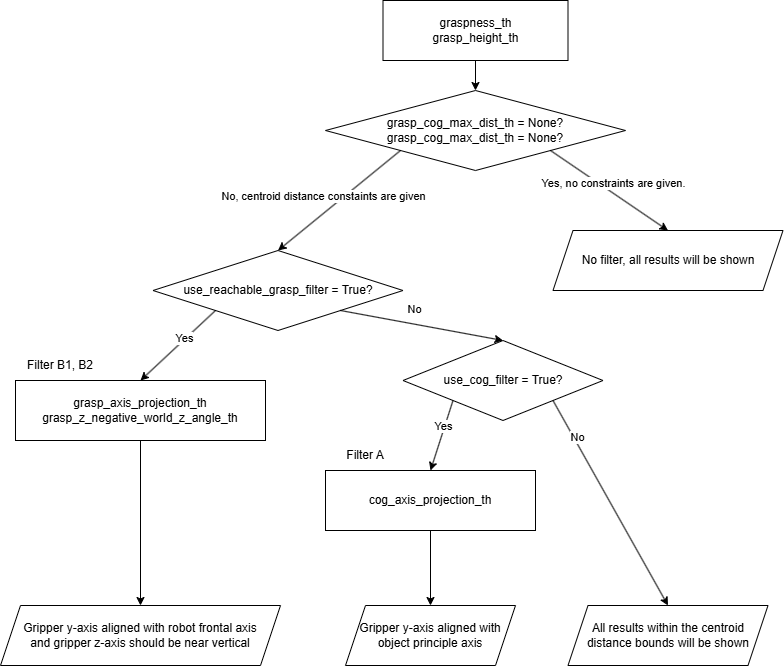
\includegraphics[width=0.95\linewidth]{filter-cascade-diagram.png}
  \caption{This figure shows the filter cascade architecture.}
  \label{fig:filter-cascade}
\end{figure}

The reachability filter extends the existing constraints set of \cref{sec:vmf-contact-inference} with two additional directional constraints on the grasp approach geometry. Both checks are geometric heuristics — lightweight vector operations computed from the candidate pose — that pre-discard approach directions associated with workspace-boundary configurations without invoking the IK solver or motion planner. A detailed filter cascade diagram is shown in \cref{fig:filter-cascade}.

\paragraph{Filter B1 — Frontal projection constraint.}

\begin{figure}
  \centering
  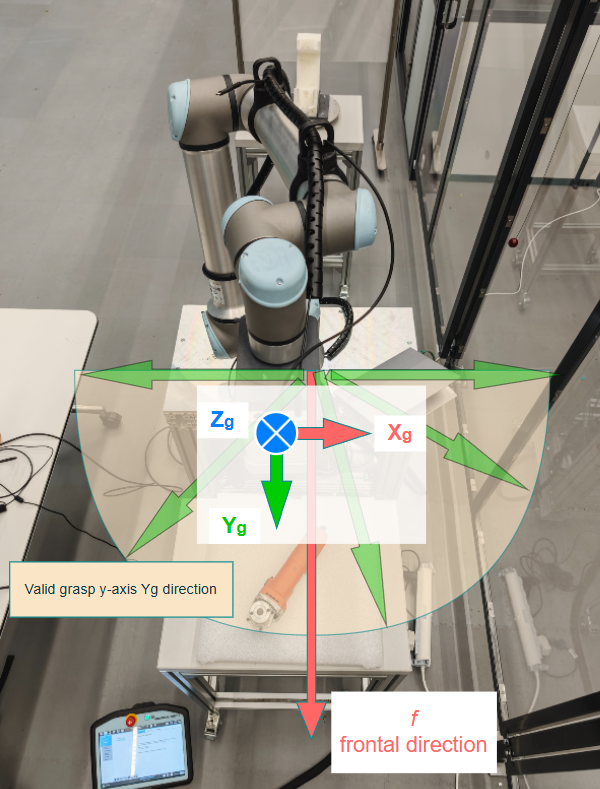
\includegraphics[width=0.95\linewidth]{frontal-overview-1.png}
  \caption{This figure shows the actual spatial representation of the frontal projection constraint. The gripper y-axis \param{y\ensuremath{\sb{g}}} should be facing the robot's frontal direction $\mathbf{f}$.}
  \label{fig:frontal-overview}
\end{figure}

\begin{figure}
  \centering
  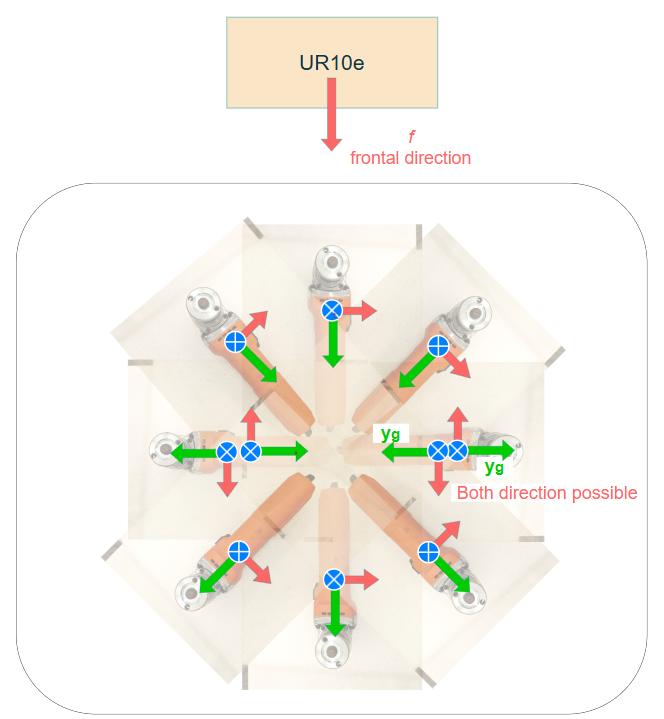
\includegraphics[width=0.95\linewidth]{frontal-orient.png}
  \caption{A representation of the possible object orientations and the gripper \param{y\ensuremath{\sb{g}}} axis after applying the frontal projection constraint.}
  \label{fig:frontal-orient-grasp}
\end{figure}

The UR10e's nominal frontal direction is defined as $\mathbf{f} = [-1,\,0,\,0]^{\!\top}$ in the world frame. For each surviving candidate, the projection of the gripper closing axis \param{y\ensuremath{\sb{g}}} onto $\mathbf{f}$ is computed:
\begin{equation}
  p = \param{y\ensuremath{\sb{g}}} \cdot \mathbf{f}.
\label{eq:frontal-projection}
\end{equation}
Candidates with $p \leq $th_{frontal}$ (\param{grasp\_axis\_projection\_th}) = 0$ are discarded. The threshold of zero requires a strictly positive projection, ensuring the gripper faces into the robot's primary workspace. Grasps directed away from the robot require shoulder and elbow joints to approach their limits in order to reach the target pose and is hense rejected. As shown in \cref{fig:frontal-overview}.

A figure that represents the possible grasp poses after applying this filter is shown in \cref{fig:frontal-orient-grasp}. Note that there may be 2 possible grasp orientations at the two horizontal inital orientations, as their gripper y-axis \param{y\ensuremath{\sb{g}}} may either has a positive projection to the frontal axis $\mathbf{f}$, or not.


\paragraph{Filter B2 — Vertical approach constraint.}

\begin{figure}
  \centering
  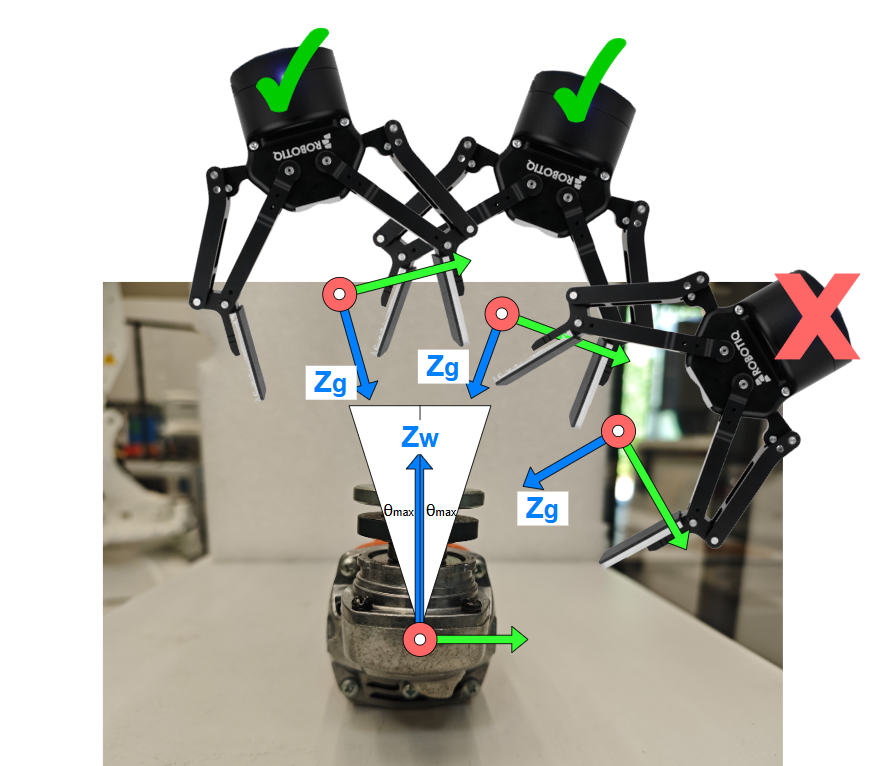
\includegraphics[width=0.95\linewidth]{vertical-grasp.png}
  \caption{This figure shows valid grasp pose after applying the filter B2-vertical approach constraint. The gripper's approach axis \param{z\ensuremath{\sb{g}}} (the z-axis of the gripper frame) is constrained to remain within $\theta_{\max}$ of the world z-axis $\param{z\ensuremath{\sb{w}}}$:}
  \label{fig:vertical-grasp}
\end{figure}

The gripper's approach axis \param{z\ensuremath{\sb{g}}} (the z-axis of the gripper frame) is constrained to remain within $\theta_{\max}$ of the world z-axis $-\param{z\ensuremath{\sb{w}}}$:
\begin{equation}
  \angle\!\left(\param{z\ensuremath{\sb{g}}}\,-\param{z\ensuremath{\sb{w}}}\right) \;\leq\; \theta_{\max}.
\label{eq:vertical-approach}
\end{equation}
The threshold $\theta_{\max}$($\param{grasp\_z\_negative\_world\_z\_angle\_th}) = 10^{\circ}$ is applied. Candidates exceeding this angle are discarded (\cref{fig:vertical-grasp}).

% A near-vertical approach minimises wrist rotation demand and keeps the end-effector in the region of the UR10e workspace where the redundancy resolver reliably produces joint-limit-safe configurations. At O3 and O7, handle-region candidates after centroid filtering tend to have tilted approach vectors because the object's handle faces directions that require non-vertical gripper entry at those orientations; the vertical constraint pre-filters these candidates before the motion planner is invoked.

A near-vertical approach minimises wrist rotation possibility and keeps the end-effector in the region of proper grasp workspace where the gripper would not approach the object from the side. This helps avoid tilted approach and eventually manual adjustment after placement because of the object face direction.

There are three level filter switches in the final filter cascade. The \param{grasp\_cog\_max\_dist\_th} and \param{grasp\_cog\_max\_dist\_th} are the first level switch. By setting value to them, grasp zone will be limited to a certain area around the geometric centroid proxy, as described in \cref{sec:centroid-distance-constraints}. Otherwise, the node will work as the base vMF-Contact algorithm and no grasp candidates will be filtered. \param{use\_reachable\_grasp\_filter} is the second level switch to this cascade, which determines whether to use the filter B1 and B2 introduced in this chapter. It is parallel to Filter A, which is introduced in \cref{sec:axis-alignment-constraint}. But nly one group of filter can take in effect. This is the function of the third level filter \param{use\_cog\_filter}. They cannot exist at the same time as the axis alignment constaints is not compatible with the front direction constraints. With Filter A, grasp poses whose gripper y-axis is aligned with object principle axis are passed down. With Filter B1, grasp poses whose gripper y-axis is aligned with robot frontal axis are passed down. And candidate set will be sorted again based on B2. Those with gripper z-axis orientation out of the threshold will be filtered.

\section{Experimental Results}
\label{sec:appendix-results}

The evaluation uses a reduced factorial matrix: 8 object orientations (O1--O8) $\times$ 1 delivery position $\times$ 3 repetitions per cell, yielding 24 trials in total. The hardware and software configuration matches the Final condition: centroid-based constraints active ($d_{\max}$\,=\,0.025\,m, $d_{\min}$\,=\,0.01\,m, $th_{axis\_proj}$\,=\,0.5), custom curved silicone fingertips, UR10e + Orbbec Femto Mega + Robotiq 2F-140. The success criterion follows \cref{sec:success-criterion} (full pick-transport-place completion without object drop) and is extended with a placement-quality sub-category, and counted as completed trials in the Success column: \textbf{PS} flags trials where the object is placed inverted relative to the intended target pose. \cref{sec:appendix-limitations} discusses the tradeoff this category reflects.

The reduced matrix isolates orientation effects at a single position. Per-orientation results are directly comparable to the Final condition per-orientation counts in \cref{tab:appendix-results} at the evaluated position, isolating the effect of the reachability filter from position-level variation.

\begin{table}[htbp]
  \centering
  \caption{Reachability filter evaluation: per-orientation failure counts and success (8\,orientations $\times$ 1\,position $\times$ 3\,trials\,=\,24\,trials total).}
  \label{tab:appendix-results}
  \begin{tabular}{lrrrrr}
    \toprule
    Orient. & F1(grip) & F2(no pose) & F3(kin.) & PS(Inverted orient.) & Success \\
    \midrule
    O1 & 0 & 0 & 0 & 2 & 3 \\
    O2 & 0 & 0 & 0 & 2 & 3 \\
    O3 & 0 & 0 & 0 & 3 & 3 \\
    O4 & 0 & 0 & 0 & 0 & 3 \\
    O5 & 0 & 0 & 0 & 3 & 3 \\
    O6 & 0 & 0 & 0 & 0 & 3 \\
    O7 & 0 & 0 & 0 & 3 & 3 \\
    O8 & 0 & 0 & 0 & 0 & 3 \\
    \midrule
    \textbf{Total} & 0 & 0 & 0 & 13 & \textbf{24 / 24} \\
    \bottomrule
  \end{tabular}
\end{table}

\cref{tab:appendix-results} summarises the overall grasping results for the new 24 trials. It delivered 100\,\% success across all orientations, with no F1, F2, or F3 failures. The residual placement defect (PS) is discussed in \cref{sec:appendix-limitations}.

\section{Summary and Limitations}
\label{sec:appendix-analysis}

\subsection{Summary}
\label{sec:appendix-f1f3}

Across all 24 trials, F1, F2, and F3 are fully eliminated (Table~\ref{tab:appendix-results}), including at O3 and O7, which achieved zero and low successes respectively across all three conditions in the main experiment (\cref{sec:failure-distribution-by-orientation}).

The Fontal projection constraint (Filter B1) filters candidates whose gripper y-axis poses to the frontal direction of the robot station, which is the direct mechanism for the F3 elimination at these two orientations. Unlike the anticipated risk that a tighter candidate set at O3 and O7 would convert F3 trials into F2 trials, no F2 failures occur anywhere in the reduced matrix: the surviving candidate sets at every orientation retained at least one candidate that satisfied both new filters.  The vertical approach constraint (Filter B2, $\theta_{\max} = 10^{\circ}$) removes tilted gripper approach direction candidates before the motion planner is invoked.

% The two filters also leave F1 unaffected, consistent with the two filters acting on approach geometry rather than on centroid-zone membership or axis alignment.

\subsection{Limitations}
\label{sec:appendix-limitations}

The two new filters are geometric heuristics, not exact kinematic feasibility checks. On the one side, a candidate that passes both filters is not guaranteed to be reachable. On the other side, a candidate that fails one filter may in some cases be reachable via an alternative IK solution. The $10^{\circ}$ threshold for the vertical approach constraint was set empirically based on observation of F3 failure poses and has not been optimised over a parameter grid. A too tight threshold would increase F2. One that is too loose provides insufficient F3 reduction. The precise operating range of the threshold is an open question for future work.

\textbf{Uninvestigated: position sensitivity.} The reachability filter was evaluated at a single position. Although it has been discussed in \cref{sec:failure-distribution-by-position} that in previous experiments the failures show no position-specific clustering, it is based on the filter A. Object Position may affect the completeness of the object in point cloud as well, if the camera always stays at the same viewpoint. Position-dependent effects are not evaluated in this set of expreiment and remain a direction for further investigation.

\textbf{Tradeoff of the reachability filter: inverted placement.} Eliminating F1--F3 does not come without cost. Of the 24 trials, 13 are placed inverted relative to the intended target pose (\textbf{PS}); only O4, O6 and O8 are entirely free of a placement defect. O3, O5, and O7 are inverted in all three trials.

This is a direct tradeoff of the frontal projection constraint (Filter B1, Eq.~\eqref{eq:frontal-projection}). Filter B1 selects candidates whose gripper y-axis projects positively onto the robot's frontal direction $\mathbf{f}$, without reference to which end of the object's principal axis the candidate sits on. At orientations where the axis-alignment filter (Filter A) leaves viable candidates on both ends of the principal axis, Filter B1 can select the end that satisfies the reachability heuristic rather than the end consistent with the fixed placement target. Because the placement stage executes a single hardcoded target pose regardless of which end of the object was grasped, a candidate selected from the "wrong" end arrives inverted at the delivery position. Since the reversed placement does not have a corresponding placement target pose, in some cases the object must be manually reoriented after placement to be usable.

This tradeoff is acceptable for the current implementation. No trial drops the object ($\text{F1}$), fails to reach a valid pose ($\text{F2}$), or exceeds the robot's kinematic limits ($\text{F3}$). The inverted orientation is immediately visible upon placement, and is acceptable for subsequent CT inspections, as long as it lands on the holder. Exchanging a hard failure (F3, requiring a full retry cycle) for an immediately observable placement defect is a net improvement in a supervised deployment setting, even though it introduces a correction burden that Filters B1 and B2 alone do not remove. A flexible placement stage that recognizes the orientation and grasp point of the object being grasped and gives out a corresponding placement pose, rather than relying on a single hardcoded target pose, is left for future work.

\end{document}
